% $Id: BASENAME-main.tex 29035 2021-05-20 04:30:23Z beringer $
% Main file for PDG review ml
%
% This file is included by the top-level file ml.tex and is where the
% text of your review should be included. If desired, you may split your review into multiple
% files that are included from this file using \input.
%
% Do NOT modify the top-level file ml.tex - it is generated from
% the PDG database and all manual changes WILL BE LOST!

%Probability: \url{https://pdg.lbl.gov/2020/reviews/rpp2020-rev-probability.pdf}

%Statistics: \url{https://pdg.lbl.gov/2020/reviews/rpp2020-rev-statistics.pdf}

%Deadline  for providing a draft of your review for refereeing is \textbf{August 27, 2021.}

%\begin{verbatim}

Fundamentals:
 - discriminative vs. generative
 - Loss and Risk 
 - Emperical Risk
 - Test, train loss, generalization. 

Tasks, applications, and loss functions:
 - Supervised learning
   - regression
     - squared loss
   - classification
     - cross entropy
   - segmentation
   - unsupervised / self-supervised learning
    - density estimation
       - KL divergence
    - clustering
 - weakly supervised and semi-supervised
    - examples
 - reinforcement learning, model based planning, control
 - anomaly detection / out of distribution detection
 - Simulation-based Inference


Flavors of ML models
 - kernel machines
    - SVR and SVM
    - convex optimizatin, unique minima
 - decision trees
    - Gini index
    - boosting
 - neural networks components (Kazu can start here)
    - MLP
    - CNN
    - RNN (LSTM and GRU) and TreeRNN
    - DeepSets
    - Residual networks
    - Attention and Transformers
    - Graph Networks

Gradient-based optimization
 - Back propagation
 - stochastic gradient descent
 - optimization algorithms
    - ADAM
 - phenomena of over-parameterized models and implicit regularization

Deep Generative Models
 - GANs
 - VAEs
 - Normalizing Flows

Uncertainties
 - aleatoric \& epistemic uncertainty
   - calibration
   - robustness
 - Domain shift, learning to pivot
 - 

Applications
 - energy frontier
 - intensity frontier
 - cosmic frontier
 - accelerator frontier?
 
 
 Other topics to be incorporated:
  - in the trigger and data acquisition systems:  FPGAs etc.?
  - regularization (in fundamentals)
  
  - inductive bias
     - symmetries
     - connection to interpretability 
       - 
  - symbolic regression
 

\end{verbatim}


% Review title
% ------------
% Please use \pdgtitle (rather than e.g. \chapter) to put the title of your review.
%
% To put the review title extracted from the PDG database, use \pdgtitle (no arguments).
% To override the default review title, you can use \pdgtitle[Some different title].
% In the latter case, please ask your overseer to update the review title in the database
\pdgtitle


% Table of contents
% -----------------
% If you want to include a table of contents at the start of your review,
% uncomment the line below. This should only be done for relatively long
% reviews.
%\tableofcontents


% Author information for this review
% ----------------------------------
% Please use one of the following forms:
%   \written{month year}
%   \revised{month year}
%   \customauthor{...}
% The first two, \written and \revised take the month and year when the review
% was written or revised as their only argument. The author list is generated
% from the PDG database. This is the preferred way of including author information.
% Only if really needed, you may use the third from, \customauthor, where you can
% specify the full text of the paragraph giving the review author information.
\revised{August 2019}

%Compiled on: \today at \currenttime (GMT)
\setcounter{tocdepth}{5}
\tableofcontents


\section{Introduction}

\kyle{test comment kyle}
\uros{test comment uros}
\kazu{test comment kazu}

This chapter gives an overview of the core concepts of machine learning that are relevant to  particle physics with some examples of applications to the energy, intensity, cosmic, and accelerator frontiers. Machine learning (ML) is an enormous field that has grown substantially in the last decade, propelled largely by the emergence of so-called deep learning (DL)~\cite{lecun2015deep, schmidhuber2015deep}. ML has a long history in particle physics going back to the late 1980s and early 1990s, see Refs.~\cite{Radovic:2018dip,Guest:2018yhq,Carleo:2019ptp} for recent reviews. 
%While machine learning and artificial intelligence (AI) are often associated with mysterious 
Despite the connotations of machine learning and artificial intelligence as a mysterious and radical departure from traditional approaches, we stress that machine learning has a mathematical formulation that is closely tied to statistics, the calculus of variations, approximation theory, and optimal control theory. %Nevertheless, there have been tremendous advances in recent years that are impacting physics.

The topic can be organized along a few axes, which we use to organize this section. First, there are different learning paradigms, for example supervised learning, unsupervised learning, and reinforcement learning. Within these paradigms there are various tasks; for example, classification and regression -- which have been the primary use of ML in particle physics -- are examples of supervised learning. In addition to the learning paradigm and tasks, there are various types of machine learning models that generically process some input and produce some output. The types of models vary based on what it is they are modelling (\eg so-called discriminative vs. generative models), as well as the way that they are implemented (\eg neural networks, decision trees, and kernel machines). Next, there are the issues around training or learning within the context of a given task and model class, which connects to optimization and regularization. 
%The performance and properties of the trained model depend on details of the model, learning algorithm, and data interact~\cite{zdeborova2020understanding}
We will briefly discuss the various considerations that emerge in the application of machine learning methods to physics, such as the treatment of systematic uncertainty, the interpretability of the models, the incorporation of symmetry, \etc. Finally, we will briefly touch on some example applications. 

\kyle{As I approach this I think that it may be easier to write and read if we introduce supervised learning, the loss function, emperical risk etc. first and then pull out the loss, etc. as general concepts that take on a different forms in the unsupervised context.}

\subsection{A gentle introduction with a representative example}

We will use a specific, familiar example to introduce the various ingredients in context before factorizing and abstracting them. Consider the task of \textit{classifying} energy deposits in a particle detector as electrons or protons. For this example, let the detector data consist of energy deposits in $d$ sensors so that the data can be represented as \textit{feature vector} $x \in \mathbb{R}^d$. Due to the complex interactions of particles in the detector, we do not have an explicit probability model for the high-dimensional data for the electron and proton scenarios, but we do have a simulator that allows us to generate Monte Carlo samples for each. This allows us to assemble a \textit{training dataset} $\{x_i, y_i\}_{i=1,\dots,n}$, where $y$ is used as a \textit{label} to identify how the example was generated (\eg $y=0$ for electrons and $y=1$ for protons). We would like to find a function $f:x\to y$ that is able to accurately \textit{predict} the label on new data. Because we have feature-label pairs, this is considered a \textit{supervised learning} problem. We can use a \textit{neural network} to provide a flexible family of functions $f_\phi: \mathbb{R}^d \to \mathbb{R}$, where $\phi$ denotes the internal parameters of the neural network (\ie the weights and biases that we will discuss in Sec.\ref{ML:sec:nn}). The goal of the \textit{training procedure} is to find the value of the parameters $\phi$ that provide the `best' predictions, but since no model is perfect, we must be explicit about the tradeoffs. This is made concrete through a \textit{loss function} $\mathcal{L}(f_\phi(x),y)$. For this example, instead of the obvious zero-one loss (which is 0 if $f_\phi(x)$ equals $y$ and 1 if they are not), we  choose to use the squared-loss $\mathcal{L}_{\rm sq}(f_\phi(x), y) = (y - f_\phi(x)^2$ (which may seem \textit{ad hoc} now, but will be motivated in Sec.~\ref{ML:sec:classification}). We can evaluate the  average of the loss on the training set, which is referred to as the \textit{emprical risk} $\mathcal{R}_\textrm{emp}(f_\phi) = \sum_{i=1}^n \mathcal{L}(f_\phi(x), y)/n$. \textit{Training} refers to numerically minimizing the empirical risk (often referred to as the \textit{training loss} through some abuse of terminology). We can numerically optimize the model through \textit{gradient descent}, which iteratively adjusts the parameters of the network according to $\phi^{t+1} = \phi^t - \gamma \nabla_\phi \mathcal{R}_\textrm{emp}(f_\phi)$, where $\gamma$ is referred to as the \textit{learning rate}. Once the optimization is complete, it is natural to assess the quality of the trained model $f_{\hat\phi}$ on an independent \textit{testing set}. The empirical risk evaluated on the testing set is often larger than on the training set, and large differences indicate \textit{overfitting}. The ability to accurately predict on unseen data is referred to as \textit{generalization} and the empirical risk on the test data provides a measure of the \textit{generalization error}. In order to reduce the \textit{generalization error} one might explore different model choices (\eg neural network architectures), additional regularization terms in the loss function, different learning rates, optimization algorithms, or early stopping criterion in the optimization. Once trained, the model can be applied to data. In order to produce a binary electron vs. proton decision from the continuous ouptut of the neural network, we must threshold (\ie classify as proton if $f_{\hat\phi}(x)>k$). The choice of the threshold $k$ is often referred to as a working point and it sets the tradeoff between electron and proton efficiency, fake-rates, purity, etc. These familiar concepts in particle physics are usually referred to in different terms in machine learning and a \textit{receiver operating characteristic curve}, or ROC curve, is used to summarize the tradeoff between true positive rate (TPR) and false positive rate (FPR). Importantly, the characterization of the efficiency / rejection (or equivalently the ROC curve) requires labeled data. In a particle physics context, it is recognized that the simulation is not perfect and the mismodelling is associated to the presence of systematic uncertainty. In machine learning, the discrepancy between the distribution of the training data and the distribution of the data that the model will be applied to in practice is referred to as \textit{domain shift} or \textit{distribution shift}. While mismodelling in the training data might lead to a less-than-optimal classifier in practice, the real source of systematic uncertainty comes from mismatch between the data used to characterize the performance of the classifier and the unlabeled data that the classifier is applied to. This motivates the use of data-driven methods to calibrate the resulting model, but does not remove the possibility of systematic error due to domain shift.

This example provides a vertical slice through the various aspects of supervised machine learning in particle physics. Now we factorize and abstract the various ingredients in order to provide a more general treatment with a broader scope. 


\section{Fundamental Concepts}
%\kyle{keeping this original structure, that makes sense logically but might come across as too abstract and less readable compared to starting with supervised learning.}

\subsection{Loss, Risk, Empirical Risk}

The term \textit{learning} in machine learning generally refers to optimization of some objective, which can be thought of as maximizing utility or minimizing \textit{risk}. The risk brings together three main ingredients. The first is the \textit{model family} $\mathcal{F}$ (where $f\in \mathcal{F}$ is the quantity that we vary during optimization), the second is the \textit{loss function} $\mathcal{L}$, and the third is a data distribution $p(u)$. 
The \textit{risk} for a model $f\in \mathcal{F}$ is defined as its expected loss
\begin{equation}
    \label{ML:eq:risk}
    \mathcal{R}[f] \coloneqq \mathbb{E}_{p(u)}[\mathcal{L}(u, f(u))] \equiv \int \mathcal{L}(u, f(u)), p(u) \dif u \;,
\end{equation}
where $\mathbb{E}_p[\cdot]$ refers to the expectation with respect to the distribution $p$.
In the context of supervised learning, the distribution $p(u)$ describes a joint distribution over the features $x$ and the labels $y$ (\ie $p(u)=p(x,y)$), the model only depends on the features $f(u)=f(x)$, and the loss function takes on the special form $\mathcal{L}(u, f(u)) = \mathcal{L}(y, f(x))$. In the context of unsupervised learning there are no labels, and $u = x$. Written this way, the risk is a functional, and the idealized goal for machine learning is to solve the optimization problem
\begin{equation}
    \label{ML:eq:fstar}
    f^{*}=\arg \min _{{f\in {\mathcal{F}}}}\mathcal{R}[f] \; , 
\end{equation}
where $\mathcal{F}$ would include all possible functions. % $f\in\mathcal{F}$.


%\kyle{add note here about how often the loss function isn't necessarily a notion of utility, but is designed  such that $f^*$ has the desired properties, and that calculus of variations can be helpful here. }

One of the defining characteristics of machine learning in practice is that one does not know the data distribution $p(u)$, but does have access to samples from that distribution, \ie $\{u_i\}_{i=1,\dots,n}$ with $u_i \overset{i.i.d.}{\sim} p(u)$. This leads to the corresponding \textit{empirical risk}
\begin{equation}
    \label{ml:eq:Remp}
        \mathcal{R}_\textrm{emp}[f] \coloneqq \mathbb{E}_{\hat{p}(u)}[\mathcal{L}(u, f(u))] \equiv \frac{1}{n} \sum_{i=1}^n  \mathcal{L}(u_i, f(u_i)) \;,
\end{equation}
where $\hat{p}(u) = \sfrac{1}{n} \sum_{i=1}^n \delta(u - u_i)$ is referred to as the empirical distribution of the dataset $\{u_i\}_{i=1,\dots,n}$. 
The \textit{empirical risk minimization} principle is a core idea in statistical learning theory~\cite{vapnik2013nature}, which approximates $f^*$ with its empirical analogue
\begin{equation}
    \label{ML:eq:fhat}
    \hat{f}=\arg \min _{{f\in {\mathcal{F}}}}\mathcal{R}_\textrm{emp}[f] \; .
\end{equation}

\kyle{The way it is written currently there is just $\hat{f}$ and $f^*\in \mathcal{F}$. But $f^*$ is often used as if $\mathcal{F}$ includes all possible functions. Do we need to change notation or can we just make a comment?}\uros{Just a comment would suffice.}

While the loss function may quantify some well-motivated notion of (negative) utility, it is also common to design loss functions so that $f^*$ has some desired property. While in practice one does not know the data distribution $p(u)$, it is constructive to imagine that one does and analyze Eq.~\ref{ML:eq:fstar} with the calculus of variations. In Secs.~\ref{ML:sec:tasks_and_loss} we will consider several such loss functions where one can show that the corresponding $f^*$ has the desired property even if the form of the loss is not obvious from the point of view of utility. Furthermore, there are often multiple loss functions that can lead to the same $f^*$. Then one can think of machine learning as applied calculus of variations where one solves Eq.~\ref{ML:eq:fhat} with a sufficiently flexible model, powerful optimization algorithms, and practical considerations to break the degeneracy between different loss functions that lead to the same $f^*$. 

\subsection{Generalization}

With a sufficiently flexible model, it is possible to fit the training data very well, though the model might not \textit{generalize} well to unseen data due to overfitting. More concretely, for a non-negative loss function one might have $\mathcal{R}_\textrm{emp}[\hat{f}] \to 0$, while the true risk might be large ($\mathcal{R}[\hat{f}] \gg 0$). The gap between the $\mathcal{R}[\hat{f}]-\mathcal{R}_\textrm{emp}[\hat{f}]$ is typically referred to as the \textit{excess risk}\footnote{Similarly, the gap between the true risk of the learned model and the true risk of the optimal model (\ie $\mathcal{R}[\hat{f}]-\mathcal{R}[f^*]$) is referred to as the \textit{regret}. This quantity is mainly of interest for theoretical analysis of machine learning algorithms, and not of practical concern since usually neither term is tractable.}. While it is generally not possible to evaluate $\mathcal{R}[\hat{f}]$ exactly because we do not know $p(u)$, we can use an independent testing set (also called validation set) to obtain an unbiased estimate of it. This \textit{cross-validation} method motivates the test -- train split of the data. 

Intuitively, a model with many parameters has more flexibility and is more prone to overfitting. A common and intuitive heuristic is that one should not fit a model with more parameters than there are data points. However, a more careful treatment reveals that this heuristic can lead be both pessimistic and optimistic. For example, the single-parameter model $f_\phi(x) = \operatorname{sign}(\sin(\phi x))$ can perfectly classify any assignment of labels on data $(x_i, y_i)$ with $x \in \mathbb{R}$ and $y\in \{0,1\}$ and generalize poorly. Conversely, sometimes highly over-parameterized models (that have large subspaces of their parameters where $\mathcal{R}_\textrm{emp}[\hat{f_\phi}] \to 0$) might generalize well~\cite{zhang2021understanding-2, nakkiran2019deep}. Often this is 
achieved through \textit{regularization}, both 
explicit and implicit (section \ref{regularization}). 


\textit{Structural risk minimization} is a modification to the emperical risk minimization principle that was introduced by Vapnik and Chervonenkis to account for the potential for overfitting~\cite{vapnik2013nature}.  In this approach, one characterizes a model's flexibility, or \textit{capacity}, with its Vapnik-Chervonenkis (VC) dimension $D_\textrm{VC}$ and the theory allows one to put an upper bound on the true risk that holds with probability $\eta$ for any distribution $p(u)$: $\mathcal{R}[\hat{f}] \le \mathcal{R}_\textrm{emp}[\hat{f}] + \Delta(D_\textrm{VC}, n, \eta)$, where there is an explicit formula for $\Delta$. A similar theory established so-called PAC bounds (PAC stands for provably approximately correct)~\cite{valiant1984theory}. 

The fact that one can make such a statement is impressive, and led to a rise in popularity for kernel machines and support-vector machines in the 1990s and 2000s. However, the bounds are based on a worst-case type analysis and are often very weak (\ie $\Delta$ is very large). Recall that while one cannot calculate the true risk, one can obtain an unbiased estimate of it with a held-out, independent testing sample. Thus one can empirically compare the generalization error of two models and find that one generalizes better than the other even if the bounds might suggest the opposite. One of the major conceptual shifts that happened with the rise of deep learning was to more fully appreciate that these bounds and structural risk minimization were not a good learning principle in practice and that more theoretical work is needed to close the gap between formal bounds and empirical estimates of generalization error. 

\section{Common tasks and their associated loss functions}\label{ML:sec:tasks_and_loss}

We now move to common tasks encountered in machine learning and their associated loss functions. 

\subsection{Supervised Learning}\label{ML:sec:supervised}

Supervised learning generally refers to the class of problems where the training data are presented as input-output pairs $\{x_i, y_i\}_{i=1,\dots,n}$, where $x_i \in \mathcal{X}$ are the input features and $y_i \in \mathcal{Y}$ are the corresponding target labels. Furthermore, it is typically assumed that $(x_i,y_i) \overset{i.i.d.}{\sim} p(x,y)$, though $p(x,y)$ is usually not known explicitly. Finally, the loss function in supervised learning takes on the special form $\mathcal{L}(y, f(x))$. The resulting trained model is then  used to predict the labels for dataset where labels are not available. 

\subsubsection{Regression}\label{ML:sec:regression}

The goal of regression is to predict a label $y\in \mathcal{Y}$ given an input feature vector $x \in \mathcal{X}$. Typically, the label is a real-valued scalar, but $\mathcal{Y}$ can be $\mathbb{R}^d$ or some more structured target (\eg an image, sequence, graph, quantile, or distribution). When $\mathcal{Y}$ is discrete, the task is usually referred to as classification; however, the two are closely related and \textit{logistic regression} is an example where the model predicts a continuous probability associated to the possible label values. 
%Regression refers to the task of learning a function $f(x)$ of the features $x$ that will be used to predict a target variable $y$. 
In elementary statistical language, the target label $y$ is often called a dependent variable, while the feature $x$ is called the independent variable. In classical statistics, one often assumes a model for the data such as 
\begin{equation}
    \label{ML:eq:classical_regression}
    y_i = f_\phi(x_i) + e_i \;,
\end{equation}
where $e_i$ is an additive error term that is often assumed to be independent of $x$ and often assumed to be normally distributed. This leads to classic approaches like least-squares (see Sec.40.2.3 \kyle{fix ref}), and when the model $f_\phi$ is linear in $\phi$ (not in $x$!) one has linear regression that has a closed-form solution. However, we can relax these assumptions and consider the general case of an arbitrary joint distribution $p(x,y)$, which can be written as $p(y|x)p(x)$ without loss of generality. Consider the \textit{squared error} as a loss function, which leads to the mean-squared error (MSE) for the empirical risk:
\begin{equation}
    \label{ML:eq:squared-error}
    \mathcal{L}_\textrm{MSE}(y, f(x)) = (y - f(x))^2 \;.
\end{equation}
One might expect that the squared error would only be appropriate in the case that the conditional distribution $p(y|x)$ is normally distributed, but one can use the calculus of variations to show that in general 
\begin{equation}
    \label{ML:eq:fstar_MSE}
    f^*_\textrm{MSE}(x) = \mathbb{E}_{p(y|x)} [y] \;,
\end{equation}
that is the optimal regressor for the MSE is the conditional expectation of $y$ given $x$. 

One issue with the squared-error as a loss function is that it is sensitive to outliers. Alternatively, one can use the absolute error $|y - f(x)|$ as a loss function\footnote{The absolute error and squared error are often denoted as L1 and L2 errors, respectively, in reference to the corresponding norms.}. However, the discontinuous derivative of the  absolute (L1) error leads to challenges in optimization. As a result there are various other loss functions, such as the Huber loss, that aim to be both robust and more amenable to optimization that we do not discuss here. 


A more principled discriminative objective that can handle any outlier distribution
is to maximize the posterior $p(y|x)$, 
\begin{eqnarray}
    &\log p(y|x) = \log p(x|y) - \log p(x) + \log p(y) \nonumber\\
    =& \log p(x|y) - \log (\int p(x|y) p(y) dy) + \log p(y). 
    \label{pxy}
\end{eqnarray}
Given the trained posterior $p(y|x)$
the regression task can be identified 
as a point estimator, such as 
\begin{equation}
    f^*(x)=\arg \max_y p(y|x). 
\end{equation}

One can model the posterior $p(y|x)$ directly, or 
one can model the 
data likelihood, $f(x)=p(x|y)$, which is the task of 
generative learning. This is viewed as a 
harder task than modeling the posterior $p(y|x)$ because 
the dimensionality of the data $x$ is 
often higher than that of $y$, and 
because one must perform the marginal 
integral over $y$ in equation \ref{pxy}. 
When we have a classification problem $y$ is discrete and the integral over $y$ is 
replaced by a sum (section \ref{ML:sec:classification}). 


\subsubsection{A note on regularization}
\label{regularization}

The trained model $\hat{f}$, or equivalently, the parameters of the trained model $\hat{\phi}$ can be thought of as point estimates of $f^*$, and there is a correspondence to the issues of bias and variance discussed in Chapter 40.2 on parameter estimation \kyle{figure out how to properly do cross reference}. Generically, there is a bias--variance tradeoff, and when the number of parameters is large and the number of data points is not much larger, introducing a small bias can often lead to a significant reduction in variance. This motivates the explicit addition of a \textit{regularization} term to the loss function, which will introduce some bias $f^*_\textrm{reg} \ne f^*$. A common form for of regularization is to penalize by the L2 norm of the parameters (\ie $\lVert \phi \rVert_2$, which is referred to as \textit{Tikhonov regularization}. This appears in the form of penalized maximum likelihood, and it is also commonly used in unfolding~\cite{Kuusela:2015xqa}. One can also interpret the regularization term as an explicit prior on the parameters, and the resulting model as the Bayesian maximum a posteriori (MAP) estimator. When paired with linear regression this is known as \textit{ridge regression}, and when paired with kernel machines (see Sec.~\ref{ML:sec:kernel_machines} this gives rise to kernel ridge regression or Gaussian process regression. 

Another form of regularization is to restrict the model class $\mathcal{F}$. For example, a neural 
network and a sequence of narrow step functions 
(delta functions) can both be shown to be 
universal approximators, but on real world 
examples the former generalizes
much better than the latter. Within the class
of neural network models, 
convolutional neural networks are a subset of generic feedforward neural networks that enforce translational symmetry (see Sec.~\ref{ML:sec:cnn} for more discussion). Similarly, one might restrict to functions Lipschitz continuous functions. These types of choices are often encoded in the architecture of a neural network and are broadly referred to as \textit{inductive bias} in the model.

In addition to explicit regularization terms in the loss function or through restrictions to the model class, it is also possible to regularize implicitly. 
An implicit regularization is
through early stopping~\cite{DBLP:journals/corr/RosascoTV14,Kuusela:2015xqa}, where we monitor the 
loss on training data and the loss on test 
data. While the training data loss continues to 
decrease with more gradient descent cycles, the test loss may not, and early stopping stops the training when test loss flattens out or begins to increase. Another powerful form of regularization used in deep learning models is known as \textit{dropout}~\cite{dropout}, which randomly removes some some parts of the model during training and can be thought of as implementing a type of model averaging~\cite{baldi2013understanding}. What is more surprising is that in the case of highly overparameterized models where there is a large degenerate parameter space that achieves zero loss, $\Phi_0 = \{\phi | \mathcal{R}_\textrm{emp}[f_\phi] = 0$, that the dynamics of the optimization algorithm that is used will break the degeneracy and favor some particular $\hat{\phi} \in \Phi_0$ as if an additional regularization term was secretly included. Despite 
zero loss and overparametrization, the corresponding generalization  error may be small, a phenomenon called
\textit{benign overfitting} \cite{Belkin18}. 
Importantly, the dynamics of different optimization algorithms will have different implicit regularization effects, and thus favor different parameter points in $\Phi_0$ that will have different generalization error~\cite{pmlr-v80-gunasekar18a}. Understanding this interaction is a topic of contemporary research in machine learning~\cite{zdeborova2020understanding}.   




\subsubsection{Classification}\label{ML:sec:classification}

The goal of classification is to predict one of a finite number of class labels $y\in \mathcal{Y}$ given an input feature vector $x \in \mathbb{X}$. It is similar to regression in this way, but the focus is on discrete target space $\mathcal{Y}$. An important special case is when the label can only take on one of two values (\eg ``signal'' or ``background''), which is referred to as binary classification and is equivalent to simple hypothesis testing in statistics. It is common for a classifier to be the composition of a model $g:\mathcal{X} \to \mathbb{R}^{|\mathcal{Y}|}$ that predicts continuous probabilities for each class (\ie $g(x) \approx p(y|x)$) followed by an operation that then chooses the discrete label $y\in\mathcal{Y}$, such as a fixed threshold or $f(x) = \arg \max g(x) \approx \arg \max_y p(y|x)$. This is the case for both classical methods like logistic regression and modern, deep learning approaches to classification; therefore, we will use the term probabilistic classifier for $g(x)$ or just classifier when it is clear in context.

An intuitive loss function for classification is the zero-one loss, which simply counts the number of mis-classifications:
\begin{equation}
    \label{ML:eq:zero-one}
       \mathcal{L}_\textrm{0/1}(y, f(x))= 
\begin{cases}
    0 ,& \text{if } f(x) = y\\
    1,              & \text{otherwise} \; .
\end{cases}
\end{equation}
The zero-one loss can also be written as $\mathcal{L}_\textrm{0/1}(y, f(x)) = \mathbf{1}(y \ne f(x))$, where $\mathbf{1}(\cdot)$ is the indicator function. The zero-one loss is non-differentiable, so it does not pair well with gradient-based optimization. 
%In some cases, one uses a differentiable relaxation, such as a sigmoid 

For binary classification, one can use $y=\{0,1\}$ as numerical values for the class labels and the mean-squared error $\mathcal{L}_\textrm{MSE}(y, f(x))$ in Eq.~\ref{ML:eq:squared-error} for the loss function. The resulting model will approximate $f^*_\textrm{MLE}$, the conditional expectation of Eq.~\ref{ML:eq:fstar_MSE} takes on the form 
\begin{equation}
    \label{ML:eq:fstar_MSE_binary}
    f^*_\textrm{MSE}(x) = \mathbb{E}_{p(y|x)} [y]  \leadsto p(y=1|x) = \frac{p(x|y=1)p(y=1)}{p(x|y=0)p(y=0)+p(x|y=1)p(y=1)} \;.
\end{equation}
That is the MSE loss for binary classification leads to the Bayesian posterior probability that the label $y=1$ given the feature vector $x$. The same 
result is obtained 
by Eq. 
\ref{pxy} if the integral over $y$ is 
replaced by the sum over the two $y$ labels. 

Equation~\ref{ML:eq:fstar_MSE_binary} highlights an important general feature of supervised learning relevant for particle physics, which is that the joint distribution $p(x,y)$ of the training data  implies a prior distribution $p(y)$ on the labels or classes. This prior distribution need not reflect a degree of belief or the frequency in real data, it represents the frequency in the training data. However, it is important to keep in mind that when applying the resulting model to a different dataset with the same conditional distribution (data likelihood) $p(x|y)$ for the features and a different prior $p^\prime(y)$ for the labels that the probabilistic interpretation of the result will not be properly calibrated. A common choice for binary classification is to use a balanced training set with $p(y=0)=p(y=1)=\sfrac{1}{2}$, while in many cases the true $p^\prime(y=1)$ in the experimental data might be very small (\ie low signal-to-background), unknown, or zero (\ie a hypothetical particle that does not exist). If $p^\prime(y)$ is known then the Bayes theorem 
can be used to recalibrate the posterior
$p(y|x)$. 

It is enlightening to establish the correspondence of binary classification to simple hypothesis tests in frequentist statistics discussed in Sec.~40.3.1 of the Statistics Chapter \kyle{fix cross-chapter reference}. In that setting, the Neyman-Pearson lemma states that the optimal classifier is given by the likelihood ratio. Adapting to the notation of this chapter, we have
\begin{equation}
    \label{ML:eq:fstar_neyman-pearson}
    f^*_\textrm{N.P.}(x) = \frac{p(x|y=1)}{p(x|y=0)} \;,
\end{equation}
which does not depend on the prior probabilities $p(y=0)$ or $p(y=1)$ as in Eq.~\ref{ML:eq:fstar_MSE_binary}. However, the two functions are related by a one-to-one, monotonic transformation
\begin{equation}
    \label{ML:eq:lrt}
    f^*_\textrm{N.P.}(x) = \frac{p(y=0)}{p(y=1)}\frac{f^*_\textrm{MSE}(x)}{1-f^*_\textrm{MSE}(x)} \;,
\end{equation}
which is referred to as the \textit{likelihood-ratio trick}, which plays an important role in simulation-based inference (see Sec.~\ref{ML:sec:SBI}). Importantly, the monotonic transformation does not impact the tradeoff of type-I and type-II error, therefore the  \ie the ROC curve for $f_\textrm{N.P.}(x)$ and $f_\textrm{MSE}(x)$ are identical and do not depend on the prior probabilities $p(y)$. This property has been leveraged in the context of \textit{weakly supervised} approaches~\cite{Metodiev:2017vrx} and enables one to train a classifier on data without access to labels as long as one has two datasets with different ratios $p(y=1)/p(y=0)$ and the same conditional distribution $p(x|y)$ of the features given the labels. 

A generalization of the binary loss function for classification of Eq. \ref{ML:eq:fstar_MSE_binary}, which applies to multiple classes, is the \textit{cross-entropy} loss
\begin{equation}
    \label{ML:eq:cross-entropy}
    \mathcal{L}_\textrm{xe}(y, f(x))= - \sum_{c\in |\mathcal{Y}|} \mathbf{1}(y=c) \log(f_c(x)) \; ,
\end{equation}
where $f:\mathcal{X} \to \mathbb{R}^{|\mathcal{Y}|}$ and the indicator function picks out the term in the sum for the corresponding class label $y$. This loss can be derived from maximizing the posterior of Eq. 
\ref{pxy} using a discrete set of class labels $y$, which identifies $f_c(x)=\tilde{f}(y=c|x)=p(y=c|x)$ and thus enforces the constraint $\sum_c f_c(x)=1$ and $f_c(x)\ge 0$ (for all $x\in \mathcal{X}$, \eg by using the \textit{softmax} function). 
%It is helpful to introduce the notation $\tilde{f}(y=c | x)=f_c(x)$, which reorganize 
%The components of the vector $f$ to be an argument to a scalar $\tilde{f}$, so that that 
The notation is aligned with the interpretation of $\tilde{f}(y|x)$ as a conditional distribution, i.e. an approximation to the true posterior $p(y|x)$.
The risk associated to the cross entropy loss function is 
\begin{equation}
    \label{ML:eq:xe_risk}
    \mathcal{R}_\textrm{xe}[f] = \mathbb{E}_{p(x,y)}\left[ -\sum_{c\in |\mathcal{Y}|} \mathbf{1}(y=c) \log f_c(x) \right] = - \sum_{c\in |\mathcal{Y}|} p(y=c) \mathbb{E}_{p(x|y)}[ \log \tilde{f}(y=c|x)] %= - \mathbb{E}_{p(x,y)}[ \log f_{c=y}(x)]
%    \mathcal{R}_\textrm{xe}[f] = \mathbb{E}_{p(x,y)}\left[ -\sum_{c\in |\mathcal{Y}|} \mathbf{1}(y=c) \log f_c(x) \right] = - \sum_{c\in |\mathcal{Y}|} p(y=c) \mathbb{E}_{p(x|y)}[ \log f_c(x)] %= - \mathbb{E}_{p(x,y)}[ \log f_{c=y}(x)]
    \;.
\end{equation}
This is equivalent to $\mathcal{R}_\textrm{xe}[f] = \mathbb{E}_{p(x)}[H[p(y|x), \tilde{f}(y|x)]]$, where $H[p,f]=\mathbb{E}_p[-\log f]$ is the cross-entropy between the two distributions. 
%If one uses a model that enforces the constraint $\sum_c f_c(x) = 1$ (for all $x\in \mathcal{X}$), then 
One can use a Lagrange multiplier $\lambda$ to enforce the normalization constraint and the calculus of variations to show that
\begin{equation}
    \label{ML:eq:fstar_xe}
    f^*_{\textrm{x.e.},c}(x) = \lambda p(x,y=c) = \lambda p(y=c|x) p(x) = p(y=c|x)\;.
\end{equation}
This approach is closely related to the loss functions that are used for density estimation, the forward Kullback–Leibler divergence, and the maximum likelihood estimation. 

In some cases it is possible to augment the training data with an unbiased, stochastic estimate of $p(y=c|x)$ that we denote $s_c(x,z)$. For example, when the simulation involves latent variables $z$ (\ie Monte Carlo truth quantities), then the simulation encodes $p(x,z | y)$, the joint distribution over the observed features $x$ and the latent variables $z$ conditioned on the class $y$. In many cases the simulation evolves through a Markov process (\eg the detector response only depends on the momenta of the incoming particles $z$, not the details of the hard scattering $y$). In that case, it is often possible to calculate $s_c(x,z) = p(y=c|x,z)$ for each training sample~\cite{Brehmer:2018eca}. Using the identity, $\mathbb{E}_{p(z|x)}[p(y|x,z)] = p(y|x)$, we see that $s_c(x,z)$ is an unbiased estimator of $p(y=c|x)$. In this case, one can use $s_c(x,z)$ in place of the indicator function in Eq.~\ref{ML:eq:cross-entropy} to construct an improved (lower-variance) loss function that reproduces the same cross-entropy risk function\footnote{A similar approach can also be used for the squared-error, see~Ref.~\cite{Brehmer:2018hga}.}${}^{,}$\footnote{The right hand side of Eqs.~\ref{ML:eq:xe_risk} and \ref{ML:eq:xe_risk_impoved} are written in a different form, but are equivalent.}
\begin{equation}
    \label{ML:eq:xe_risk_impoved}
    \mathcal{R}^\prime_\textrm{xe}[f] = \mathbb{E}_{p(x,y,z)}\left[ - \sum_{c\in |\mathcal{Y}|} s_c(x,z) \log f_c(x) \right]  =  - \sum_{c\in |\mathcal{Y}|}  \mathbb{E}_{p(x)}[ p(y=c|x)\log f_c(x)] \;,
\end{equation}
which yields the same optimal classifier $f^*_{\textrm{x.e.},c}(x) = p(y=c|x)$~\cite{Brehmer:2018hga,Stoye:2018ovl}.
%\begin{equation}
%    \label{ML:eq:xe_risk_impoved}
%    \mathcal{R}^\prime_\textrm{xe}[f] = \mathbb{E}_{p(x,y,z)}\left[ -s(x,z) \log f_{c=y}(x) \right] = - \mathbb{E}_{p(x)}[ \underbrace{\mathbb{E}_{p(z|x)}[s(x,z)]}_{p(y|x} p(y|x) \log f(x)] = - \mathbb{E}_{p(x)}[ p(y|x) \log f_c(x)] \;.
%\end{equation}

%in which the the observed f $p(x|z,y)$ is independent of $y$  
%Since one controls the prior distribution $p(y)$ when generating the simulated training samples one can 

%, for example based on access to details of the simulation. The simulation typically involves many 


We note that unlike in the binary classification case, the multi-class classifier is sensitive to the priors $p(y)$ used in training. This leads to complications as often the class proportions are unknown. For example, one might be interested in classifying a signal when multiple backgrounds are present and the relative proportion of those different background components is uncertain. Ideally one would like the class proportions for the background components used in training to match those in the data, which presents an additional training challenge if those proportions are heavily unbalanced. 

%in the multi-class classification setting (where $|\mathcal{Y}| > 2$, that the behavior of theclassifier is sensitive to the priors $p(y)$ used in training. 

%multi-class classification. No longer independent of class proportions.

hinge loss and unbalanced training data?

Mention training with weighted events?

GINI index and BDTs?


\subsubsection{Segmentation}\label{ML:sec:segmentation}

\kyle{Kazu please do this one}

\subsection{Unsupervised Learning}\label{ML:sec:unsupervised}

Unsupervised learning, also known as self-supervised learning, generally refers to the class of problems that use unlabeled training data $\{x_i\}_{i=1,\dots,n}$, where $x_i \in \mathcal{X}$ are the input features. Furthermore, it is typically assumed that $(x_i) \overset{i.i.d.}{\sim} p(x)$, though $p(x)$ is usually not known explicitly. Finally, the loss function in supervised learning takes on the special form $\mathcal{L}(x, f(x))$. 

\kyle{mention self-supervised learning as a term}

\subsubsection{Density Estimation}\label{ML:sec:density_estimation}

The goal of density estimation is to estimate a distribution $p(x)$ based on samples $\{x_i\}_{i=1,\dots,n}$ with $x_i \overset{i.i.d.}{\sim} p(x)$. Conceptually, this is the same goal as when fitting a parameterized distribution $f(x;\theta)$ to data using the method of maximum likelihood as described in Sec.40.2.2 of the chapter on statistics \kyle{fix ref}. In practice, the difference in the machine learning context has to do with the flexibility of the model and the dimensionality of the data. A highly-flexible model, which can effectively approximate any distribution, is referred to as a non-parametric model (though, ironically, usually this means the model has many parameters). In contrast, typical maximum likelihood fits in particle physics are based on restricted families of distributions with relatively few parameters and the data is typically one- or two-dimensional. 

Maximizing the likelihood function in Eq.~40.10 \kyle{fix ref} $\mathcal{L}(\theta) = \prod_{i=1}^n f(x_i; \theta)$ is equivalent to minimizing the empirical risk:
\begin{equation}
    \label{ML:eq:max_likelihood} 
    \mathcal{R}_\textrm{emp,xe}[f_\phi] = - \frac{1}{n} \sum_{i=1}^n \log f_\phi(x) \;,
\end{equation}
where we adopt the notion used in this chapter. The loss is simply $\mathcal{L}_\textrm{}(x,f_\phi(x)) = -\log f_\phi(x)$, and the corresponding risk is 
\begin{equation}
    \label{ML:eq:xe_risk_density} 
    \mathcal{R}_\textrm{xe}[f_\phi] = \mathbb{E}_{p(x)}[- \log f_\phi(x) ] %= H[p, f_\phi]
    \;,
\end{equation}
which is the cross entropy $H[p, f_\phi]$. For density estimation, the model is usually constructed to enforce $\int f_\phi(x) dx =1$ and $f_\phi(x) \ge 0$ so that it can be interpreted as a distribution. With this constraint, one can show that $f^*_\textrm{xe}(x) = p(x)$. 

Minimizing cross entropy $H[p,f_\phi]$ is equivalent to minimizing the forward Kullback–Leibler divergence (KL) divergence
\begin{equation}
    KL(p||f_\phi)\coloneqq \mathbb{E}_p[ \log p(x))- \log f_\phi] = H[p,f_\phi] - H[p] \; , 
\end{equation}
where $H[p] \coloneqq \int p(x) \log p(x) dx$ is the entropy and independent of $f_\phi$. The KL divergence $KL[p||f] \ge 0$, and equal if and only if $p=f$. 

One can also consider the reverse KL divergence $KL[f_\phi || p]$, which is also minimized by $f_\phi=p$; however, this requires one to be able to generate samples $x_i \sim f_\phi(x)$ and be able to evaluate the probability density $p(x_i)$. Often this is not the case for real world data, but this approach is useful in the context of variational inference. The forward KL is also closely related to the variational free energy principle in statistical mechanics where $H[f_\phi]$ represents the entropy of the variational distribution, $p(x) \propto \exp(-E(x)/kT)$ is the Boltzman factor for the state $x$ with energy $E(x)$, and $H[f_\phi, p] = \mathbb{E}_{f_\phi}[E(x)]$ represents the expected energy for the variational distribution. As is well known to physicists, minimizing the free energy involves a balance between minimizing the energy and maximizing the entropy.

%The training loss function for density estimation is 
%usually taken as maximizing the cross-entropy $E_p[\log p_{\phi}(x)]$, where the 
%expectation is over all the training data, which follow
%the true distribution $p(x)$. The maximization is over 
%parameters $\phi$ of the approximate density $p_{\phi}(x)$. 


%Comment that for classification, one could do density estimation first and then use the ratios to form a classifier, but training the generative model is generally harder than the discriminative one. Here or in some other place? 

The concepts of generalization and overfitting are
particularly acute in unsupervised learning, where 
the likelihood maximization of equation \ref{ML:eq:max_likelihood},  
combined with universal approximator assumption, must converge onto  $\hat{p}(x) = \sfrac{1}{n} \sum_{i=1}^n \delta(x - x_i)$, the empirical distribution of the dataset $\{x_i\}_{i=1,\dots,n}$.
This distribution has the highest likelihood on the training data and the lowest likelihood on the 
test data where it gives $\hat{p}(x)=0$, unless the test data samples are identical to the 
training data samples. So the empirical distribution of the training data has the worst possible generalization property, yet 
it is the solution we converge to in the absence of 
any regularization. 

In addition to approaches to density estimation that involve learning in the sense of minimizing a loss or risk function, we note that there are also classical density estimation techniques such as histogramming and kernel density estimation~\cite{parzen1962estimation, davis2011remarks,Cranmer:2000du}. 

\subsubsection{Representation learning, compression, and auto-encoders}\label{ML:sec:representation}


A recurring topic in machine learning and statistics is how to represent the data. Much of classical statistics involves constructing a low-dimensional summary statistic that extracts the relevant information from the data for a particular task. There is a spectrum of representations with tradeoffs. At one end of this spectrum is lossless compression that allows you to encode the data into a smaller, intermediate representation that carries all the information since it can be decoded back into the original data. At the other end of the spectrum is something like the likelihood ratio, which is a single scalar that carries the relevant information needed for hypothesis testing, but it discards all the other information that might be needed for other tasks. An intermediate point in this spectrum is the process of feature engineering, which refers to the creation of new features $\mathcal{X}^\prime$ from the original features $\mathcal{X}$ in hopes that the down-stream task will be easier with the new features. For example, instead of working directly with the energy and momentum of particles, one might compute invariant masses, angles between particles, etc. This type of feature engineering generally improved performance for shallow neural networks, decision trees, \etc; however, with the rise of deep learning this is often no longer necessary and often limits performance compared to working with the original features. One can think of the intermediate layers of a neural network between the input and the output a representation of the data that is good for the task at hand, and by training all the layers of the network simultaneously (or ``end-to-end'') one can see the intermediate layers as a learned representations. 

\kyle{A schematic figure for an autoencoder?}

A common type of representation learning is based on the \textit{auto-encoder} $f = d\circ e:\mathcal{X}\to \mathcal{X}$, where $e:\mathcal{X}\to \mathcal{Z}$ is referred to as the \textit{encoder} and  $d:\mathcal{Z}\to \mathcal{X}$ is referred to as the \textit{decoder}. Typically the dimensionality of $\mathcal{Z}$ is much less than $\mathcal{X}$, and $z=e(x)$ can be thought of as a compressed representation of the input. The intermediate space $\mathcal{Z}$ is sometimes referred to as the bottleneck or the latent space of the auto-encoder. If the bottleneck is sufficiently large and the encoder and decoder are sufficiently flexible, then the function $f$ could just be the identity (\ie lossless compression). However, if the encoder and decoder are not sufficiently flexible or the dimensionality of the latent space is not large enough there will be some reconstruction error. Therefore the reconstruction error serves as a natural loss function
\begin{equation}
    \label{ML:eq:reconstruction_error}
    \mathcal{L}_{a.e.}(x, f(x)) = \lVert x - f(x) \rVert^2 \;.
\end{equation}

Once trained, the encoder $e(x)$ can be used independently of the decoder to provide a generic low-dimensional representation of the data. The flexibility of this approach is attractive; however, there are no guarantees that this representation will be optimal for the other task. Indeed, the transition from pre-trained auto-encoders to end-to-end learning is one of the important trends that characterized the onset of the deep learning era.

While achieving zero reconstruction error may seem good as it would imply lossless compression, it often performs poorly in practice. First, the encoder may be overfit to the training data and not generalize well to held out data. Secondly, it may not be robust to domain shift (see Sec.~\ref{ML:sec:domain_shift}). One approach to address these issues is the \textit{denoising autoencoder}, which uses a form of regularization that corrupts the input with noise $x' \sim q(x' | x)$ while still targeting reconstruction of the uncorrupted input $x$. 
\begin{equation}
    \label{ML:eq:reconstruction_error_DAE}
    \mathcal{L}_{d.a.e.}(x, f(x)) = \lVert x - f(x') \rVert^2 \hspace{3em} \textrm{with} \hspace{3em} x' \sim q(x' | x)\;,
\end{equation}
where $q(x' | x)$ is some probability distribution such as a multivariate normal. 
%The emperical risk training objective in this approach is:

\kyle{Mention something about dimensionality reduction / manifold learning? tSNE?}

\kyle{PCA}

\subsubsection{Clustering}\label{ML:sec:clustering}

The goal of clustering is to group the data $\{x_i\}_{i=1,\dots,n}$ into $k$ groups, or \textit{clusters}, usually with $k \ll n$. Intuitively, if two data points belong to the same cluster, then they should be similar in some sense. Conversely, if two data points are very different, then they should be assigned to different clusters. The notion of similarity usually is based on some heuristic, and there are a variety of algorithmic and probabilistic clustering algorithms. In some cases $k$ is specified, while in others it is determined by the clustering algorithm. There is also a distinction between flat clustering that directly partitions the data into $k$ clusters and hierarchical clustering where clusters are nested hierarchically as the name suggests.  In many cases clustering uses some notion of distance $d(x_i, x_j)$, which may either be heuristic or the $L_p$ norm $\lVert x_i - x_j \rVert_p$. 

One of the most common clustering algorithms is known as $k$-means, where $k$ is specified by the user and results in sets $S = \{S_1, \dots, S_k\}$
that minimize the variance of each cluster. Thus, the objective is
\begin{equation}
    \label{ML:eq:kmeans1}    
{\displaystyle {\underset {\mathbf {S} }{\operatorname {arg\,min} }}\sum _{i=1}^{k}\sum _{\mathbf {x} \in S_{i}}\left\|\mathbf {x} -{\boldsymbol {\mu }}_{i}\right\|^{2}={\underset {\mathbf {S} }{\operatorname {arg\,min} }}\sum _{i=1}^{k}|S_{i}|\operatorname {Var} S_{i}} = {\displaystyle {\underset {\mathbf {S} }{\operatorname {arg\,min} }}\sum _{i=1}^{k}\,{\frac {1}{2|S_{i}|}}\,\sum _{\mathbf {x} ,\mathbf {y} \in S_{i}}\left\|\mathbf {x} -\mathbf {y} \right\|^{2}}
\end{equation}
where $\mu_i$ is the mean of points in $S_i$. 
%This is equivalent to minimizing the pairwise squared deviations of points in the same cluster:
%\begin{equation}
\label{ML:eq:kmeans2}
%{\displaystyle {\underset {\mathbf {S} }{\operatorname {arg\,min} }}\sum _{i=1}^{k}\,{\frac {1}{2|S_{i}|}}\,\sum _{\mathbf {x} ,\mathbf {y} \in S_{i}}\left\|\mathbf {x} -\mathbf {y} \right\|^{2}}
%\end{equation}

While $k$-means and many other clustering algorithms are defined in terms of an optimization problem, the optimization objective is often not representative of the actual notions of performance in a given context. As a result, there are a number of quantities used for the evaluation and assessment of the resulting clustering. These include Davies–Bouldin index, Dunn index, Rand index, Jaccard index, purity, F-measure, Hopkins statistic, \etc~\cite{wikipedia-clustering} 

\subsection{Control, Planning, and Reinforcement Learning}\label{ML:sec:RL}

\kyle{Text below directly from Wikipedia for reference. Not sure how much space we want to devote to RL, but this seems like the essence to me.}

A Markov decision process is a 4-tuple 
${\displaystyle (S,A,P_{a},R_{a})}$, where:
$S$ is a set of states called the state space, $A$ is a set of actions called the action space, ${\displaystyle P_{a}(s,s')=\Pr(s_{t+1}=s'\mid s_{t}=s,a_{t}=a)}$ is the probability that action 
$a$ in state $s$ at time $t$ will lead to state 
$s'$ at time $t+1$, ${\displaystyle R_{a}(s,s')}$ is the immediate reward (or expected immediate reward) received after transitioning from state 
$s$ to state 
$s'$, due to action $a$. 
The state and action spaces may be finite or infinite, for example the set of real numbers. Some processes with countably infinite state and action spaces can be reduced to ones with finite state and action spaces.[3]

A policy function 
$\pi$  is a (potentially probabilistic) mapping from state space to action space.

The goal in a Markov decision process is to find a good "policy" for the decision maker: a function 
$\pi$  that specifies the action 
$\pi(s)$ that the decision maker will choose when in state 
$s$. Once a Markov decision process is combined with a policy in this way, this fixes the action for each state and the resulting combination behaves like a Markov chain (since the action chosen in state 
$s$ is completely determined by 
$\pi(s)$ and 
${\displaystyle \Pr(s_{t+1}=s'\mid s_{t}=s,a_{t}=a)}$ reduces to 
${\displaystyle \Pr(s_{t+1}=s'\mid s_{t}=s)}$, a Markov transition matrix).

The objective is to choose a policy 
$\pi$  that will maximize some cumulative function of the random rewards, typically the expected discounted sum over a potentially infinite horizon:
\begin{equation}
{\mathbb{E}\left[\sum _{t=0}^{\infty }{\gamma ^{t}R_{a_{t}}(s_{t},s_{t+1})}\right]} \; ,
\end{equation}
(where we choose 
$a_t = \pi(s_t)$, i.e. actions given by the policy). And the expectation is taken over 
${\displaystyle s_{t+1}\sim P_{a_{t}}(s_{t},s_{t+1})}$
where 
$\gamma$ is the discount factor satisfying 
${\displaystyle 0\leq \ \gamma \ \leq \ 1}$, which is usually close to 1 $\gamma = 1/(1+r)$  for some discount rate $r$). A lower discount factor motivates the decision maker to favor taking actions early, rather than postpone them indefinitely.

A policy that maximizes the function above is called an optimal policy and is usually denoted 
$\pi^*$. A particular MDP may have multiple distinct optimal policies. Because of the Markov property, it can be shown that the optimal policy is a function of the current state, as assumed above.


\bigskip


Define
\begin{equation}
\ Q(s,a) = \sum_{s'} P_a(s,s') (R_a(s,s') + \gamma V(s')).\ 
\end{equation}
While this function is also unknown, experience during learning is based on 
$(s, a)$ pairs (together with the outcome 
$s'$. Thus, one has an array 
$Q$ and uses experience to update it directly. This is known as Q-learning.

Solutions for MDPs with finite state and action spaces may be found through a variety of methods such as dynamic programming. The algorithms in this section apply to MDPs with finite state and action spaces and explicitly given transition probabilities and reward functions.

In value iteration (Bellman 1957), which is also called backward induction, the 
\begin{equation}
{\displaystyle V_{i+1}(s):=\max _{a}\left\{\sum _{s'}P_{a}(s'|s)\left(R_{a}(s,s')+\gamma V_{i}(s')\right)\right\},}
\end{equation}
Value iteration starts at 
$V_{0}$ as a guess of the value function. It then iterates, repeatedly computing 
$V_{i+1}$ for all states $s$, until $V$ converges with the left-hand side equal to the right-hand side (which is the ``Bellman equation'' for this problem).


The solution above assumes that the state 
$s$ is known when action is to be taken; otherwise 
$\pi(s)$ cannot be calculated. When this assumption is not true, the problem is called a partially observable Markov decision process.% or POMDP.

\bigskip

%The environment is typically stated in the form of a Markov decision process (MDP), because many reinforcement learning algorithms for this context use dynamic programming techniques.[3] 

\kyle{variants of intro to RL vs. MDPs}

Reinforcement learning uses MDPs where the probabilities or rewards are unknown.


The main difference between the classical dynamic programming methods and reinforcement learning algorithms is that the latter do not assume knowledge of an exact mathematical model of the MDP and they target large MDPs where exact methods become infeasible.

Reinforcement learning can solve Markov decision processes without explicit specification of the transition probabilities; the values of the transition probabilities are needed in value and policy iteration. In reinforcement learning, instead of explicit specification of the transition probabilities, the transition probabilities are accessed through a simulator that is typically restarted many times from a uniformly random initial state. Reinforcement learning can also be combined with function approximation to address problems with a very large number of states.

In the operations research and control literature, reinforcement learning is called approximate dynamic programming, or neuro-dynamic programming. The problems of interest in reinforcement learning have also been studied in the theory of optimal control, which is concerned mostly with the existence and characterization of optimal solutions, and algorithms for their exact computation, and less with learning or approximation, particularly in the absence of a mathematical model of the environment. In economics and game theory, reinforcement learning may be used to explain how equilibrium may arise under bounded rationality.

\kyle{comment on model-based vs. model-free RL. Mention off policy training?}

\subsection{Anomaly detection and Out Of Distribution detection}\label{ML:sec:anomaly}

\kyle{excerpt from wikipedia for reference} 
%Three broad categories of anomaly detection techniques exist~\cite{10.1145/1541880.1541882}. 
Unsupervised anomaly detection techniques detect anomalies in an unlabeled test data set under the assumption that the majority of the In Distribution data are normal under some measure, while Out of Distribution data are not.
In the context of autoencoders
a popular technique is to use the 
reconstruction error of Eq. \ref{} to 
identify an outlier as one with a 
large reconstruction error \cite{}. One issue with this 
method is that for higher dimensional 
latent space and flexible neural network architectures the
encoder-decoder map become identity for 
any input data, $f(x)=x$, regardless of whether input $x$ is from the In Distribution training data or from the Out of Distribution data. The choice of 
autoencoder latent space dimensionality is thus an 
important hyper-parameter that must be 
tuned. 

Another set of anomaly detection techniques construct a model representing normal behavior from a given In Distribution training data set, and then test the likelihood of a test instance to be generated by the utilized model. For instance, one can use density 
estimation methods such as normalizing 
flows (section \ref{}) to learn the density (likelihood) of the In Distribution training data $p(x)$, and apply it to 
the test data. The expectation is that 
Out of Distribution data will have a 
lower density under the In Distribution
density model. 
This method however suffers in high 
dimensions because 
likelihood is sensitive to the smallest variance directions \cite{ren2019likelihood}: for example, a zero variance pixel leads to an infinite $p(x)$, and noise must be added to regularize it. But zero variance directions contain little or no information on the global structure of the image.
As a consequence, normalizing flow can assign higher probabilities to Out of Distribution data than to In Distribution training data \cite{nalisnick2018deep}. One combination of datasets for which this has been observed is Fashion-MNIST and MNIST, where a model trained on the former assigns higher density to the latter. A number of techniques has been proposed to 
circumvent these limitations, such as 
likelihood in autoencoder latent space 
\cite{}, Wasserstein distance training of 
$p(x)$ \cite{}, likelihood regret \cite{}... etc. \uros{will add more}

Supervised anomaly detection techniques require a data set that has been labeled as In Distribution and Out Of Distribution and involves training a classifier (the key difference to many other statistical classification problems is the inherent unbalanced nature of outlier detection). These methods 
assume some form for what Out of Distribution data may look like, and their success relies
on whether the assumed form is a realistic
representation of actual Out Of Distribution data. When this assumption is 
valid these methods
can be more powerful than unsupervised
methods, but the reverse is also true, 
and the two approaches are largely 
complementary. 

\uros{Maybe some anomaly detection HEP examples? LHCOlympics2020?}


\subsection{Simulation-based Inference}\label{ML:sec:SBI}

The goal of simulation-based inference (also known as likelihood-free inference) is to extend the statistical procedures described in the Chapter on Statistics (\eg parameter estimation, hypothesis tests, confidence intervals, and Bayesian posterior distributions) to the situation where one does not know the explicit likelihood $p(x|\theta)$, the probability of the data given the parameters $\theta$, but has access to a simulator that defines the likelihood $p(x|\theta)$ implicitly~\cite{Cranmer:2019eaq,Brehmer:2020cvb}. 

In particle physics, the simulators usually use Monte Carlo event generators (see Chapter 42 \kyle{fix ref} ) to sample unobserved latent variables $z$, such as the $z_p$ phase space of the hard scattering (see Sec.~48.4 \kyle{fix}, $z_s$ associated to showering and hadronization, and $z_d$ associated to the interaction of particles with the detector
(see Chapter 34 \kyle{fix ref}). As such, the full simulation chain can be expressed symbolically as
\begin{equation}
    \label{ML:eq:simulation_chain}
    p(x|\theta) = \int \dif z_d \int \dif z_s \int \dif z_p \, p(x | z_d) p(z_d | z_s) p(z_s | z_p) p(z_p | \theta) \;, 
\end{equation}
where $\theta$ are the Lagrangian parameters that dictate the hard scattering. Evaluating the likelihood is intractable as it would require evaluating the integral above for each event.  

While the likelihood is intractable, simulators provide the ability to generate synthetic data $x_i \overset{i.i.d.}{\sim} p(x|\theta)$ for any value of the parameters $\theta$. One can use a suitable proposal distribution $\tilde{p}(\theta)$, sample $\theta_i \overset{i.i.d.}{\sim} \tilde{p}(\theta)$, generate synthetic data $x_i \sim p(x|\theta_i)$, and then assemble a training dataset $\{x_i, \theta_i\}_{i=1,\dots,n}$ that can be used to train various machine learning models. 

There is thus a close analogy between 
Simulation-based Inference and 
data driven machine learning tasks discussed so far, replacing 
$\theta$ with $y$. One difference
is that in simulation-based inference we can always generate new 
samples by running additional simulations, 
while we typically view training data in machine 
learning as fixed. This property of 
Simulation-based Inference enables new 
features such as \textit{Active Learning}, 
where the additional simulations are 
chosen such as to minimize the error 
on the desired statistical inference task.
Another difference is that we often
have access to the joint likelihood 
$p(x,z|\theta)$, where $z$ are unobserved
latent variables\footnote{For this reason we prefer to use simulation-based inference instead of likelihood-free inference: joint likelihood is often available, it is the 
marginal integral over latent space that is assumed to be intractable.}. 




Typically in particle physics, one uses histograms or kernel density estimation to model the distribution of observables (low-dimensional summary statistics such as the invariant mass) of simulated data~\cite{Diggle1984MonteCM}. Alternatively, one can use an explicit parametric family (such as a falling exponential, a Gaussian distribution, \etc) to model $\hat{f}(x |\theta) \approx p(x | \theta)$. That model is then used as as a surrogate for the unknown density implicitly defined by the simulator. A related approach is known as Approximate Bayesian Computation (ABC), which approximates the likelihood through an acceptance probability that synthetic data is sufficiently close to the observed data~\cite{rubin1984, beaumont2002approximate}. In practice, these techniques are limited to low-dimensional representations of the data. Thus the potential of recent machine learning approaches to simulation-based inference is to extend this approach to higher-dimensional data, while maintaining the already well-established statistical procedures. 

For instance, one can use normalizing flows (see Sec.~\ref{ML:sec:flows}) and the loss functions for density estimation (see Sec.~\ref{ML:sec:density_estimation}) to learn a surrogate model for the likelihood $\hat{f}(x |\theta) \approx p(x | \theta)$~\cite{Cranmer:2016lzt}. Similarly, one can use conditional density estimation to learn a surrogate model for the posterior $\hat{f}(\theta | x) \approx p(\theta |x)$, which may involve including the prior-to-proposal ratio $\tilde{p}(\theta)/p(\theta)$~\cite{NIPS2016_6084}. In addition to the unsupervised learning techniques, one can also use supervised learning to learn the likelihood ratio $r(x| \theta_0, \theta_1) = p(x|\theta_0)/p(x|\theta_1)$ by leveraging the \textit{likelihood ratio trick} of Eq.~\ref{ML:eq:lrt}~\cite{Cranmer:2015bka,Brehmer:2018hga}. 

In some cases one can also augment the training data to include the joint likelihood ratio
\begin{equation}
    \label{ML:eq:joint_ratio}
    r(x_i, z_i | \theta_0, \theta_1) \coloneqq p(x_i,z_i|\theta_0)/p(x_i,z_i|\theta_1)  \;,
\end{equation}
which can be used to reduce the variance for the squared-error loss or the improved cross-entropy estimator of Eq.~\ref{ML:eq:xe_risk_impoved}~\cite{Brehmer:2018hga,Stoye:2018ovl}. While the marginal likelihood $p(x|\theta)$ is intractable due to the high-dimensional integral over the latent space, the joint likelihood is often tractable since no integration is necessary. In addition, one can often augment the training data with the joint score
\begin{equation}
t(x_i, z_i | \theta_0) \coloneqq \nabla_\theta \log p(x_i,z_i|\theta) \vert_{\theta_0} \;.
\end{equation}
Regressing on the joint score with the squared loss function $\mathcal{L}(t(x,z| \theta_0), f(x)) = (t(x,z| \theta_0)-f(x))^2$ corresponds to risk functional
\begin{equation}
\mathcal{R}_\textrm{score}[f] \coloneq \mathbb{E}_{p(x,z|\theta_0)} [ (\nabla_\theta \log p(x_i,z_i|\theta)\vert_{\theta_0} - f(x))^2 ]  \; .
\end{equation}
One can show with the calculus of variations that the risk is minimized by
\begin{equation}
t(x|\theta_0) \coloneqq \nabla_\theta \log p(x|\theta) \vert_{\theta_0} = \arg \min_f \mathcal{R}_\textrm{score}[f]    \; ,
\end{equation}
where $t(x|\theta_0)$ is referred to by statisticians as the score~\cite{Brehmer:2018hga}. The score plays an important role in the classical statistics as it is a sufficient statistic when $p(x|\theta)$ is in the exponential family, and through the Rao-Cram\'er-Fr\'echet bound on the variance of an estimator for $\theta$, and is used to define the Fisher information matrix $I_{ij}(\theta) \coloneqq \mathbb{E}_p(x|\theta)[t_i(x|\theta) t_j(x|\theta)]$. The Fisher information, in turn is an important object in experimental design. In particle physics, the score is closely related to the concept of optimal observables. \uros{People have introduced
this concept of optimal observables in cosmology too (optimal compression), 
but one issue is that the score depends on 
all the variables $\theta_0$, and its
direction can change a lot for nonlinear 
models, to the point that it can become 
suboptimal or even useless.}

\uros{Say more about Active Learning strategies?}

\section{Flavors of ML models}\label{ML:sec:supervised}
\subsection{Kernel Machines}\label{ML:sec:kernel_machines}

\kyle{the kernel trick}

\kyle{the kernel update for GPs}

\subsection{Decision Trees}\label{ML:sec:decision_trees}
Excellent reference \url{https://orbi.uliege.be/handle/2268/170309}\cite{louppe2014understanding}

basic idea. 
trees. ensembles. bagging. boosting, and random forests.  gradient boosting. 

\subsection{Neural Networks}\label{ML:sec:nn}
\subsubsection{Feed-forward multi-layer perceptron}\label{ML:sec:mlp}

One of the core components in neural networks is the fully-connected, feedforward network or\textit{multi-layer perceptron} (MLP), which is composed of $L$ \textit{layers}: $f = f^{(L)} \circ \dots \circ f^{(1)}$. The $l^\textrm{th}$ layer defines a function that maps a $d_{l-1}$-dimensional input feature vector to an $d_{l}$-dimensional output $f^{(l)}: \mathbb{R}^{d_{l-1}} \to \mathbb{R}^{d_{l}}$.  For $l<L$, the functions $f_l$ are called hidden layers, and $d_{l}$ is referred to as the width of the hidden layers. The layers in an MLP take on the form:
\begin{equation}
    \label{ML:eq:hiden_layer}
    f^{(l)}(u) = \sigma^{(l)}( W^{(l)} u + b^{(l)} ) \;,
    %f^{(l)}}_{W^{(l)},b^{(l)}}(u) = \sigma^{(l)}( W^{(l)} u + b^{(l)} ) \;,
\end{equation}
where $W^{(l)} \in \mathbb{R}^{d_{l} \times d_{l-1}}$ is called the \textit{weight matrix}, the components of the vector $b^{(l)} \in \mathbb{R}^{d_{l}}$ are referred to as the \textit{biases}, $u \in \mathbb{R}^{d_{l-1}}$ is the input from the previous layer, $W^{(l)} u$ denotes a matrix-vector product, and $\sigma^{(l)}$ is a non-linear \textit{activation function} that is usually applied element-wise. The parameters of the network comprise the full collection of weights and biases, $\phi = (W^{(1)}, \dots, W^{(L)}, b^{(1)}, \dots, b^{(L)})$. 

\subsubsection{The rise of deep learning}\label{ML:sec:deep_learning}

There are a number of universal approximation theorems in the theory of neural networks. One of the first was that even with one hidden layer $(L=2)$, an MLP can approximate any continuous function if the non-linear activation function $\sigma$ not a polynomial and the width $d_1$ is large enough~\cite{cybenko1989approximation}. However, it is often more efficient (in terms of the number of parameters) to increase the \textit{depth} of the network $L$~\cite{NIPS2011_8e6b42f1}. 

Training a deep network (\ie $L>2$) that generalizes well can be more difficult, requiring large training datasets, many gradient updates, and suitable regularization. The introduction of large labeled training sets, advances in computing (\eg graphic processing units or GPUs), and regularization techniques like \textit{dropout}~\cite{dropout} all played an important role in the rise of \textit{deep learning}~\cite{lecun_2018, schmidhuber2015deep}. Though the name deep learning was originally a reference to the depth $L$ of such networks, modern deep learning is characterized more by the composition of various types of modules that are trained through gradient-based optimization, which we discuss in Sec.~\ref{ML:sec:grad_opt}. Below we introduce some other common network architectures. 
%eponymous, titular, namesake

\subsubsection{Convolutional Neural Networks}\label{ML:sec:cnn}
Convolutional Neural Networks (CNNs) have been at the core of modern deep learning. 

\kazu{mention image analysis: classification, object detection, semantic/instance segmentation}

\kazu{mention the basic ingredients: convolution layer (kernel), strides, pooling}


\kyle{Kazu, maybe you can work on this section?}
\kyle{A schematic figure for an CNN?}

stride, sum and average pooling

\kyle{mention U-net?}

\subsubsection{Residual networks and skip connections}\label{ML:sec:resnet}

\kazu{Mention ResNet, U-Net, DenseNet all utilizing connections for designing information flow}

\subsubsection{Recurrent Neural Networks}\label{ML:sec:rnn}

\kyle{comment on  (LSTM and GRU) and TreeRNN}

\subsubsection{Graph networks and geometric deep learning}\label{ML:sec:gnn} 
could put DeepSets MPNN, Attention, Transformers here

\subsection{Deep Generative Models}\label{ML:sec:deep_generative}


Latent variable generative models such as Normalizing Flows (NFs) \cite{rezende2015variational,dinh2014nice,dinh2016density,kingma2018glow}, Variational AutoEncoders (VAEs) \cite{kingma2013auto,rezende2014stochastic} and Generative Adversarial Networks (GANs) \cite{goodfellow2014generative, radford2015unsupervised} aim to model the distribution $p(x)$ of high-dimensional input data $x$ by introducing a mapping from a latent variable $z$ to $x$, where $z$ is assumed to follow a given prior distribution $\pi(z)$. These models usually parameterize the mapping using neural networks, and the training of these models typically consists of minimizing a dissimilarity measure between the model distribution and the target distribution. For normalizing flows one maximizes the marginal likelihood $p(x)$ directly, while 
for VAEs one maximizes its expectation 
lower bound objective (ELBO). 
For GANs, the adversarial training leads to minimizations of the Jenson-Shannon (JS) divergence \cite{goodfellow2014generative} or Wasserstein distance \cite{}. 

The parametrization of the mapping (the architecture of the neural network) should match the structure of the data and be expressive enough. Different architectures have been proposed \cite{kingma2018glow, van2017neural,karras2017progressive, karras2019style}, 
and to achieve the best performance on a new dataset one needs extensive hyperparameter explorations \cite{lucic2018gans}.
The dissimilarity measure (the loss function) should be appropriately chosen for the tasks. For example, in high dimensions the dissimilarity defined in 
data space has been found to be better correlated with the 
sample quality than the corresponding 
dissimilarity in latent space, which is believed to be one of the reasons that GANs are able to generate higher quality samples than VAEs and NFs. However, JS divergence is hard to directly work with, and the adversarial training could bring many problems such as vanishing gradient, mode collapse and non-convergence \cite{arjovsky2017towards, wiatrak2019stabilizing}.


\subsubsection{GANS}\label{ML:sec:gan}

\uros{to do}

\kyle{mention Wasserstein}

\subsubsection{VAEs}\label{ML:sec:vae}

\uros{to do}


\subsubsection{Normalizing Flows}\label{ML:sec:flows}

Note: 41.2 Inverse transform method \url{https://pdg.lbl.gov/2020/reviews/rpp2020-rev-monte-carlo-techniques.pdf}


\section{Gradient-based optimization}\label{ML:sec:grad_opt}

\subsection{Automatic Differentiation and Back propagation}\label{ML:sec:autodiff}

\subsection{Stochastic Gradient Descent}\label{ML:sec:sgd}

\kyle{add a traditional test-train loss curve for SGD that can be used for early stopping and notion of variance on the loss. }

\subsection{Optimization Algorithms}\label{ML:sec:opt}

%\subsection{Phenomena of over-parameterized models}\label{ML:sec:overparameterized}
%Double descent, implicit regularization, ...

%\kyle{suggest we drop}


\section{Uncertainty}\label{ML:sec:uncert}
%\subsection{aleatoric \& epistemic uncertainty}\label{ML:sec:deep_generative}

aleatoric \& epistemic uncertainty

\kyle{Mention bayesian NNs}
\kazu{maybe also MC dropout and Evidential Deep Learning?}

\subsection{Domain Shift}\label{ML:sec:domain_shift}

adversarial approaches like learning to pivot

\section{Applications}\label{ML:sec:applications}

\kyle{Uros and Kyle conversation... not clear if we keep this section.}

\subsection{Energy frontier}\label{ML:sec:energy_frontier}

\subsection{Neutrino frontier}\label{ML:sec:intensity_frontier}
Neutrino or intensity? 

\subsection{Cosmic frontier}\label{ML:sec:cosmic_frontier}

\uros{to do}        

\subsection{Accelerator frontier}\label{ML:sec:accelerator_frontier}

%\newpage
% Sectioning
% ----------
% This review is a regular review, please use \section for your top-level sectioning.
% For example:


% Text of your review
% -------------------
% Please see the instructions included in instructions.pdf with your source files for how to
% include figures, tables, and references. By default we also include file examples.tex,
% which can be used to render these instructions within your review to show specific examples
% of including figures, tables, how to align equations, and more.
%
% These instructions also include tables showing all the standard PDG symbols and what they produce.
%
% To remove the instructions from your review, comment out the following line when you
% start writing your review.
%% This is the LaTeX source file for the instructions on typesetting PDG
% reviews. It is included with your review source files so you can include
% these instructions into your own review and see some examples.
%
% These same instructions are also provided as a standalone PDF file
% in instructions.pdf.
%
% ---------- Special definitions for PDG review instructions ----------
% The following redefinitions ensure that the example documentation is
% inserted at the correct section level in user reviews:
\let\Isection\section
\let\Isubsection\subsection

\lstdefinestyle{tex}{
	language={[LaTeX]TeX},
	%alsoletter={\\,*,\&},
	basicstyle=\footnotesize\ttfamily,
	texcsstyle=*\ttfamily\color{blue!50!gray},
	keywordstyle=\ttfamily\color{blue!60!gray},
	stringstyle=\ttfamily\color{red!60!gray},
	commentstyle=\ttfamily\color{black!50}, 
	moredelim=**[s][\ttfamily\color{red!60!gray}]{<}{>},
	mathescape,
	%columns=fixed,
    	showtabs=false,
   	keepspaces,
	upquote=true, 
	showstringspaces=false,
	tabsize=4,
	morekeywords={bookcr,bookletcr,webcr,bookalign,bookletalign,webalign,includegraphics,
	setfootnotestyle,captionsetup,rotatebox,multicolumn, multirow, multispan, makecell, iswebbook,balancedlastpagefalse,blankendpagetrue,crossref,tag,xspace},
	breakatwhitespace,
	%literate={>}{}{0},
}
\lstset{style=tex}
\lstnewenvironment{verbtex}{}{}
\newcommand{\invt}[1]{\lstinline!#1!}

%TOC depth
\setcounter{tocdepth}{4}
\setlength{\cftsecnumwidth}{6em} 
\setlength{\cftsubsecnumwidth}{6em} 
\tableofcontents
\setlength{\parskip}{5pt} 
% ---------- End of special definitions for PDG review instructions ----------


\Isection{Typesetting PDG reviews}
These instructions contain documentation and examples for typesetting PDG reviews using the PDG \LaTeX \ class.

They are initially included in the template source files for your own review as an example.
Once you begin writing your review, you should comment out the \lstinline!% This is the LaTeX source file for the instructions on typesetting PDG
% reviews. It is included with your review source files so you can include
% these instructions into your own review and see some examples.
%
% These same instructions are also provided as a standalone PDF file
% in instructions.pdf.
%
% ---------- Special definitions for PDG review instructions ----------
% The following redefinitions ensure that the example documentation is
% inserted at the correct section level in user reviews:
\let\Isection\section
\let\Isubsection\subsection

\lstdefinestyle{tex}{
	language={[LaTeX]TeX},
	%alsoletter={\\,*,\&},
	basicstyle=\footnotesize\ttfamily,
	texcsstyle=*\ttfamily\color{blue!50!gray},
	keywordstyle=\ttfamily\color{blue!60!gray},
	stringstyle=\ttfamily\color{red!60!gray},
	commentstyle=\ttfamily\color{black!50}, 
	moredelim=**[s][\ttfamily\color{red!60!gray}]{<}{>},
	mathescape,
	%columns=fixed,
    	showtabs=false,
   	keepspaces,
	upquote=true, 
	showstringspaces=false,
	tabsize=4,
	morekeywords={bookcr,bookletcr,webcr,bookalign,bookletalign,webalign,includegraphics,
	setfootnotestyle,captionsetup,rotatebox,multicolumn, multirow, multispan, makecell, iswebbook,balancedlastpagefalse,blankendpagetrue,crossref,tag,xspace},
	breakatwhitespace,
	%literate={>}{}{0},
}
\lstset{style=tex}
\lstnewenvironment{verbtex}{}{}
\newcommand{\invt}[1]{\lstinline!#1!}

%TOC depth
\setcounter{tocdepth}{4}
\setlength{\cftsecnumwidth}{6em} 
\setlength{\cftsubsecnumwidth}{6em} 
\tableofcontents
\setlength{\parskip}{5pt} 
% ---------- End of special definitions for PDG review instructions ----------


\Isection{Typesetting PDG reviews}
These instructions contain documentation and examples for typesetting PDG reviews using the PDG \LaTeX \ class.

They are initially included in the template source files for your own review as an example.
Once you begin writing your review, you should comment out the \lstinline!% This is the LaTeX source file for the instructions on typesetting PDG
% reviews. It is included with your review source files so you can include
% these instructions into your own review and see some examples.
%
% These same instructions are also provided as a standalone PDF file
% in instructions.pdf.
%
% ---------- Special definitions for PDG review instructions ----------
% The following redefinitions ensure that the example documentation is
% inserted at the correct section level in user reviews:
\let\Isection\section
\let\Isubsection\subsection

\lstdefinestyle{tex}{
	language={[LaTeX]TeX},
	%alsoletter={\\,*,\&},
	basicstyle=\footnotesize\ttfamily,
	texcsstyle=*\ttfamily\color{blue!50!gray},
	keywordstyle=\ttfamily\color{blue!60!gray},
	stringstyle=\ttfamily\color{red!60!gray},
	commentstyle=\ttfamily\color{black!50}, 
	moredelim=**[s][\ttfamily\color{red!60!gray}]{<}{>},
	mathescape,
	%columns=fixed,
    	showtabs=false,
   	keepspaces,
	upquote=true, 
	showstringspaces=false,
	tabsize=4,
	morekeywords={bookcr,bookletcr,webcr,bookalign,bookletalign,webalign,includegraphics,
	setfootnotestyle,captionsetup,rotatebox,multicolumn, multirow, multispan, makecell, iswebbook,balancedlastpagefalse,blankendpagetrue,crossref,tag,xspace},
	breakatwhitespace,
	%literate={>}{}{0},
}
\lstset{style=tex}
\lstnewenvironment{verbtex}{}{}
\newcommand{\invt}[1]{\lstinline!#1!}

%TOC depth
\setcounter{tocdepth}{4}
\setlength{\cftsecnumwidth}{6em} 
\setlength{\cftsubsecnumwidth}{6em} 
\tableofcontents
\setlength{\parskip}{5pt} 
% ---------- End of special definitions for PDG review instructions ----------


\Isection{Typesetting PDG reviews}
These instructions contain documentation and examples for typesetting PDG reviews using the PDG \LaTeX \ class.

They are initially included in the template source files for your own review as an example.
Once you begin writing your review, you should comment out the \lstinline!\input{examples.tex}! line that includes these instructions in the main source file of your review, \invt{ml-main.tex}.

This documentation focuses mostly on the specialized functionality of the PDG \LaTeX \ class: %There are many resources that provide more general guidance for typesetting in \LaTeX.
For further support, or any \LaTeX-related questions, we invite authors to contact
\vspace{-0.2cm}
\begin{center}
\scalebox{1.5}{
	\invt{latexsupport@pdg.lbl.gov}
}
\end{center}

\Isubsection{File structure}
The source files for a PDG review are kept in separate directories within a SVN repository. 
Some files in each directory are auto-generated, while others are designed to be edited by review authors. 
\textbf{Do not edit auto-generated files, as any edits to these files will be overwritten periodically.}

Each review is assigned a unique name ("basename") that is used to label the relevant review files and will be referred to as \invt{BASENAME} in the following. For example, the QCD review is assigned basename \invt{qcd}. Therefore \invt{BASENAME-main.tex} in this documentation refers to file \invt{qcd-main.tex} for the QCD review.

Your review is assigned basename \invt{ml}.

The basename is further used to label cross-references to the review (see Sec.~\ref{sec:labels}) and specialized citations (see Sec.~\ref{sec:cites}). 
The file structure of a typical review is as follows:
\begin{itemize}
\item \invt{BASENAME-main.tex} --- contains the text of your review. 
\item \invt{BASENAME-booklet.tex} --- contains the text of the booklet version of your review (if there is one)
\item \invt{BASENAME-preamble.tex} --- contains review-specific definitions or inclusion of packages, that need to go into the document's preamble
\item \invt{BASENAME.bib} --- BibTeX bibliography entries (see Sec~\ref{sec:cites})
\item \invt{/figures} --- directory containing all figures
\item Auxiliary files (\invt{.aux}, \invt{.out}, \invt{.log}) --- these are generated by the \LaTeX compiler
\item Other \invt{.tex} files --- may be added and included in \invt{BASENAME-main.tex} or \invt{BASENAME-booklet.tex} with the \lstinline{\input} command.
\item \textbf{[auto-generated]} \invt{BASENAME.tex} --- compilation file for the review
\item \textbf{[auto-generated]} \invt{Makefile} --- Makefile to compile the review automatically (see Sec.~\ref{sec:make})
\item \textbf{[auto-generated]} \invt{pdg.cls} --- PDG \LaTeX \ class file
\item \textbf{[auto-generated]} \invt{pdg.bst} --- BibTeX PDG style file
\item \textbf{[auto-generated]} \invt{pdg-xr-hyper.sty} --- helper BibTeX style file
\item \textbf{[auto-generated]} \invt{pdgdefs.tex} --- PDG standard symbols and macros
\item \textbf{[auto-generated]} \invt{examples.tex} --- This file
\end{itemize}

\begin{center}
~\\
%!%\vspace{-12pt}
%!%In your review, the basename is ml.
\end{center}
To identify the  \invt{BASENAME} of yours or another review, you may also login into the 
\href{https://pdgworkspace.lbl.gov/Reviews.action}{PDG Workspace} (click to be redirected). 
Under \emph{Reviews} select from the drop-down menu \emph{All reviews}. 
Click on the title of the review you are interested in, and then select the \emph{Technical details} tab. 
The \invt{BASENAME} is the first entry.

\Isubsection{Multiversion typesetting}
The PDG \LaTeX \ class has functionality to typeset in four different versions or styles: draft, web, book and booklet. 
(The draft and web versions are referred to below jointly as `web', since they are broadly similar). 
See Table~\ref{examples:tab:styles} for a broad summary.

\begin{pdgxtable}[place=h,bookscale = 0.9,bookbbscale=2]
	\caption{Styles for the different typesetting versions}
	\label{examples:tab:styles}
	\begin{pdgxtabular}{ccccc}
		Version 		& Columns  & Font size 	& Helper Tags\footnote{
			Tags for each equation, table, figure, and bibliography entry are displayed in margin or interspaced} & Line numbers\\
		\hline
		\invt{draft} 	& 1		   & 11pt		& Yes & Yes \\
		\invt{web} 		& 1		   & 11pt		& No  & No\\
		\invt{book} 	& 2		   & 8pt		& No  & No\\
		\invt{booklet} 	& 1		   & 8pt		& No & No \\
	\end{pdgxtabular}
\end{pdgxtable}

Specialized macros may also have version-specific implementations. 
These follow the naming convention \invt{<version><macroname>}, where \invt{<version>} may take values of \invt{book}, \invt{booklet} and \invt{web}.
See for example, Sec.~\ref{sec:align}.
Specialized option keys follow the same convention. See e.g. Sec.~\ref{sec:ginkeys}.


\Isubsection{Makefile}
\label{sec:make}
We recommend to compile the review using \invt{make} on the command line. The usage is as follows:
\begin{itemize}
	\item \invt{make} --- compiles in draft mode.
	\item \invt{make  <version>} --- compiles in \invt{<version>} mode. For example \invt{make web}.
	\item \invt{make bib} --- compiles only the BibTeX files.
	\item \invt{make clean} --- cleans out all auxiliary files.
	\item \invt{make cleanall} --- cleans out the compiled pdf and all auxiliary files.
	\item \invt{make prod} --- cleans all auxiliary files, then compiles the web version.
	\item {\footnotesize{\texttt{make crossref}}} --- compiles required cross-referencing files (advanced: requires checkout of the other reviews to be cross-referenced).
\end{itemize}



\Isection{Style guides}
\Isubsection{Particle symbols}
Particle symbols are italic (or slanted) characters: \en, \pbar, \Lb, \pizero, \Klong, \Dstar. 
Charge is indicated by a superscript: $B^{-}$, $\Delta^{++}$. 
Charge is not normally indicated for $p$, $n$, or the quarks, and is optional for neutral isosinglets: $\eta$ or $\eta^{0}$. 
Antiparticles and particles are distinguished by charge for
charged leptons and mesons: $\tau^{+}$, $\kaon^{-}$ 
Otherwise, distinct antiparticles are indicated by a bar (overline): $\nbar_{\mu}$, \tbar, \pbar, \Kzerobar.

\Isubsection{Macros and shortcuts}
The \invt{pdgdefs.tex} file implements a series of useful macros for particle symbols, units and other common notation. 
All definitions are terminated with  \lstinline!\string\xspace!, so you can simply write ``\lstinline!\ttbar production!'' to typeset inline ``\ttbar production''.
The entire list of macros is provided in Sec.~\ref{sec:macros}.

Most Monte Carlo generators have a macro with a suffix 'V' that allows you to include the version. E.g. \lstinline!\PYTHIAV{8.1}! produces \PYTHIAV{8.1}.
In case you need to define other symbols, please add them to the \invt{BASENAME-preamble.tex} file.

\Isubsection{Column switching}

The web version is typeset as single column, singleside 11pt style, the book as 8pt double column, double sided.

In all versions of the review, switching between single and double column mode can be done \emph{in situ} with \lstinline{\onecolumn} or \lstinline{\twocolumn}
respectively. For example

\medskip
\ifrppbook
	\onecolumn
\else
	\twocolumn
\fi
{\footnotesize{Lorem ipsum dolor sit amet, consectetur adipiscing elit. Duis congue lectus at lectus tristique porta. Vivamus scelerisque porta massa, laoreet pulvinar dolor blandit vitae. Nam rhoncus id risus in tincidunt. Maecenas ultrices, arcu id gravida tempor, urna libero sodales nunc, quis dapibus ipsum quam eget est. Quisque eget convallis odio, at pellentesque quam. Mauris pretium eu metus ac imperdiet. Class aptent taciti sociosqu ad litora torquent per conubia nostra, per inceptos himenaeos. Nulla quis tincidunt libero. Aliquam posuere at quam quis posuere. Etiam turpis nulla, faucibus eget massa sagittis, porttitor sagittis elit. Proin a lorem eleifend, rhoncus orci quis, mattis metus. Donec sit amet lobortis lacus. Quisque magna augue, elementum nec ipsum non, feugiat ultricies urna. Sed tincidunt nisl vestibulum leo finibus, vitae sollicitudin sapien bibendum. Duis maximus ipsum nec urna lobortis, sed scelerisque nulla facilisis. Sed id finibus libero. }}
\ifrppbook
	\twocolumn
\else
	\onecolumn
\fi
\medskip

\Isection{Equations}
Equations may be typeset using the \invt{equation}, \invt{array}, \invt{multline}, and \invt{gather} etc environments provided by \invt{amsmath} package. 
We do not recommend using \invt{eqnarray}. As a trivial example
\begin{verbtex}
\begin{equation}
\label{BASENAME:eq:equation}
	N_{exp} = \sigma_{exp} \times \int L(t) dt
\end{equation}
\end{verbtex}
which produces
\begin{equation}
	N_{exp} = \sigma_{exp} \times \int L(t) dt
\end{equation}


To tag a set of equations with a common numbering and label, please use the \invt{subequation} environment, together with \invt{align}.
As an example:
\begin{verbtex}
\begin{subequations}
	\label{BASENAME:eq:equation1}
	\begin{align}
		A + B = C\\
		D= \frac{E}{F}  
	\end{align}
\end{subequations}
\end{verbtex}
which produces
\begin{subequations}
\begin{align}
	A + B = C\\
	D= \frac{E}{F}  
\end{align}
\end{subequations}


\Isubsection{Wide equations: \invt{pdgstrip}}
Some wide equations are not easily amenable to display in the PDG book double column format. 
Similar to the ReVTeX \invt{widetext} environment, the PDG style provides a \invt{pdgstrip} environment, that may wrap any other equation (or align, array etc) environment. 
The \invt{pdgstrip} environment is not a float, and will respect absolute placement in the typesetting stream. 
For example:
\begin{verbtex}
	\begin{pdgstrip}
		\begin{equation} % or any other display environment
		...

		\end{equation}
	\end{pdgstrip}
\end{verbtex}
In the web and booklet versions, this environment performs no operation on the wrapped environment. 
In the book version, the equation is preserved as a single `strip' across both columns, with column-wide rules to guide the reader's eye. 
The column-wide rules may be disabled -- e.g if the strip environment falls at the top or bottom of a page --  by passing the option \invt{plain} to the \invt{pdgstrip} environment. I.e. 
\lstinline!\begin{pdgstrip}[plain]!.

In principle, the pdgstrip envirornment may also wrap a floating environment such as a figure. 
In the book version, this will disable the ability of the figure to float, and fix it to a desired location.

\Isubsection{Alignment}
\label{sec:align}
Within \invt{align} environments or any other environment that uses the special \invt{&} and \invt{\\\\} (or \lstinline{\cr}) control characters for alignment, one may use
use version specific \lstinline!\bookalign!, \lstinline!\webalign!, \lstinline!\bookletalign! and \lstinline!\bookcr!, \lstinline!\webcr!, \lstinline!\bookletcr! macros.

The \lstinline!\<version>align! macros insert a `\invt{&}' control character only in the \invt{<version>} of the review. 
The \lstinline!\<version>cr! macro similarly inserts a carriage return `\invt{\\\\}' only in the \invt{<version>} of the review, 
but takes two additional arguments that are placed before and after the carriage return, respectively. For instance,
\lstinline!\bookcr{\nonumber}{[10pt]}! inserts \lstinline!\nonumber\\[10pt]!.  An example usage is
\begin{verbtex}
\begin{align}
	{\cal A}_f 
	\bookalign = \frac{\Gamma(\bar{B}^0(t) \to f) - \Gamma(B^0(t) \to f)}
		{\Gamma(\bar{B}^0(t) \to f) + \Gamma(B^0(t) \to f)} \bookcr{\,,\nonumber}{}
	\bookalign = S_f \sin(\Delta m_d\, t) - C_f \cos(\Delta m_d\, t) \,.
\end{align}
\end{verbtex}
This produces in the web version
\ifrppbook
\onecolumn
	\begin{align}
		{\cal A}_f  = \frac{ \Gamma(\bar{B}^0(t) \to f) - \Gamma(B^0(t) \to  f) }
			{ \Gamma(\bar{B}^0(t) \to f) + \Gamma(B^0(t) \to  f) } 
			= S_f \sin(\Delta m_d\, t) - C_f \cos(\Delta m_d\, t) \,,
	\end{align}
\twocolumn
\else
	\begin{align}
		{\cal A}_f 
		\bookalign = \frac{ \Gamma(\bar{B}^0(t) \to f) - \Gamma(B^0(t) \to  f) }
			{ \Gamma(\bar{B}^0(t) \to f) + \Gamma(B^0(t) \to  f) } \bookcr{\,,\nonumber}{}
		\bookalign = S_f \sin(\Delta m_d\, t) - C_f \cos(\Delta m_d\, t) \,,
	\end{align}
\fi	
and in the two column book version
\addtocounter{equation}{-1}
\ifrppweb
	\twocolumn
	\begin{align}
		{\cal A}_f 
		& = \frac{ \Gamma(\bar{B}^0(t) \to f) - \Gamma(B^0(t) \to  f) }
			{ \Gamma(\bar{B}^0(t) \to f) + \Gamma(B^0(t) \to  f) } \,,\nonumber\\
		& = S_f \sin(\Delta m_d\, t) - C_f \cos(\Delta m_d\, t) \,,
	\end{align}
	\onecolumn
\else
	\begin{align}
		{\cal A}_f 
		\bookalign = \frac{ \Gamma(\bar{B}^0(t) \to f) - \Gamma(B^0(t) \to  f) }
			{ \Gamma(\bar{B}^0(t) \to f) + \Gamma(B^0(t) \to  f) } \bookcr{\,,\nonumber}{}
		\bookalign = S_f \sin(\Delta m_d\, t) - C_f \cos(\Delta m_d\, t) \,,
	\end{align}
\fi

\Isection{Figures}

\Isubsection{Figure requirements}
Permitted figure formats (for pdflatex) are pdf, png and jpg, in order of preferred format. 
In addition, please note:
\begin{itemize}
	\item Submissions should be be provided with a minimum resolution of 150DPI. However, 300DPI or greater is preferred.
	\item Our preference for the submission color palette is CMYK, but RGB is acceptable.
	\item Visible line (stroke) weight must be no less than $0.5$px, preferably at least $1$px.
	\item Submissions should be provided with fonts embedded, if possible.
	\item In print, colors are often not as vibrant or saturated as they appear on screen. Therefore, overlapping areas of color should be high contrast for visual clarity: 
	e.g. do not place magenta over blue, or light blue over a light green.	
\end{itemize}
If you are unsure your figure is of sufficient resolution or quality, please contact \invt{latexsupport@pdg.lbl.gov} for advice.

Encapsulated postscript or postscript figures may also be used, but they require conversion to pdf. 
Depending on your \LaTeX \ engine settings, running \invt{pdflatex} may automatically convert eps or ps files. 
If not, the conversion can be done manually with various programs, such as ImageMagick, or \invt{epstopdf} and \invt{pstopdf}.

\textbf{Note:} Make sure that the figure file is added into the subdirectory \invt{figures}, and that it is commited to svn or provided with your text.

\Isubsection{\invt{pdgxfigure} environment}
The multipurpose figure environment \invt{pdgxfigure} is now available, as an alternative to the various \invt{pdgfigure} and related commands.
These operate similarly to the standard \invt{figure} environments: \invt{(pdgx)figure} creates a floating environment.

The \lstinline!\caption! and \lstinline!\label! commands may be used as in the usual \invt{figure} environment. 
\textbf{Note: A figure caption should be placed below the figure.}
In addition, \invt{pdgxfigure} takes an array of additional option keys that implement features and formatting of the prior PDG figure commands.
These include keys that control placement, multicolumn spanning, and version-specific widths. 
The generic usage is
\begin{verbtex}
\begin{pdgxfigure}[<option keys>]
	\caption{This is a PDG figure}
	\label{examples:fig:label}
	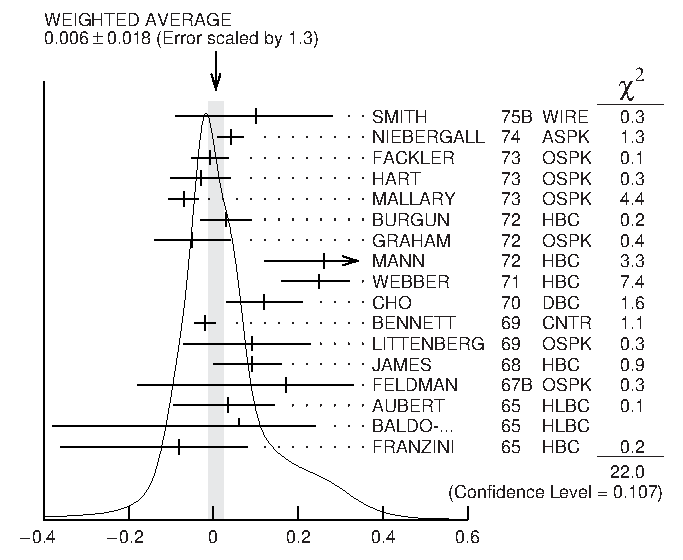
\includegraphics{filename} %multiple includegraphics may be used, 
	% with usual \hfill and \\ newline structures. 
\end{pdgxfigure}
\end{verbtex}

Figures placed in the \invt{figures} directory will be automaticallly found. 
Option keys may also be passed to individual \lstinline{\includegraphics} commands,  
as usual, if separate control is desired of multiple \lstinline{\includegraphics} in the same \invt{pdgxfigure} environment.
I.e. \lstinline!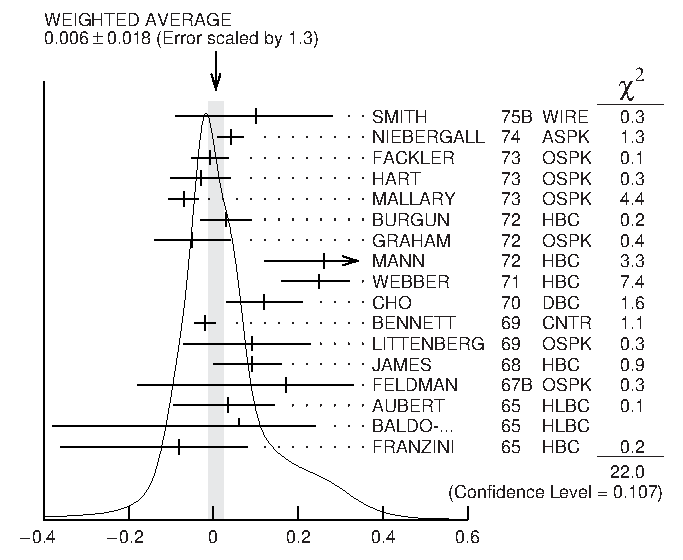
\includegraphics[<option keys>]{filename}!.

\Isubsection{Float scaling and width keys}
\label{sec:ginkeys}
As in the usual implementation of the \invt{graphicx} package, the \lstinline{\includegraphics} command takes optional standard keys \invt{width = ...}, \invt{scale = ...}.
which are used to control the width or scale of the bounding box. 
We use the same key structure to pass options to the \invt{pdgxfigure} environment, as well as to the \invt{pdgxtable} environment (see Sec.~\ref{sec:tables}).

The version specific keys \lstinline!<version>width! and \lstinline!<version>scale! have been added, 
that implement width or scaling choices only in the specific \invt{<version>}.
One may use these keys in concert with the usual \invt{width} and \invt{scale} keys, with the caveat that the order of keys matters: 
Keys are read left to right, and rightwards keys typically override leftwards ones. 
For example, passing the option keys (to either \invt{pdgxfigure} or \invt{pdgxtable}, or \lstinline{\includegraphics})
\begin{verbtex}
	[width=0.8\linewidth, bookwidth=0.9\linewidth]
\end{verbtex}
implements the \invt{width} key setting except in the book version. 
The option \lstinline!bookwidth=0.9\linewidth! followed by
\lstinline!width=0.8\linewidth! would instead implement only the version-general \lstinline!width=0.8\linewidth! setting.

\textbf{Note:} Because of specialization of the \invt{graphicx} key structure in the PDG class,
to use a \invt{scale} or \invt{<version>scale} key in an \lstinline{\includegraphics} command or \invt{pdgxfigure} environment
one must first pass an option key \invt{width=!}. This is not required for  \invt{pdgxtable}.

An additional key \lstinline!<version>bbscale! scales the float bounding box.
For some overwide floats that are larger than the nominal page width---in particular, overwide tables, see Sec.~\ref{sec:tables}---simply 
rescaling down the float does not allow it to be properly aligned on the page.
This key can be increased above $1$ (the default), to provide a sufficiently large bounding box for the float, that may then be scaled down to size with correct alignment.

\Isubsection{Available keys for \invt{pdgxfigure}}
Following is a list of available optional keys for \invt{pdgxfigure}, and default settings if not invoked.
As usual, keys are evaluated left to right. 
The version-general \invt{width} key can be used (and will override any preceeding version-specfic width key).
\begin{itemize}
	\item \invt{place}: Takes any combination of \invt{h}, \invt{t}, \invt{b}, \invt{p} (with optional \invt{\!}) that specifies float placement. Default is \invt{\!ht}.
	\item \invt{wide}: Takes \invt{true} or \invt{false} to specify the figure as full page width in either single or two column mode. Default is \invt{false}.
	\item \invt{width} or \invt{<version>width}: Sets the global or version specific width of the figure bounding box, respectively. Default is 0.75 of the line width (or text width, for wide figures).
	\item \invt{scale} or \invt{<version>scale}: Scales the figure according to float value passed to the key. 
	The option \lstinline{width=!} must be passed to turn off default width behavior and enable scaling keys.
\end{itemize}

\Isubsection{Examples}
The following produces a default-style, shown in Figure~\ref{examples:fig:example}. 
We recommend including the file extension in the \lstinline{\includegraphics} argument, to assist our editorial staff in addressing any figure quality problems.
\begin{verbtex}
\begin{pdgxfigure}[place=t] 
	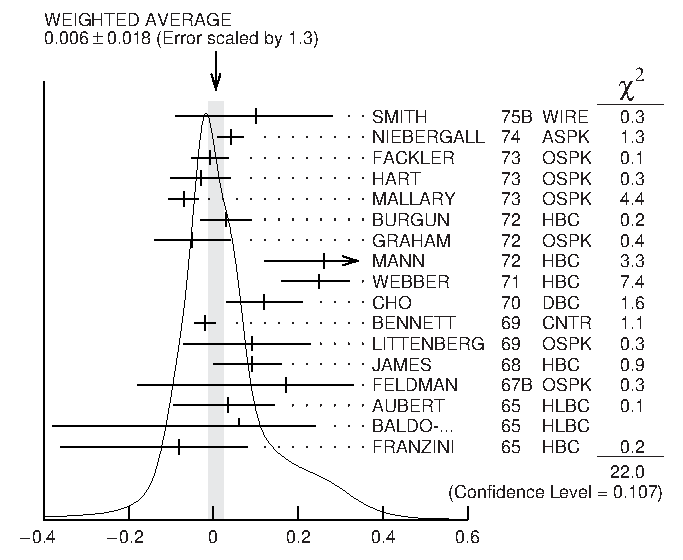
\includegraphics{filename.pdf}
	\caption{Example default figure}
	\label{examples:fig:example}
\end{pdgxfigure}
\end{verbtex}
\begin{pdgxfigure}[place=t]
	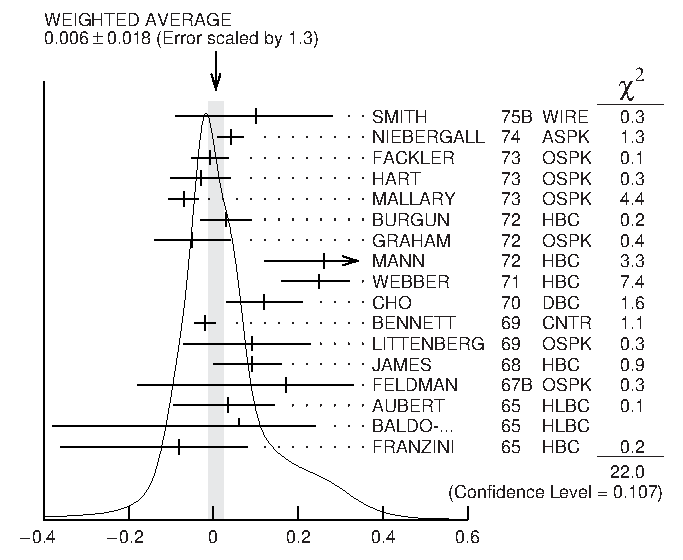
\includegraphics{filename.pdf}
	\caption{Example default figure}
	\label{examples:fig:example}
\end{pdgxfigure}

A double wide figure, shown in Fig.~\ref{examples:fig:example2}:
\begin{verbtex}
\begin{pdgxfigure}[wide=true,place=h, webwidth=0.45\linewidth, 
		bookwidth=0.9\linewidth] 
	%width key applies to all includegraphics instances
	%compiling in different versions will produce different widths
	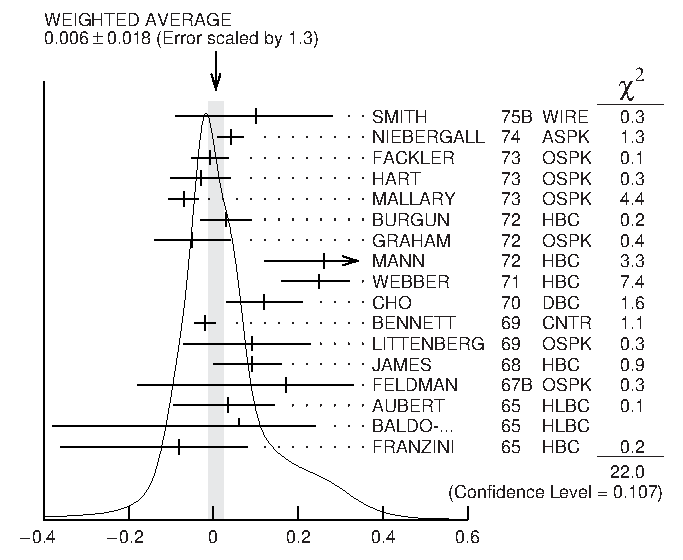
\includegraphics{filename.pdf}\hfill
	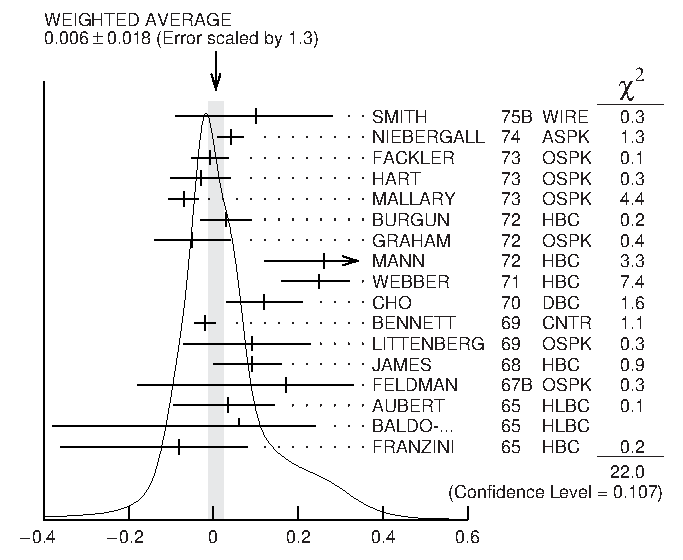
\includegraphics{filename.pdf}
	\caption{Example double wide figure, 
		with different book and web versions}
	\label{examples:fig:example2}
\end{pdgxfigure}
\end{verbtex}
\begin{pdgxfigure}[wide=true,place=h,width=0.45\textwidth] 
	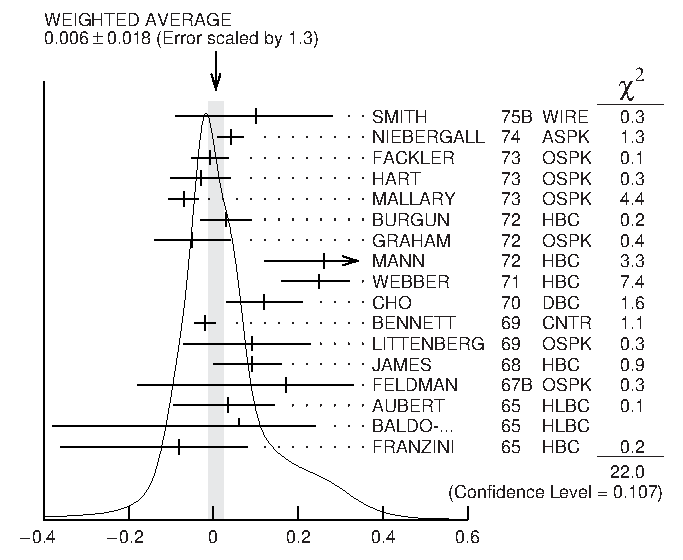
\includegraphics{filename.pdf}\hfill
	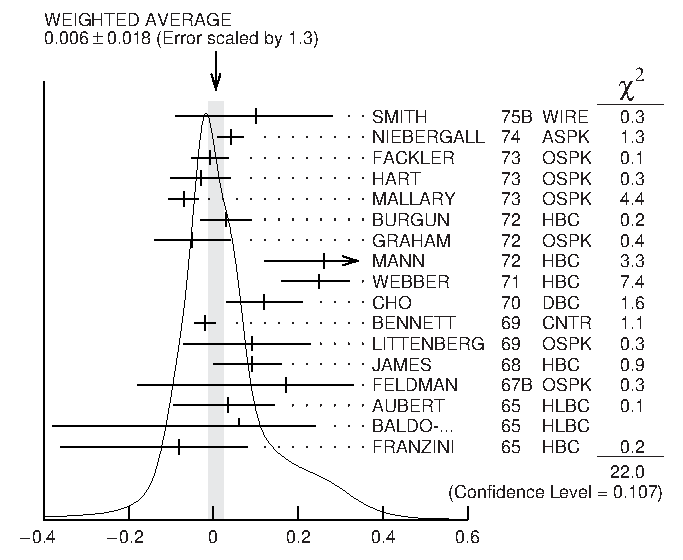
\includegraphics{filename.pdf}
	\caption{Example double wide figure, with different book and web versions}
	\label{examples:fig:example2}
\end{pdgxfigure}

A double wide figure with separate option and scaling keys, shown in Fig.~\ref{examples:fig:example3}:
\begin{verbtex}
\begin{pdgxfigure}[wide=true,place=h,width = 0.3\linewidth] 
	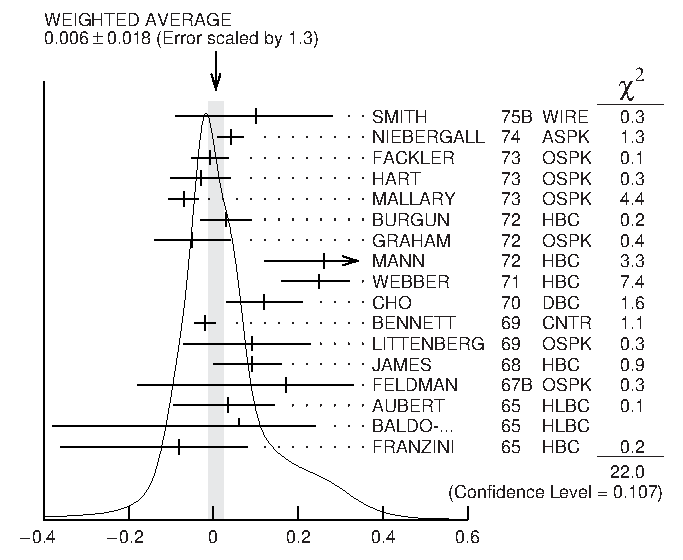
\includegraphics{filename.pdf}\hspace{1cm}
	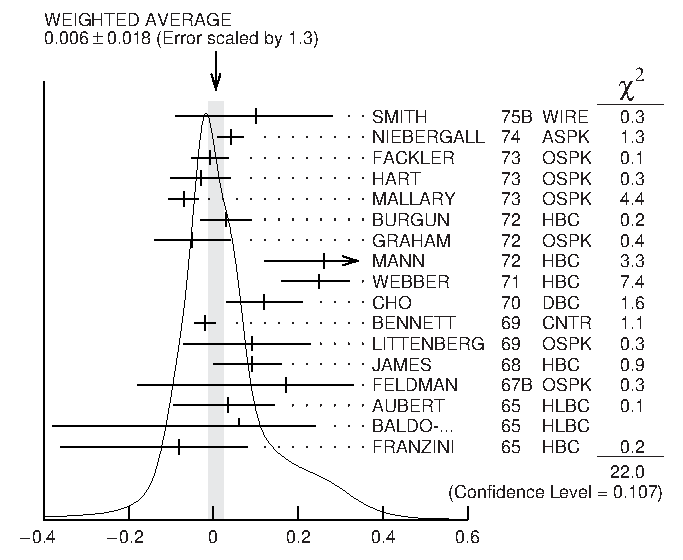
\includegraphics[width = !,scale =0.3,angle = 90]{filename}
	\caption{Example double figure, 
		with separate option and scaling keys, in both book and web versions}
	\label{examples:fig:example3}
\end{pdgxfigure}
\end{verbtex}
\begin{pdgxfigure}[wide=true,place=h,width = 0.3\linewidth] 
	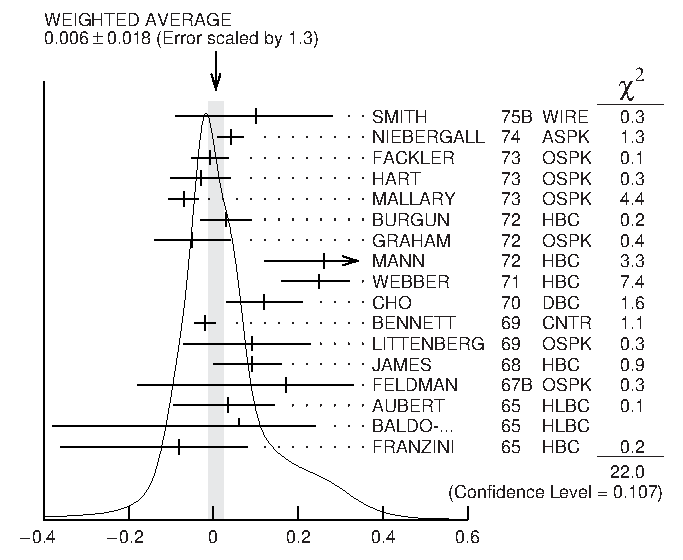
\includegraphics{filename.pdf}\hspace{1cm}
	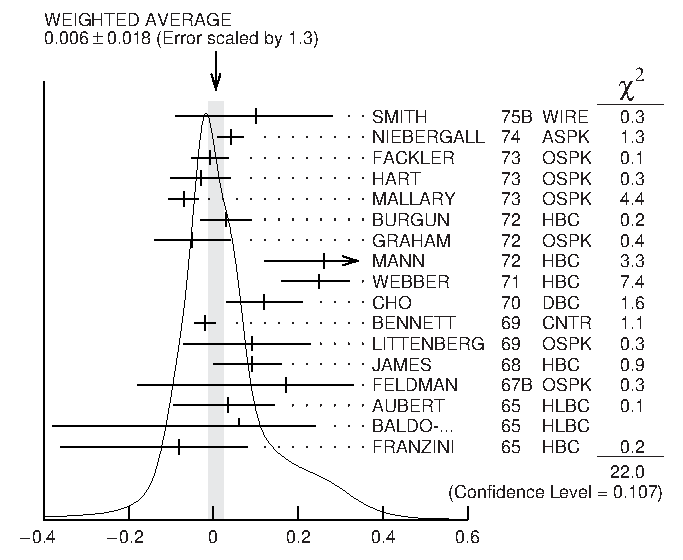
\includegraphics[width = !,scale =0.3,angle = 90]{filename}
	\caption{Example double wide figure, with separate option and scaling keys, in both book and web versions}
	\label{examples:fig:example3}
\end{pdgxfigure}

\Isubsection{\invt{pdgfigure} commands}
To add a figure, one may also use the \lstinline{\pdgfigure} or \lstinline{\pdgwidefigure} commands 
to typeset a single-column figure or double-column wide figure (for the book version), respectively. 
To include two images in one figure one may use \lstinline{\pdgdoublefigure}.
These commands are less powerful than \invt{pdgxfigure}, but automatically incorporate all PDG styles.

The macros \lstinline{\pdgfigure} and \lstinline{\pdgwidefigure} take the following arguments:
\begin{verbtex}
	\pdgfigure{<filename>}
	{<caption>}{<label>}{<placement options>}
	{<other option keys>}
\end{verbtex}
\vspace{-10pt}
while the macro \lstinline{\pdgdoublefigure} takes the following arguments:
\begin{verbtex}
	\pdgdoublefigure{<filename1>}{<filename2>}
	{<caption>}{<label>}{<placement options>}
	{<other option keys>}
\end{verbtex}
Some examples of the \invt{pdgfigure} commands are shown in Figs.~\ref{examples:fig:ideogram1}, \ref{examples:fig:ideogram2} and \ref{examples:fig:ideogram3}, respectively:
\begin{verbtex}
	\pdgfigure{filename.pdf}{Figure with caption and label}
	{examples:fig:ideogram1}{ht!}{}
	
	\pdgdoublefigure{filename.pdf}{filename.pdf}
	{Two figures, with caption and label, reduced in size}
	{examples:fig:ideogram2}{ht!}{width=0.3\textwidth}
	
	\pdgwidefigure{filename.pdf}{Wide figure}
	{examples:fig:ideogram3}{t}{}
\end{verbtex}
\FloatBarrier
\pdgfigure{filename.pdf}{Figure with caption and label}{examples:fig:ideogram1}{ht!}{}
\pdgdoublefigure{filename.pdf}{filename.pdf}{Two figures, with caption and label, reduced in size}{examples:fig:ideogram2}{ht!}{width=0.3\textwidth}
\pdgwidefigure{filename.pdf}{Wide figure}{examples:fig:ideogram3}{t}{}
\FloatBarrier

\Isection{Tables}
\label{sec:tables}
\Isubsection{ \invt{pdgxtable} and \invt{pdgxtabular}}
The PDG class provides multipurpose table and tabular environments, \invt{pdgxtable} and \invt{pdgxtabular}. 
These operate similarly to the standard \invt{table} and \invt{tabular} environments: \invt{(pdgx)table} creates a floating environment, 
while \invt{(pdgx)tabular} creates the actual tabulated display. 

The \lstinline!\caption! and \lstinline!\label! commands may be used as in the usual \invt{table} environment.
\textbf{Note: A table caption should be placed above the table.}
In addition, \invt{pdgxtable} takes a wide array of additional option keys that implement features and formatting of the prior PDG table commands/environments.  
These include keys that control placement, multicolumn spanning, version-specific widths and scaling (see Sec.~\ref{sec:ginkeys}), rotation, stretching, and caption widths.
The generic usage is
\begin{verbtex}
\begin{pdgxtable}[<option keys>]
	\caption{This is a PDG table}
	\label{tab:label}
	\begin{pdgxtabular}{<column settings>} % the usual c, l, r, | etc
		\pdgtableheader{...} %column header & separated entries go here
		%table & separated entries go here
	\end{pdgxtabular}
	%multiple pdgtabular environments are allowed
\end{pdgxtable}
\end{verbtex}

As for the usual \invt{table} environment, one may include multiple \invt{pdgxtabular}s in a single \invt{pdgxtable}.
While the \invt{pdgxtable} environment has default handling for caption widths in wide and regular tables, for both book and web versions, 
absolute control of the caption width can be implmented with a \lstinline{\captionsetup} command inside the \invt{pdgxtable} environment. 
For example \lstinline!\captionsetup{width=\linewidth}! gives a full width caption.

\Isubsection{Available keys for \invt{pdgxtable}}
Following is a list of available optional keys, and default settings if not invoked.
As usual, keys are evaluated left to right. 
While, the version-general \invt{width} key can be used (and will override any preceeding version-specfic width key), 
there is no version-general \invt{scale} key. 
Scaling of the tables is best done with the \invt{<version>scale} keys.

\begin{itemize}
	\item \invt{place}: Takes any combination of \invt{h}, \invt{t}, \invt{b}, \invt{p} (with optional \invt{\!}) that specifies float placement. Default is \invt{\!ht}.
	\item \invt{wide}: Takes \invt{true} or \invt{false} to specify the table as full page width in either single or two column mode. Default is \invt{false}.
	\item \invt{width} or \invt{<version>width}: Sets the version specific maximum width of the table bounding box. 
	Default is the maximum text width implied by the \invt{wide} key setting.
	Width settings exceeding this default are ineffective. Footnotes are scaled, but caption width is not affected.
	\item \invt{<version>scale}: Scales the table according to float value passed to the key. 
	For overwide tables, there is always a value $<1$ at which the table will be properly set to maximum page width.
	Footnotes are scaled, but caption width is not affected. Note the global \invt{scale} is disabled for \invt{pdgxtable}.
	\item \invt{<version>bbscale}: Scales the bounding box of the table. 
	For some overwide tables that are larger than the nominal page width, simply rescaling down the table does not allow the table to be properly aligned on the page.
	This key can be increased above $1$ (the default), to provide a sufficiently large bounding box for the table, that may then be scaled down to size with correct alignment.
	\item \invt{widecaptionscale}: For \invt{wide = true} tables, scales the caption width with respect to the maximum page width. Default is $0.75$.
	\item \invt{narrowcaptionscale}: For \invt{wide = false} or default tables, scales the caption width with respect to the maximum column width. Default is $0.9$.
	\item \invt{rotated}: Takes \invt{left} or \invt{right} to rotate the table, but not the caption, $90^\circ$ anticlockwise or clockwise, respectively. 
	The caption may be rotated independently, as needed with a \lstinline{\rotatebox}.
	\item \invt{sideways}: Takes \invt{true} or \invt{false} to rotate the table, including the caption, $90^\circ$ anticlockwise or clockwise, 
	according to whether the page number is even or odd.
	In a sideways table, other key width and scaling settings are still effective, but scale with respect to the page height. 
\end{itemize}


\Isubsection{Examples}
Some (simple) examples of \invt{pdgxtable} can be found in Table~\ref{examples:tab:styles} and Sec~\ref{sec:macros}.
For example, Tab.~\ref{examples:tab:styles} is typeset as
\begin{verbtex}
\begin{pdgxtable}[place=h,bookscale = 0.9,bookbbscale=2]
	\caption{Styles for the different typesetting versions}
	\label{examples:tab:styles}
	\begin{pdgxtabular}{ccccc}
		Version 		& Columns  & Font size 	& Helper Tags\footnote{
			Tags for each equation, table, figure, and bibliography entry 
			are displayed in margin or interspaced} & Line numbers\\
		\hline
		draft	& 1		   & 11pt		& Yes & Yes \\
		...
	\end{pdgxtabular}
\end{pdgxtable}
\end{verbtex}

Tables~\ref{examples:tab:commu} and~\ref{examples:tab:commp} are typeset as a two \invt{pdgxtabular}s in a single \invt{pdgxtable}, via
\begin{verbtex}
\begin{pdgxtable}[wide=true, place=!ht, webscale = 0.8]
	\caption{Common units}
	\label{examples:tab:commu}
	\begin{pdgxtabular}{lr | lr | lr}
		\showsymbol{\TeV} &  \showsymbol{\syin} & \showsymbol{\barn}   \\
		...
	\end{pdgxtabular}
	\caption{Common particles}
	\label{examples:tab:commp}
	\begin{pdgxtabular}{lr | lr | lr}
   		\showsymbol{\pp} &  \showsymbol{\ee} & \showsymbol{\pizero}   \\
  		...
	\end{pdgxtabular}
\end{pdgxtable}
\end{verbtex}

\Isubsection{Common problems and recommendations}
The \invt{pdgxtabular} environment is capable of handling the usual \lstinline{\multicolumn} and \lstinline{\multirow} objects, 
that allow for more complicated tables with cells spanning multiple rows and/or columns. 
We recommend avoiding use of \lstinline{\multispan}. 
For multiline cells, the \lstinline{\makecell} command from the \invt{makecell} package is recommended.

\Isection{Labels and referencing}
\label{sec:labels}

\Isubsection{Style guide}
As usual, the \lstinline{\label} and \lstinline{\ref} commands (and their derivatives) may be used to reference equations, tables, figures, and so on. 
To permit easy cross-referencing throughout the entire review, we request that you use the following labelling convention: \invt{BASENAME:type:name}
with \invt{type} corresponding to one of the following options
\begin{itemize}
\item {\tt fig} for figures
\item {\tt eq } for equation
\item {\tt tab} for tables
\item {\tt sec} for section, subsection etc..
\item {\tt foot} for footnotes.
\end{itemize}

\Isubsection{Missing references}

In default LaTeX, missing references are typically typeset as ``\textbf{??}''. 
To improve the typesetting experience, the \lstinline{\ref} command has been modified in the PDG class so that missing reference keys are printed out explicitly: 
For instance, a \lstinline!\ref{eqn:name}! that references a missing label called \invt{eqn:name}, will display as \ref{eqn:name}.
Similarly, the \lstinline{\cite} command will explicitly print out missing citation references. E.g. 
a \lstinline!\cite{name:2021ab}! that references a missing label called \invt{name:2021ab}, will display as \cite{name:2021ab}

\Isubsection{Cross-review referencing}
It is occasionally necessary or useful to reference (sub)sections, equations, figures, tables and so on belonging to other reviews or other reviews themselves. 
\textbf{Note:} Please use the \lstinline{\crossref} command for cross-review referencing.

Implementing a cross-reference to another review requires knowledge of its  \invt{BASENAME}:  
You must use the \invt{BASENAME} associated with the target review, not the \invt{BASENAME} of the review you're currently working on. 
To identify the  \invt{BASENAME} of another review, login into the \href{https://pdgworkspace.lbl.gov/Reviews.action}{PDG Workspace} (click to be redirected). 
Under \emph{Reviews} select from the drop-down menu \emph{All reviews}. 
Click on the title of the review you are interested in, and then select the \emph{Technical details} tab. 
The \invt{BASENAME} is the first entry.


If the full \invt{BASENAME:type:name} reference is known, you may include it with the usage \\
\lstinline!\crossref{BASENAME:type:name}!. 
This will typeset in your document as ``\crossref{BASENAME:type:name}'', because your local auxiliary files do not have the reference information of the other review.
PDG editorial staff will implement the cross-reference properly, when your review is prepared for production.

If the \invt{BASENAME:type:name} reference is not known, or the authors of the other review did not label the obect that you wish to reference, 
you may instead provide any descriptive argument to \lstinline{\crossref}. 
For example, \lstinline!\crossref{Equation 34.1.10}!.  
PDG editorial staff will implement the cross-reference properly, when your review and the other review are prepared for production.

\Isubsection{Booklet labeling and referencing}
If your review has a booklet version, it needs to be prepared at the same time as you prepare your full review.
The content to be displayed in the booklet needs to be included in \invt{BASENAME-booklet.tex}. 

The numerical tags for equations, tables, and figures in the booklet version of a review should match the tags in the full version. 
This can be achieved automatically in the booklet version by using a \lstinline!\tag{\ref{BASENAME:type:name}}! construction instead of \lstinline{\label}
to refer to the reference in the full version.
For example, if the full version has a labelled equation
\begin{verbtex}
\begin{equation}
	\label{BASENAME:eq:name}
	...
\end{equation}
\end{verbtex}
then including in \invt{BASENAME-booklet.tex}
\begin{verbtex}
\begin{equation}
	\tag{\ref{BASENAME:eq:name}}
	...
\end{equation}
\end{verbtex}
will automatically label the equation correctly. 
To achieve the same result for figures and tables, one may place in the booklet version
\begin{verbtex}
	\renewcommand{\thetable}{\ref{BASENAME:type:name}}
	\renewcommand{\thefigure}{\ref{BASENAME:type:name}}
\end{verbtex}
before each table or figure environment, respectively. 


\Isection{Index entries}
\label{sec:index}

Review authors should think about any keywords that should be included into the index of the Review of Particle Physics. PDG uses the standard \LaTeX\  \invt{makeidx} package. Thus an entry ``sample text'' can be added to the index by placing
\begin{verbtex}
\index{sample text}
\end{verbtex}
at the appropriate place in the source file. Formatting of entries with Greek letters or math symbols as well as subentries are also supported. For example
\begin{verbtex}
\index{sigma@$\$$\sigma$\$$} 
\end{verbtex}
creates an index entry $\sigma$ in the proper alphabetical order, while
\begin{verbtex}
\index{Searches!Axion searches} 
\end{verbtex}
produces a subentry ``Axion searches'' under the ``Searches'' index entry.

All index entries defined in a given review will be shown on the last page when the draft version is made. PDG staff will standardize all index entries during the final processing of all reviews. Therefore what matters is not the final formatting of index entries but that all relevant entries are added in the correct place.


\Isection{Bibliography}
\label{sec:cites}

Citations are handled using BibTeX. To add a citation to your review:
\begin{itemize}
\item Look up the reference in INSPIRE and download its BibTeX entry (see bottom of the \emph{Information} tab for the article, under \emph{Export}).
\item Add the BibTeX entry to the \invt{BASENAME.bib} file. Note the article tag assigned by INSPIRE: You can see it in the first line of the BibTeX entry, after \lstinline!@article{!.
\item Cite the reference with \lstinline{\cite}, using the article tag assigned by INSPIRE.
\end{itemize}

For example, to add a reference to the Review of Particle Physics (2018) 
add the following code to \invt{BASENAME.bib}:
\begin{verbtex}
@article{Tanabashi:2018oca,
      author         = "Tanabashi, M. and others",
      title          = "{Review of Particle Physics}",
      collaboration  = "Particle Data Group",
      journal        = "Phys. Rev.",
      volume         = "D98",
      year           = "2018",
      number         = "3",
      pages          = "030001",
      doi            = "10.1103/PhysRevD.98.030001",
      SLACcitation   = "%%CITATION = PHRVA,D98,030001;%%"
 }
\end{verbtex}
and then one may add a reference to it in \invt{BASENAME-main.tex} via \lstinline!\cite{Tanabashi:2018oca}!.

If a BibTeX entry downloaded from INSPIRE does not render correctly, 
you should first make sure you have the latest PDG style files, by running \invt{svn update} (after committing any edits you have made).
If this doesn't fix the issue please contact \invt{latexsupport@pdg.lbl.gov} for advice.  
If it appears, however, to be simply a mistake in INSPIRE's entry, 
rename the label to the form \invt{BASENAME:<INSPIRE label>} and then edit the entry as needed.
\textbf{Please do not edit entries downloaded from INSPIRE without changing the label.}
Changing the label will permit PDG editorial staff to easily identify and track edited citations, as well as notify INSPIRE of required corrections.
In case the reference does not appear in INSPIRE at all, please also use the convention for the label: \invt{BASENAME:name}.

Multiple references can be added to a single set of brackets with \lstinline!\cite{cite-key-1,cite-key-2,...}!.
One may group multiple references into the same numerical citation tag, using a \invt{*} prefix on subsequent citation keys: For example \lstinline!\cite{cite-key-1,*cite-key-2,*cite-key-3}!.
If a paper citation key is preceded by the asterisk, it can't be cited separately later, and doing so will result in a compilation error.
We recommend citing papers individually, without using the asterisk to group them.


\Isection{Footnotes}
Footnote styles are standardized throughout the review. In (rare) cases that the style needs to be changed, this is achieved via \lstinline!\setfootnotestyle{<style>}!,
where \invt{<style>} can be \lstinline{\fnsymbol} or \lstinline{\alph}, \lstinline{\Alph}, \lstinline{\arabic}, \lstinline{\roman}, \lstinline{\Roman} etc.

Sometimes the \LaTeX \ engine miscalculates the amount of space required for a footnote, resulting in overprinting of the footer.
One can help the engine obtain a better estimate by adjusting the effective page size. 
This can be done by placing \lstinline!\enlargethispage{-2\baselineskip}! somewhere just before the \lstinline{\footnote}; the \invt{-2} may be changed to any number. 

\Isection{Miscellaneous control commands}

\Isubsection{Unbalanced last page}
In the book version, the columns of the final page are automatically balanced. 
If this behavior is undesired, it may be altered by invoking \lstinline!\balancedlastpagefalse!.
The invocation may be added anywhere in the document.

\Isubsection{Blank last page}
In the book version, a blank final page may be added via \lstinline!\blankendpagetrue!.
The invocation may be added anywhere in the document.

\Isubsection{Book-only reviews}
Certain reviews are typeset for the web using the book version formatting. 
This is enforced automatically within the PDG system by \lstinline!\def\iswebbook{1}! before the \lstinline{\documentclass} invocation. 
The draft version, however, for such reviews are typeset in the usual draft/web format.

\clearpage
\Isection{PDG Macros}
\label{sec:macros}

\begin{pdgxtable}[wide=true, place=!ht, webscale = 0.8]
	\vspace{-10pt}
	\caption{Common units}
	\label{examples:tab:commu}
	\begin{pdgxtabular}{lr | lr | lr}
		\showsymbol{\TeV     } &  \showsymbol{\syin} & \showsymbol{\barn     }   \\
		\showsymbol{\MeV     } &  \showsymbol{\inch} & \showsymbol{\mbarn    }   \\
		\showsymbol{\keV     } &  \showsymbol{\ft  } & \showsymbol{\microbarn}   \\
		\showsymbol{\eV      } &  \showsymbol{\km  } & \showsymbol{\nb       }   \\
		\showsymbol{\GeVc    } &  \showsymbol{\m   } & \showsymbol{\pb       }   \\
		\showsymbol{\GeVcSq  } &  \showsymbol{\cm  } & \showsymbol{\fb       }   \\
		\showsymbol{\GeVcc   } &  \showsymbol{\mm  } & \showsymbol{\invnb    }   \\
		\showsymbol{\GeVccSq } &  \showsymbol{\mum } & \showsymbol{\invpb    }   \\
		\showsymbol{\MeVc    } &  \showsymbol{\nm  } & \showsymbol{\invfb    }   \\
		\showsymbol{\MeVcc   } &  \showsymbol{\fm  } & \showsymbol{\invab    }   \\
		\showsymbol{\invps   } &  \showsymbol{\nm  } & \showsymbol{\lum      }   \\
			&&  \showsymbol{\ma  } &&  \\
		\showsymbol{\degr    }  &  \showsymbol{\cma } && \\
			&&  \showsymbol{\mma } &&   \\
			&&  \showsymbol{\muma} &&   \\
	\end{pdgxtabular}
	\vspace{10pt}
	\caption{Common particles}
	\label{examples:tab:commp}
	\vspace{-10pt}
	\begin{pdgxtabular}{lr | lr | lr}
   \showsymbol{\pp         } &  \showsymbol{\ee           } & \showsymbol{\pizero   }   \\
   \showsymbol{\pbar       } &  \showsymbol{\epm          } & \showsymbol{\piplus   }   \\
   \showsymbol{\ppbar      } &  \showsymbol{\epem         } & \showsymbol{\piminus  }   \\
   \showsymbol{\tbar       } &  \showsymbol{\en           } & \showsymbol{\pipm     }   \\
   \showsymbol{\ttbar      } &  \showsymbol{\ep           } & \showsymbol{\pimp     }   \\
   \showsymbol{\bbar       } &  \showsymbol{\mumu         } & \showsymbol{\etaprime }   \\
   \showsymbol{\bbbar      } &  \showsymbol{\mun          } & \showsymbol{\Kzero    }   \\
   \showsymbol{\cbar       } &  \showsymbol{\mup          } & \showsymbol{\Kzerobar }   \\
   \showsymbol{\ccbar      } &  \showsymbol{\tautau       } & \showsymbol{\kaon     }   \\
   \showsymbol{\sbar       } &  \showsymbol{\taup         } & \showsymbol{\Kplus    }   \\
   \showsymbol{\ssbar      } &  \showsymbol{\taum         } & \showsymbol{\Kminus   }   \\
   \showsymbol{\ubar       } &  \showsymbol{\lepton       } & \showsymbol{\KzeroL   }   \\
   \showsymbol{\uubar      } &  \showsymbol{\leptonm      } & \showsymbol{\Kzerol   }   \\
   \showsymbol{\dbar       } &  \showsymbol{\ellm         } & \showsymbol{\Klong    }   \\
   \showsymbol{\ddbar      } &  \showsymbol{\leptonp      } & \showsymbol{\KzeroS   }   \\
   \showsymbol{\fbar       } &  \showsymbol{\ellp         } & \showsymbol{\Kzeros   }   \\
   \showsymbol{\ffbar      } &  \showsymbol{\leptonlepton } & \showsymbol{\Kshort   }   \\
   \showsymbol{\qbar       } &  \showsymbol{\ellell       } & \showsymbol{\Kstar    }   \\
   \showsymbol{\qqbar      } &  \showsymbol{\enu          } & \showsymbol{\jpsi     }   \\
   \showsymbol{\nbar       } &  \showsymbol{\munu         } & \showsymbol{\Jpsi     }   \\
   \showsymbol{\nnbar      } &  \showsymbol{\taunu        } & \showsymbol{\psip     }   \\
   \showsymbol{\neutron    } &  \showsymbol{\lnu          } & \showsymbol{\chic     }   \\
   \showsymbol{\antineutron} &  \showsymbol{\nub          } & \showsymbol{\UoneS    }   \\
   \showsymbol{\deuteron   } &  \showsymbol{\nunub        } & \showsymbol{\chib     }   \\
   \showsymbol{\Zzero      } &  \showsymbol{\nue          } & \showsymbol{\Dstar    }   \\
   \showsymbol{\Zboson     } &  \showsymbol{\nueb         } & \showsymbol{\Bd       }   \\
   \showsymbol{\Wplus      } &  \showsymbol{\nuenueb      } & \showsymbol{\Bs       }   \\
   \showsymbol{\Wminus	   } &  \showsymbol{\num          } & \showsymbol{\Bu       }   \\
   \showsymbol{\Wboson	   } &  \showsymbol{\numb         } & \showsymbol{\Bc       }   \\ 
   \showsymbol{\Wpm   	   } &  \showsymbol{\numnumb      } & \showsymbol{\Lb       }   \\
   \showsymbol{\Wmp        } &  \showsymbol{\nut          } & \showsymbol{\Bstar    }   \\
   \showsymbol{\Hzero } &  \showsymbol{\nutb         } & \showsymbol{\BoBo     }   \\
   \showsymbol{\Hboson}  &	\showsymbol{\nutnutb      } & \showsymbol{\BodBod   }    \\		    
   \showsymbol{            } &	\showsymbol{              } & \showsymbol{\BosBos   }    \\		    
   \showsymbol{            } &	\showsymbol{              } & \showsymbol{\LambdaStar}  \\
	\end{pdgxtabular}
\end{pdgxtable}

\begin{pdgxtable}[wide=true, place=h, webscale = 0.8]
	\caption{Hypothetical particles}
	\begin{pdgxtabular}{lr | lr | lr}
   \showsymbol{\Azero }      &  \showsymbol{\gravino   } & \showsymbol{\slepton   }   \\
   \showsymbol{\hzero }      &  \showsymbol{\Zprime    } & \showsymbol{\sleptonL  }   \\
   \showsymbol{\Hzero }      &  \showsymbol{\Zstar     } & \showsymbol{\sleptonR  }   \\
   \showsymbol{\Hplus }  	  &  \showsymbol{\squark    } & \showsymbol{\sel       }   \\
   \showsymbol{\Hminus}       &  \showsymbol{\squarkL   } & \showsymbol{\selL      }   \\
   \showsymbol{\Hpm   }   	&  \showsymbol{\squarkR   } & \showsymbol{\selR      }   \\
   \showsymbol{\Hmp   }       &  \showsymbol{\gluino    } & \showsymbol{\smu       }   \\
   \showsymbol{\ggino }     &  \showsymbol{\stop      } & \showsymbol{\smuL      }   \\
   \showsymbol{\chinop}      &  \showsymbol{\stopone   } & \showsymbol{\smuR      }   \\
   \showsymbol{\chinom}      &  \showsymbol{\stoptwo   } & \showsymbol{\stau      }   \\
   \showsymbol{\chinopm}      &  \showsymbol{\stopL     } & \showsymbol{\stauL     }   \\
   \showsymbol{\chinomp}     &  \showsymbol{\stopR     } & \showsymbol{\stauR     }   \\
   \showsymbol{\chinoonep}     &  \showsymbol{\sbottom   } & \showsymbol{\stauone   }   \\
   \showsymbol{\chinoonem}   &  \showsymbol{\sbottomone} & \showsymbol{\stautwo   }   \\
   \showsymbol{\chinoonepm}   &  \showsymbol{\sbottomtwo} & \showsymbol{\snu       }   \\
   \showsymbol{\chinotwop}  &  \showsymbol{\sbottomL  } & \showsymbol{           }   \\
   \showsymbol{\chinotwom}   &  \showsymbol{\sbottomR  } & \showsymbol{           }   \\
   \showsymbol{\chinotwopm}   &  \showsymbol{           } & \showsymbol{           }   \\
   \showsymbol{\nino}  &  \showsymbol{           } & \showsymbol{           }   \\
   \showsymbol{\ninoone}        &  \showsymbol{           } & \showsymbol{           }   \\
   \showsymbol{\ninotwo}     &  \showsymbol{           } & \showsymbol{           }   \\
   \showsymbol{\ninothree}     &  \showsymbol{           } & \showsymbol{           }   \\
   \showsymbol{\ninofour}   &  \showsymbol{           } & \showsymbol{           }   \\
	\end{pdgxtabular}
\vspace*{10pt}
	\caption{Useful symbols for proton-proton physics}
\vspace*{-10pt}	
	\begin{pdgxtabular}{lr | lr }
   \showsymbol{\pT  }      &  \showsymbol{\rts }   \\
   \showsymbol{\pt  }      &  \showsymbol{\sqs } \\
   \showsymbol{\ET  }      &  \showsymbol{\mh}  \\
   \showsymbol{\eT  }      &  \showsymbol{\mW}  \\
   \showsymbol{\et  }      & \showsymbol{\mZ}   \\
   \showsymbol{\HT  }      & \showsymbol{\mH}   \\
   \showsymbol{\pTsq}      &&   \\
   \showsymbol{\MET }      &&   \\
   \showsymbol{\met }      &&   \\
   \showsymbol{\Ecm }      &&   \\
	\end{pdgxtabular}
\vspace*{10pt}
	\caption{Monte Carlo Generators}
\vspace*{-10pt}		
	\begin{pdgxtabular}{lr | lr | lr}	
   \showsymbol{\ACERMC    }      &  \showsymbol{\MCatNLO   } & \showsymbol{\Comphep    }   \\
   \showsymbol{\ALPGEN    }      &  \showsymbol{\AMCatNLO  } & \showsymbol{\Prospino   }   \\
   \showsymbol{\GEANT     }      &  \showsymbol{\MCFM      } & \showsymbol{\LO         }   \\
   \showsymbol{\Herwigpp  }      &  \showsymbol{\METOP     } & \showsymbol{\NLO        }   \\
   \showsymbol{\HERWIGpp  }      &  \showsymbol{\POWHEG    } & \showsymbol{\NLL        }   \\
   \showsymbol{\Herwig    }      &  \showsymbol{\POWHEGBOX } & \showsymbol{\NNLO       }   \\
   \showsymbol{\HERWIG    }      &  \showsymbol{\POWPYTHIA } & \showsymbol{\muF        }   \\
   \showsymbol{\JIMMY     }      &  \showsymbol{\PROTOS    } & \showsymbol{\muR        }   \\
   \showsymbol{\MADSPIN   }      &  \showsymbol{\PYTHIA    } & \showsymbol{            }   \\
   \showsymbol{\MADGRAPH  }      &  \showsymbol{\SHERPA    } & \showsymbol{            }   \\
   \showsymbol{\MGMCatNLO }      &  \showsymbol{           } & \showsymbol{            }   \\
	\end{pdgxtabular}
\end{pdgxtable}

\Isection{Tables: Legacy commands}

Though no longer recommended, legacy \lstinline{\pdgtable} or \lstinline{\pdgwidetable} commands 
to typeset a single-column table or double-column wide table (for the book version), respectively.
The \lstinline{\pdgtableheader} macro may be used in the first line of the table to automatically typeset a header.

The macros \lstinline{\pdgtable} and \lstinline{\pdgwidetable} take the following arguments:
\begin{verbtex}
	\pdgtable{<column styles>}
	{<caption>}{<label>}{<option keys>}
\end{verbtex}
Some examples usages of these commands follow, in Tables~\ref{examples:tab:table1}, \ref{examples:tab:table2} and~\ref{examples:tab:table3} below.
\begin{verbtex}
\begin{pdgtable}{c c c} 
	{Table}{examples:tab:table1}{h!}
	\pdgtableheader{ Column 1 & Column 2 & Column 3}
	row1  & 1  & 2\\
	row2  & 1  & 2\\
	row3  & 1  & 2\\
\end{pdgtable}
\end{verbtex}   
\begin{verbtex}
\begin{pdgtable}{|c | c | c | c|} 
	{Multicolumn table}{examples:tab:table2}{h!}
	\pdgtableheader{ \multicolumn{2}{c}{Column 1} & 
	\multicolumn{2}{c}{Column 2}}
	\pdgtableheader{ A & B& C & D }
	row1  & 1 & 2 &3 \\
	row2  & 1 & 2 &3 \\
\end{pdgtable}
\end{verbtex}  
\begin{verbtex}
\begin{pdgtable}{c l}
	{Table with footnotes}{examples:tab:table3}{}
	One value & another\footnote{This is something to notice
	\label{kmmix:foot:one}}\\
	Two values\footref{kmmix:foot:one} & another \\
\end{pdgtable}
\end{verbtex} 
 
\FloatBarrier 
\begin{pdgtable}{c c c} 
{Table}{examples:tab:table1}{h!}
\pdgtableheader{ Column 1 & Column 2 & Column 3}
row1  & 1  & 2\\
row2  & 1  & 2\\
row3  & 1  & 2\\
\end{pdgtable}
\begin{pdgtable}{|c | c | c | c|} 
{Multicolumn table}{examples:tab:table2}{h!}
\pdgtableheader{ \multicolumn{2}{|c|}{Column 1} & 
\multicolumn{2}{|c|}{Column 2}}
\pdgtableheader{ A & B& C & D }
row1  & 1 & 2 &3 \\
row2  & 1 & 2 &3 \\
\end{pdgtable}
\begin{pdgtable}{c l}
{Table with footnotes}{examples:tab:table3}{}
One value & another\footnote{This is something to notice\label{kmmix:foot:one}}\\
Two values\footref{kmmix:foot:one} & another \\
\end{pdgtable}
! line that includes these instructions in the main source file of your review, \invt{ml-main.tex}.

This documentation focuses mostly on the specialized functionality of the PDG \LaTeX \ class: %There are many resources that provide more general guidance for typesetting in \LaTeX.
For further support, or any \LaTeX-related questions, we invite authors to contact
\vspace{-0.2cm}
\begin{center}
\scalebox{1.5}{
	\invt{latexsupport@pdg.lbl.gov}
}
\end{center}

\Isubsection{File structure}
The source files for a PDG review are kept in separate directories within a SVN repository. 
Some files in each directory are auto-generated, while others are designed to be edited by review authors. 
\textbf{Do not edit auto-generated files, as any edits to these files will be overwritten periodically.}

Each review is assigned a unique name ("basename") that is used to label the relevant review files and will be referred to as \invt{BASENAME} in the following. For example, the QCD review is assigned basename \invt{qcd}. Therefore \invt{BASENAME-main.tex} in this documentation refers to file \invt{qcd-main.tex} for the QCD review.

Your review is assigned basename \invt{ml}.

The basename is further used to label cross-references to the review (see Sec.~\ref{sec:labels}) and specialized citations (see Sec.~\ref{sec:cites}). 
The file structure of a typical review is as follows:
\begin{itemize}
\item \invt{BASENAME-main.tex} --- contains the text of your review. 
\item \invt{BASENAME-booklet.tex} --- contains the text of the booklet version of your review (if there is one)
\item \invt{BASENAME-preamble.tex} --- contains review-specific definitions or inclusion of packages, that need to go into the document's preamble
\item \invt{BASENAME.bib} --- BibTeX bibliography entries (see Sec~\ref{sec:cites})
\item \invt{/figures} --- directory containing all figures
\item Auxiliary files (\invt{.aux}, \invt{.out}, \invt{.log}) --- these are generated by the \LaTeX compiler
\item Other \invt{.tex} files --- may be added and included in \invt{BASENAME-main.tex} or \invt{BASENAME-booklet.tex} with the \lstinline{\input} command.
\item \textbf{[auto-generated]} \invt{BASENAME.tex} --- compilation file for the review
\item \textbf{[auto-generated]} \invt{Makefile} --- Makefile to compile the review automatically (see Sec.~\ref{sec:make})
\item \textbf{[auto-generated]} \invt{pdg.cls} --- PDG \LaTeX \ class file
\item \textbf{[auto-generated]} \invt{pdg.bst} --- BibTeX PDG style file
\item \textbf{[auto-generated]} \invt{pdg-xr-hyper.sty} --- helper BibTeX style file
\item \textbf{[auto-generated]} \invt{pdgdefs.tex} --- PDG standard symbols and macros
\item \textbf{[auto-generated]} \invt{examples.tex} --- This file
\end{itemize}

\begin{center}
~\\
%!%\vspace{-12pt}
%!%In your review, the basename is ml.
\end{center}
To identify the  \invt{BASENAME} of yours or another review, you may also login into the 
\href{https://pdgworkspace.lbl.gov/Reviews.action}{PDG Workspace} (click to be redirected). 
Under \emph{Reviews} select from the drop-down menu \emph{All reviews}. 
Click on the title of the review you are interested in, and then select the \emph{Technical details} tab. 
The \invt{BASENAME} is the first entry.

\Isubsection{Multiversion typesetting}
The PDG \LaTeX \ class has functionality to typeset in four different versions or styles: draft, web, book and booklet. 
(The draft and web versions are referred to below jointly as `web', since they are broadly similar). 
See Table~\ref{examples:tab:styles} for a broad summary.

\begin{pdgxtable}[place=h,bookscale = 0.9,bookbbscale=2]
	\caption{Styles for the different typesetting versions}
	\label{examples:tab:styles}
	\begin{pdgxtabular}{ccccc}
		Version 		& Columns  & Font size 	& Helper Tags\footnote{
			Tags for each equation, table, figure, and bibliography entry are displayed in margin or interspaced} & Line numbers\\
		\hline
		\invt{draft} 	& 1		   & 11pt		& Yes & Yes \\
		\invt{web} 		& 1		   & 11pt		& No  & No\\
		\invt{book} 	& 2		   & 8pt		& No  & No\\
		\invt{booklet} 	& 1		   & 8pt		& No & No \\
	\end{pdgxtabular}
\end{pdgxtable}

Specialized macros may also have version-specific implementations. 
These follow the naming convention \invt{<version><macroname>}, where \invt{<version>} may take values of \invt{book}, \invt{booklet} and \invt{web}.
See for example, Sec.~\ref{sec:align}.
Specialized option keys follow the same convention. See e.g. Sec.~\ref{sec:ginkeys}.


\Isubsection{Makefile}
\label{sec:make}
We recommend to compile the review using \invt{make} on the command line. The usage is as follows:
\begin{itemize}
	\item \invt{make} --- compiles in draft mode.
	\item \invt{make  <version>} --- compiles in \invt{<version>} mode. For example \invt{make web}.
	\item \invt{make bib} --- compiles only the BibTeX files.
	\item \invt{make clean} --- cleans out all auxiliary files.
	\item \invt{make cleanall} --- cleans out the compiled pdf and all auxiliary files.
	\item \invt{make prod} --- cleans all auxiliary files, then compiles the web version.
	\item {\footnotesize{\texttt{make crossref}}} --- compiles required cross-referencing files (advanced: requires checkout of the other reviews to be cross-referenced).
\end{itemize}



\Isection{Style guides}
\Isubsection{Particle symbols}
Particle symbols are italic (or slanted) characters: \en, \pbar, \Lb, \pizero, \Klong, \Dstar. 
Charge is indicated by a superscript: $B^{-}$, $\Delta^{++}$. 
Charge is not normally indicated for $p$, $n$, or the quarks, and is optional for neutral isosinglets: $\eta$ or $\eta^{0}$. 
Antiparticles and particles are distinguished by charge for
charged leptons and mesons: $\tau^{+}$, $\kaon^{-}$ 
Otherwise, distinct antiparticles are indicated by a bar (overline): $\nbar_{\mu}$, \tbar, \pbar, \Kzerobar.

\Isubsection{Macros and shortcuts}
The \invt{pdgdefs.tex} file implements a series of useful macros for particle symbols, units and other common notation. 
All definitions are terminated with  \lstinline!\string\xspace!, so you can simply write ``\lstinline!\ttbar production!'' to typeset inline ``\ttbar production''.
The entire list of macros is provided in Sec.~\ref{sec:macros}.

Most Monte Carlo generators have a macro with a suffix 'V' that allows you to include the version. E.g. \lstinline!\PYTHIAV{8.1}! produces \PYTHIAV{8.1}.
In case you need to define other symbols, please add them to the \invt{BASENAME-preamble.tex} file.

\Isubsection{Column switching}

The web version is typeset as single column, singleside 11pt style, the book as 8pt double column, double sided.

In all versions of the review, switching between single and double column mode can be done \emph{in situ} with \lstinline{\onecolumn} or \lstinline{\twocolumn}
respectively. For example

\medskip
\ifrppbook
	\onecolumn
\else
	\twocolumn
\fi
{\footnotesize{Lorem ipsum dolor sit amet, consectetur adipiscing elit. Duis congue lectus at lectus tristique porta. Vivamus scelerisque porta massa, laoreet pulvinar dolor blandit vitae. Nam rhoncus id risus in tincidunt. Maecenas ultrices, arcu id gravida tempor, urna libero sodales nunc, quis dapibus ipsum quam eget est. Quisque eget convallis odio, at pellentesque quam. Mauris pretium eu metus ac imperdiet. Class aptent taciti sociosqu ad litora torquent per conubia nostra, per inceptos himenaeos. Nulla quis tincidunt libero. Aliquam posuere at quam quis posuere. Etiam turpis nulla, faucibus eget massa sagittis, porttitor sagittis elit. Proin a lorem eleifend, rhoncus orci quis, mattis metus. Donec sit amet lobortis lacus. Quisque magna augue, elementum nec ipsum non, feugiat ultricies urna. Sed tincidunt nisl vestibulum leo finibus, vitae sollicitudin sapien bibendum. Duis maximus ipsum nec urna lobortis, sed scelerisque nulla facilisis. Sed id finibus libero. }}
\ifrppbook
	\twocolumn
\else
	\onecolumn
\fi
\medskip

\Isection{Equations}
Equations may be typeset using the \invt{equation}, \invt{array}, \invt{multline}, and \invt{gather} etc environments provided by \invt{amsmath} package. 
We do not recommend using \invt{eqnarray}. As a trivial example
\begin{verbtex}
\begin{equation}
\label{BASENAME:eq:equation}
	N_{exp} = \sigma_{exp} \times \int L(t) dt
\end{equation}
\end{verbtex}
which produces
\begin{equation}
	N_{exp} = \sigma_{exp} \times \int L(t) dt
\end{equation}


To tag a set of equations with a common numbering and label, please use the \invt{subequation} environment, together with \invt{align}.
As an example:
\begin{verbtex}
\begin{subequations}
	\label{BASENAME:eq:equation1}
	\begin{align}
		A + B = C\\
		D= \frac{E}{F}  
	\end{align}
\end{subequations}
\end{verbtex}
which produces
\begin{subequations}
\begin{align}
	A + B = C\\
	D= \frac{E}{F}  
\end{align}
\end{subequations}


\Isubsection{Wide equations: \invt{pdgstrip}}
Some wide equations are not easily amenable to display in the PDG book double column format. 
Similar to the ReVTeX \invt{widetext} environment, the PDG style provides a \invt{pdgstrip} environment, that may wrap any other equation (or align, array etc) environment. 
The \invt{pdgstrip} environment is not a float, and will respect absolute placement in the typesetting stream. 
For example:
\begin{verbtex}
	\begin{pdgstrip}
		\begin{equation} % or any other display environment
		...

		\end{equation}
	\end{pdgstrip}
\end{verbtex}
In the web and booklet versions, this environment performs no operation on the wrapped environment. 
In the book version, the equation is preserved as a single `strip' across both columns, with column-wide rules to guide the reader's eye. 
The column-wide rules may be disabled -- e.g if the strip environment falls at the top or bottom of a page --  by passing the option \invt{plain} to the \invt{pdgstrip} environment. I.e. 
\lstinline!\begin{pdgstrip}[plain]!.

In principle, the pdgstrip envirornment may also wrap a floating environment such as a figure. 
In the book version, this will disable the ability of the figure to float, and fix it to a desired location.

\Isubsection{Alignment}
\label{sec:align}
Within \invt{align} environments or any other environment that uses the special \invt{&} and \invt{\\\\} (or \lstinline{\cr}) control characters for alignment, one may use
use version specific \lstinline!\bookalign!, \lstinline!\webalign!, \lstinline!\bookletalign! and \lstinline!\bookcr!, \lstinline!\webcr!, \lstinline!\bookletcr! macros.

The \lstinline!\<version>align! macros insert a `\invt{&}' control character only in the \invt{<version>} of the review. 
The \lstinline!\<version>cr! macro similarly inserts a carriage return `\invt{\\\\}' only in the \invt{<version>} of the review, 
but takes two additional arguments that are placed before and after the carriage return, respectively. For instance,
\lstinline!\bookcr{\nonumber}{[10pt]}! inserts \lstinline!\nonumber\\[10pt]!.  An example usage is
\begin{verbtex}
\begin{align}
	{\cal A}_f 
	\bookalign = \frac{\Gamma(\bar{B}^0(t) \to f) - \Gamma(B^0(t) \to f)}
		{\Gamma(\bar{B}^0(t) \to f) + \Gamma(B^0(t) \to f)} \bookcr{\,,\nonumber}{}
	\bookalign = S_f \sin(\Delta m_d\, t) - C_f \cos(\Delta m_d\, t) \,.
\end{align}
\end{verbtex}
This produces in the web version
\ifrppbook
\onecolumn
	\begin{align}
		{\cal A}_f  = \frac{ \Gamma(\bar{B}^0(t) \to f) - \Gamma(B^0(t) \to  f) }
			{ \Gamma(\bar{B}^0(t) \to f) + \Gamma(B^0(t) \to  f) } 
			= S_f \sin(\Delta m_d\, t) - C_f \cos(\Delta m_d\, t) \,,
	\end{align}
\twocolumn
\else
	\begin{align}
		{\cal A}_f 
		\bookalign = \frac{ \Gamma(\bar{B}^0(t) \to f) - \Gamma(B^0(t) \to  f) }
			{ \Gamma(\bar{B}^0(t) \to f) + \Gamma(B^0(t) \to  f) } \bookcr{\,,\nonumber}{}
		\bookalign = S_f \sin(\Delta m_d\, t) - C_f \cos(\Delta m_d\, t) \,,
	\end{align}
\fi	
and in the two column book version
\addtocounter{equation}{-1}
\ifrppweb
	\twocolumn
	\begin{align}
		{\cal A}_f 
		& = \frac{ \Gamma(\bar{B}^0(t) \to f) - \Gamma(B^0(t) \to  f) }
			{ \Gamma(\bar{B}^0(t) \to f) + \Gamma(B^0(t) \to  f) } \,,\nonumber\\
		& = S_f \sin(\Delta m_d\, t) - C_f \cos(\Delta m_d\, t) \,,
	\end{align}
	\onecolumn
\else
	\begin{align}
		{\cal A}_f 
		\bookalign = \frac{ \Gamma(\bar{B}^0(t) \to f) - \Gamma(B^0(t) \to  f) }
			{ \Gamma(\bar{B}^0(t) \to f) + \Gamma(B^0(t) \to  f) } \bookcr{\,,\nonumber}{}
		\bookalign = S_f \sin(\Delta m_d\, t) - C_f \cos(\Delta m_d\, t) \,,
	\end{align}
\fi

\Isection{Figures}

\Isubsection{Figure requirements}
Permitted figure formats (for pdflatex) are pdf, png and jpg, in order of preferred format. 
In addition, please note:
\begin{itemize}
	\item Submissions should be be provided with a minimum resolution of 150DPI. However, 300DPI or greater is preferred.
	\item Our preference for the submission color palette is CMYK, but RGB is acceptable.
	\item Visible line (stroke) weight must be no less than $0.5$px, preferably at least $1$px.
	\item Submissions should be provided with fonts embedded, if possible.
	\item In print, colors are often not as vibrant or saturated as they appear on screen. Therefore, overlapping areas of color should be high contrast for visual clarity: 
	e.g. do not place magenta over blue, or light blue over a light green.	
\end{itemize}
If you are unsure your figure is of sufficient resolution or quality, please contact \invt{latexsupport@pdg.lbl.gov} for advice.

Encapsulated postscript or postscript figures may also be used, but they require conversion to pdf. 
Depending on your \LaTeX \ engine settings, running \invt{pdflatex} may automatically convert eps or ps files. 
If not, the conversion can be done manually with various programs, such as ImageMagick, or \invt{epstopdf} and \invt{pstopdf}.

\textbf{Note:} Make sure that the figure file is added into the subdirectory \invt{figures}, and that it is commited to svn or provided with your text.

\Isubsection{\invt{pdgxfigure} environment}
The multipurpose figure environment \invt{pdgxfigure} is now available, as an alternative to the various \invt{pdgfigure} and related commands.
These operate similarly to the standard \invt{figure} environments: \invt{(pdgx)figure} creates a floating environment.

The \lstinline!\caption! and \lstinline!\label! commands may be used as in the usual \invt{figure} environment. 
\textbf{Note: A figure caption should be placed below the figure.}
In addition, \invt{pdgxfigure} takes an array of additional option keys that implement features and formatting of the prior PDG figure commands.
These include keys that control placement, multicolumn spanning, and version-specific widths. 
The generic usage is
\begin{verbtex}
\begin{pdgxfigure}[<option keys>]
	\caption{This is a PDG figure}
	\label{examples:fig:label}
	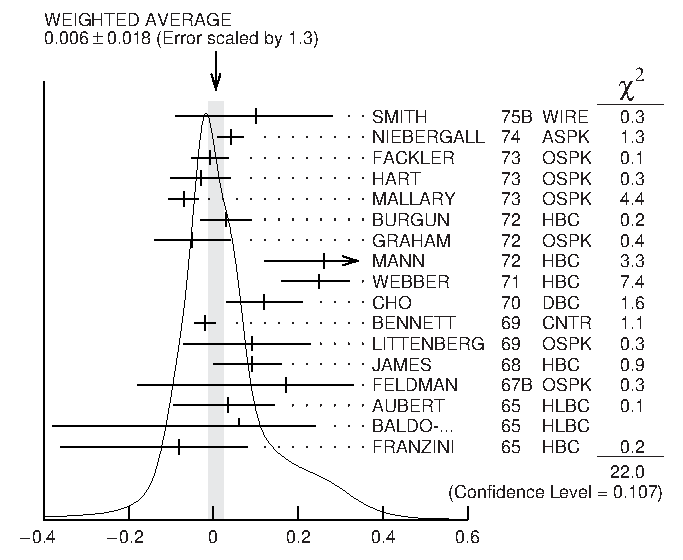
\includegraphics{filename} %multiple includegraphics may be used, 
	% with usual \hfill and \\ newline structures. 
\end{pdgxfigure}
\end{verbtex}

Figures placed in the \invt{figures} directory will be automaticallly found. 
Option keys may also be passed to individual \lstinline{\includegraphics} commands,  
as usual, if separate control is desired of multiple \lstinline{\includegraphics} in the same \invt{pdgxfigure} environment.
I.e. \lstinline!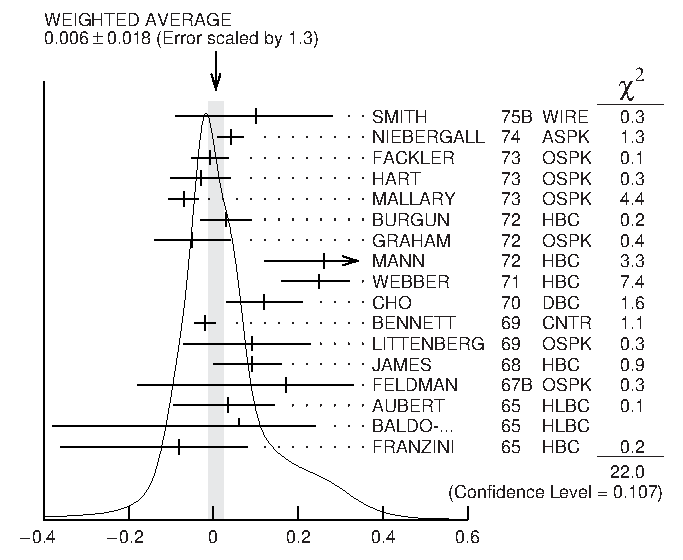
\includegraphics[<option keys>]{filename}!.

\Isubsection{Float scaling and width keys}
\label{sec:ginkeys}
As in the usual implementation of the \invt{graphicx} package, the \lstinline{\includegraphics} command takes optional standard keys \invt{width = ...}, \invt{scale = ...}.
which are used to control the width or scale of the bounding box. 
We use the same key structure to pass options to the \invt{pdgxfigure} environment, as well as to the \invt{pdgxtable} environment (see Sec.~\ref{sec:tables}).

The version specific keys \lstinline!<version>width! and \lstinline!<version>scale! have been added, 
that implement width or scaling choices only in the specific \invt{<version>}.
One may use these keys in concert with the usual \invt{width} and \invt{scale} keys, with the caveat that the order of keys matters: 
Keys are read left to right, and rightwards keys typically override leftwards ones. 
For example, passing the option keys (to either \invt{pdgxfigure} or \invt{pdgxtable}, or \lstinline{\includegraphics})
\begin{verbtex}
	[width=0.8\linewidth, bookwidth=0.9\linewidth]
\end{verbtex}
implements the \invt{width} key setting except in the book version. 
The option \lstinline!bookwidth=0.9\linewidth! followed by
\lstinline!width=0.8\linewidth! would instead implement only the version-general \lstinline!width=0.8\linewidth! setting.

\textbf{Note:} Because of specialization of the \invt{graphicx} key structure in the PDG class,
to use a \invt{scale} or \invt{<version>scale} key in an \lstinline{\includegraphics} command or \invt{pdgxfigure} environment
one must first pass an option key \invt{width=!}. This is not required for  \invt{pdgxtable}.

An additional key \lstinline!<version>bbscale! scales the float bounding box.
For some overwide floats that are larger than the nominal page width---in particular, overwide tables, see Sec.~\ref{sec:tables}---simply 
rescaling down the float does not allow it to be properly aligned on the page.
This key can be increased above $1$ (the default), to provide a sufficiently large bounding box for the float, that may then be scaled down to size with correct alignment.

\Isubsection{Available keys for \invt{pdgxfigure}}
Following is a list of available optional keys for \invt{pdgxfigure}, and default settings if not invoked.
As usual, keys are evaluated left to right. 
The version-general \invt{width} key can be used (and will override any preceeding version-specfic width key).
\begin{itemize}
	\item \invt{place}: Takes any combination of \invt{h}, \invt{t}, \invt{b}, \invt{p} (with optional \invt{\!}) that specifies float placement. Default is \invt{\!ht}.
	\item \invt{wide}: Takes \invt{true} or \invt{false} to specify the figure as full page width in either single or two column mode. Default is \invt{false}.
	\item \invt{width} or \invt{<version>width}: Sets the global or version specific width of the figure bounding box, respectively. Default is 0.75 of the line width (or text width, for wide figures).
	\item \invt{scale} or \invt{<version>scale}: Scales the figure according to float value passed to the key. 
	The option \lstinline{width=!} must be passed to turn off default width behavior and enable scaling keys.
\end{itemize}

\Isubsection{Examples}
The following produces a default-style, shown in Figure~\ref{examples:fig:example}. 
We recommend including the file extension in the \lstinline{\includegraphics} argument, to assist our editorial staff in addressing any figure quality problems.
\begin{verbtex}
\begin{pdgxfigure}[place=t] 
	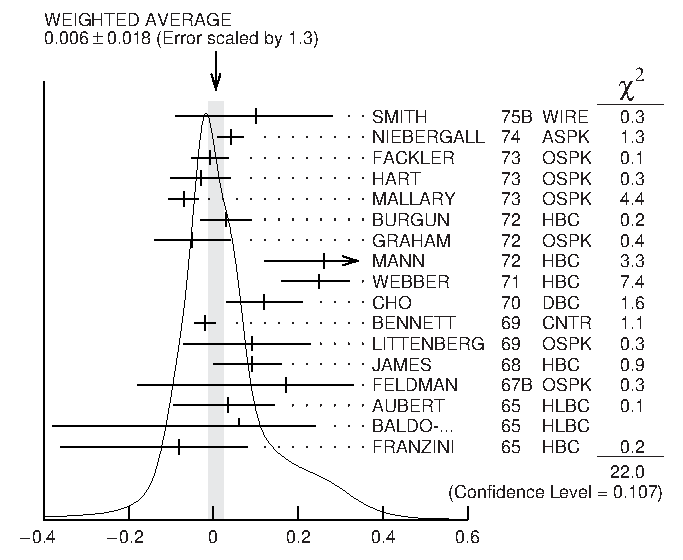
\includegraphics{filename.pdf}
	\caption{Example default figure}
	\label{examples:fig:example}
\end{pdgxfigure}
\end{verbtex}
\begin{pdgxfigure}[place=t]
	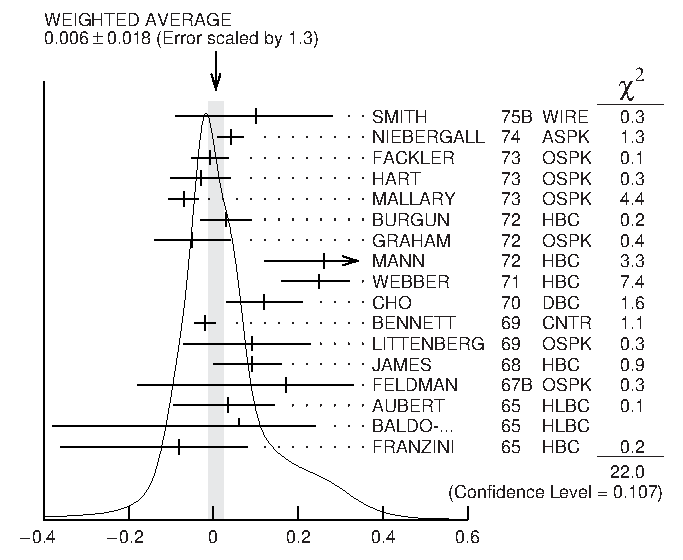
\includegraphics{filename.pdf}
	\caption{Example default figure}
	\label{examples:fig:example}
\end{pdgxfigure}

A double wide figure, shown in Fig.~\ref{examples:fig:example2}:
\begin{verbtex}
\begin{pdgxfigure}[wide=true,place=h, webwidth=0.45\linewidth, 
		bookwidth=0.9\linewidth] 
	%width key applies to all includegraphics instances
	%compiling in different versions will produce different widths
	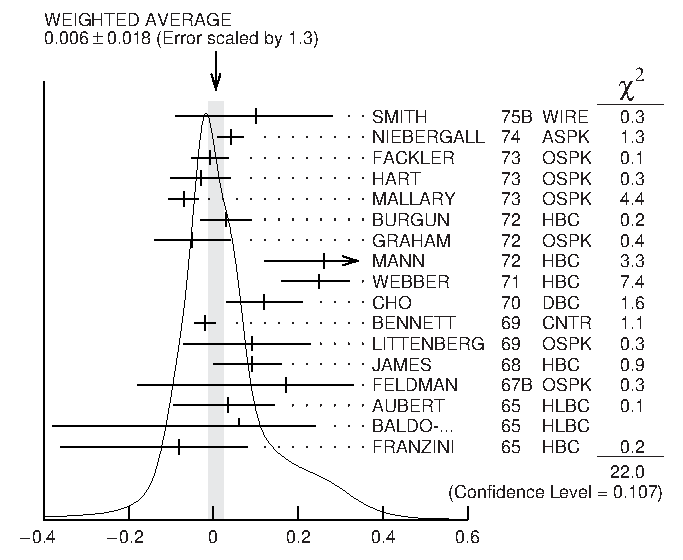
\includegraphics{filename.pdf}\hfill
	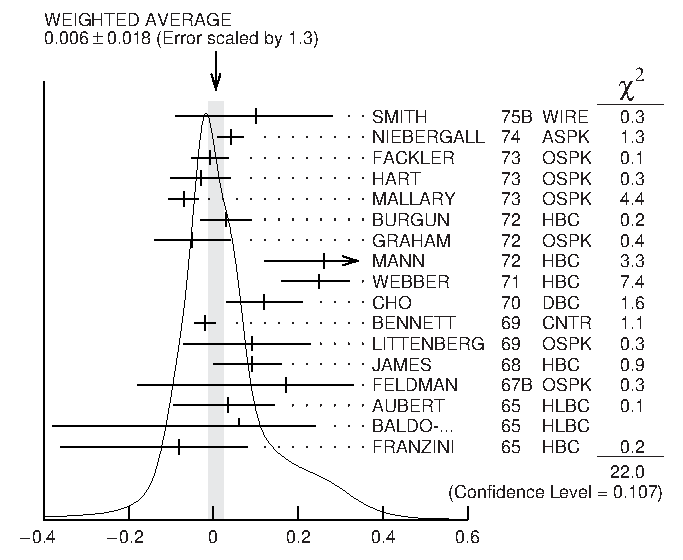
\includegraphics{filename.pdf}
	\caption{Example double wide figure, 
		with different book and web versions}
	\label{examples:fig:example2}
\end{pdgxfigure}
\end{verbtex}
\begin{pdgxfigure}[wide=true,place=h,width=0.45\textwidth] 
	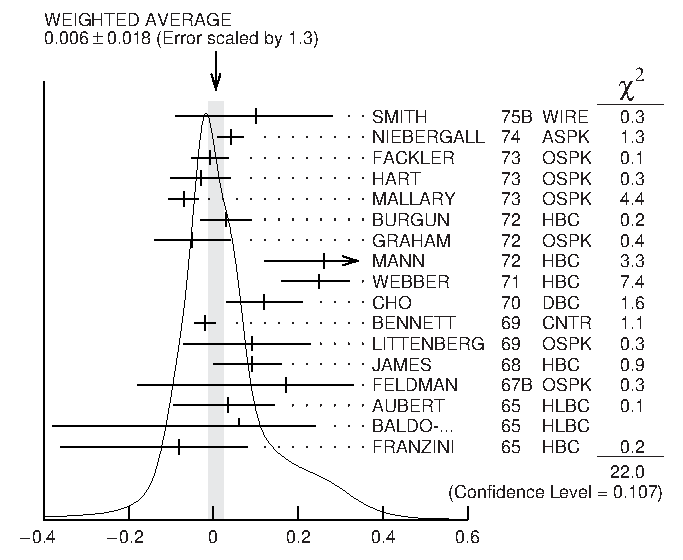
\includegraphics{filename.pdf}\hfill
	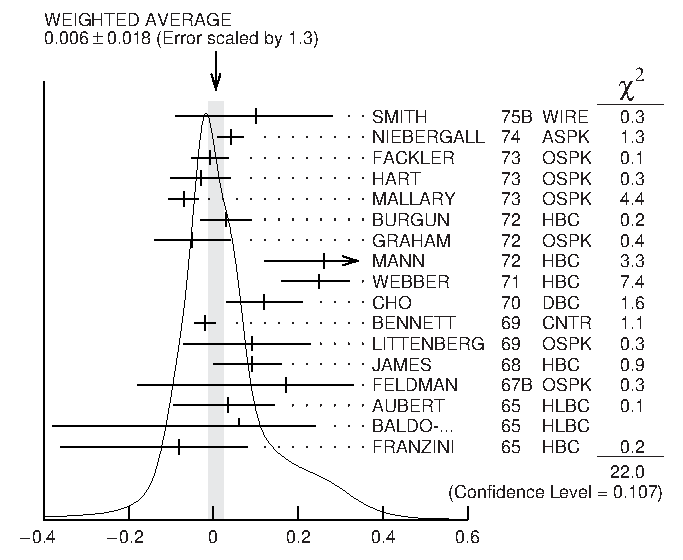
\includegraphics{filename.pdf}
	\caption{Example double wide figure, with different book and web versions}
	\label{examples:fig:example2}
\end{pdgxfigure}

A double wide figure with separate option and scaling keys, shown in Fig.~\ref{examples:fig:example3}:
\begin{verbtex}
\begin{pdgxfigure}[wide=true,place=h,width = 0.3\linewidth] 
	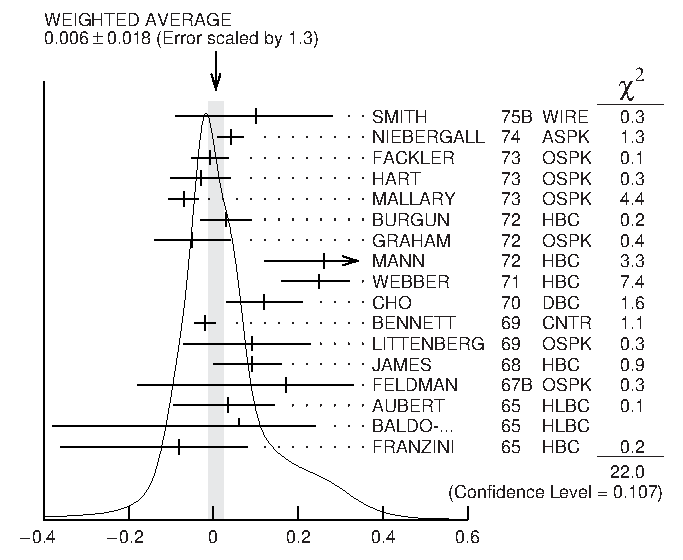
\includegraphics{filename.pdf}\hspace{1cm}
	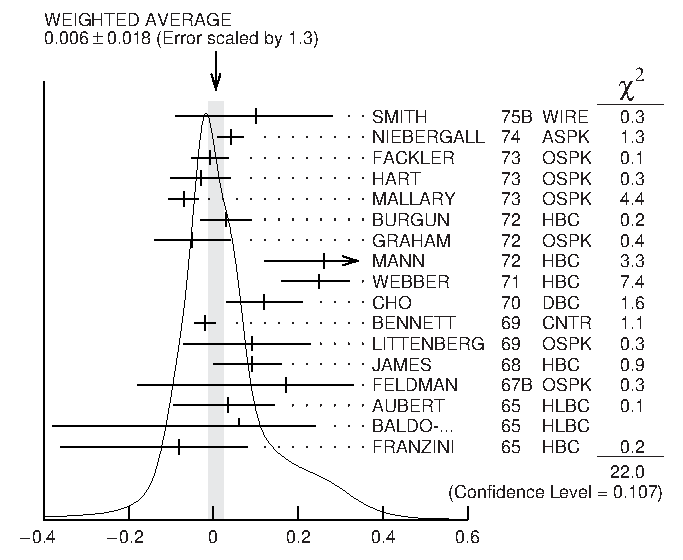
\includegraphics[width = !,scale =0.3,angle = 90]{filename}
	\caption{Example double figure, 
		with separate option and scaling keys, in both book and web versions}
	\label{examples:fig:example3}
\end{pdgxfigure}
\end{verbtex}
\begin{pdgxfigure}[wide=true,place=h,width = 0.3\linewidth] 
	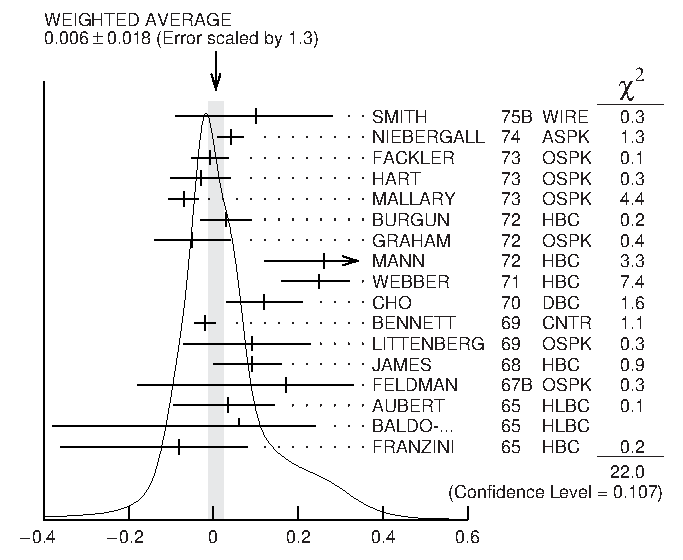
\includegraphics{filename.pdf}\hspace{1cm}
	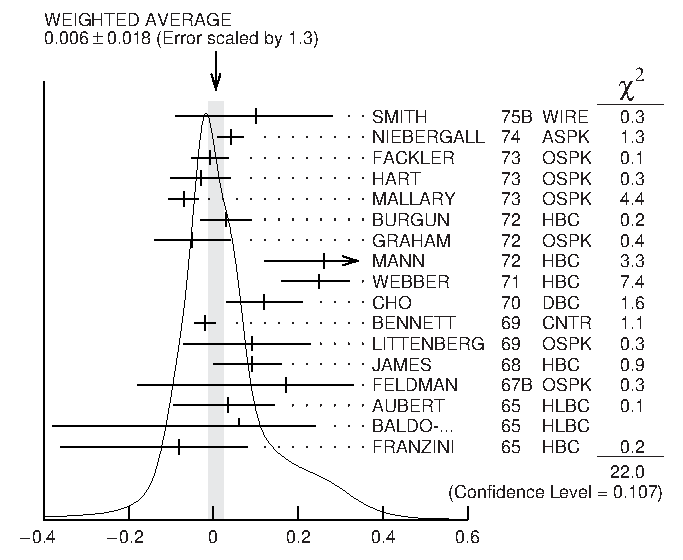
\includegraphics[width = !,scale =0.3,angle = 90]{filename}
	\caption{Example double wide figure, with separate option and scaling keys, in both book and web versions}
	\label{examples:fig:example3}
\end{pdgxfigure}

\Isubsection{\invt{pdgfigure} commands}
To add a figure, one may also use the \lstinline{\pdgfigure} or \lstinline{\pdgwidefigure} commands 
to typeset a single-column figure or double-column wide figure (for the book version), respectively. 
To include two images in one figure one may use \lstinline{\pdgdoublefigure}.
These commands are less powerful than \invt{pdgxfigure}, but automatically incorporate all PDG styles.

The macros \lstinline{\pdgfigure} and \lstinline{\pdgwidefigure} take the following arguments:
\begin{verbtex}
	\pdgfigure{<filename>}
	{<caption>}{<label>}{<placement options>}
	{<other option keys>}
\end{verbtex}
\vspace{-10pt}
while the macro \lstinline{\pdgdoublefigure} takes the following arguments:
\begin{verbtex}
	\pdgdoublefigure{<filename1>}{<filename2>}
	{<caption>}{<label>}{<placement options>}
	{<other option keys>}
\end{verbtex}
Some examples of the \invt{pdgfigure} commands are shown in Figs.~\ref{examples:fig:ideogram1}, \ref{examples:fig:ideogram2} and \ref{examples:fig:ideogram3}, respectively:
\begin{verbtex}
	\pdgfigure{filename.pdf}{Figure with caption and label}
	{examples:fig:ideogram1}{ht!}{}
	
	\pdgdoublefigure{filename.pdf}{filename.pdf}
	{Two figures, with caption and label, reduced in size}
	{examples:fig:ideogram2}{ht!}{width=0.3\textwidth}
	
	\pdgwidefigure{filename.pdf}{Wide figure}
	{examples:fig:ideogram3}{t}{}
\end{verbtex}
\FloatBarrier
\pdgfigure{filename.pdf}{Figure with caption and label}{examples:fig:ideogram1}{ht!}{}
\pdgdoublefigure{filename.pdf}{filename.pdf}{Two figures, with caption and label, reduced in size}{examples:fig:ideogram2}{ht!}{width=0.3\textwidth}
\pdgwidefigure{filename.pdf}{Wide figure}{examples:fig:ideogram3}{t}{}
\FloatBarrier

\Isection{Tables}
\label{sec:tables}
\Isubsection{ \invt{pdgxtable} and \invt{pdgxtabular}}
The PDG class provides multipurpose table and tabular environments, \invt{pdgxtable} and \invt{pdgxtabular}. 
These operate similarly to the standard \invt{table} and \invt{tabular} environments: \invt{(pdgx)table} creates a floating environment, 
while \invt{(pdgx)tabular} creates the actual tabulated display. 

The \lstinline!\caption! and \lstinline!\label! commands may be used as in the usual \invt{table} environment.
\textbf{Note: A table caption should be placed above the table.}
In addition, \invt{pdgxtable} takes a wide array of additional option keys that implement features and formatting of the prior PDG table commands/environments.  
These include keys that control placement, multicolumn spanning, version-specific widths and scaling (see Sec.~\ref{sec:ginkeys}), rotation, stretching, and caption widths.
The generic usage is
\begin{verbtex}
\begin{pdgxtable}[<option keys>]
	\caption{This is a PDG table}
	\label{tab:label}
	\begin{pdgxtabular}{<column settings>} % the usual c, l, r, | etc
		\pdgtableheader{...} %column header & separated entries go here
		%table & separated entries go here
	\end{pdgxtabular}
	%multiple pdgtabular environments are allowed
\end{pdgxtable}
\end{verbtex}

As for the usual \invt{table} environment, one may include multiple \invt{pdgxtabular}s in a single \invt{pdgxtable}.
While the \invt{pdgxtable} environment has default handling for caption widths in wide and regular tables, for both book and web versions, 
absolute control of the caption width can be implmented with a \lstinline{\captionsetup} command inside the \invt{pdgxtable} environment. 
For example \lstinline!\captionsetup{width=\linewidth}! gives a full width caption.

\Isubsection{Available keys for \invt{pdgxtable}}
Following is a list of available optional keys, and default settings if not invoked.
As usual, keys are evaluated left to right. 
While, the version-general \invt{width} key can be used (and will override any preceeding version-specfic width key), 
there is no version-general \invt{scale} key. 
Scaling of the tables is best done with the \invt{<version>scale} keys.

\begin{itemize}
	\item \invt{place}: Takes any combination of \invt{h}, \invt{t}, \invt{b}, \invt{p} (with optional \invt{\!}) that specifies float placement. Default is \invt{\!ht}.
	\item \invt{wide}: Takes \invt{true} or \invt{false} to specify the table as full page width in either single or two column mode. Default is \invt{false}.
	\item \invt{width} or \invt{<version>width}: Sets the version specific maximum width of the table bounding box. 
	Default is the maximum text width implied by the \invt{wide} key setting.
	Width settings exceeding this default are ineffective. Footnotes are scaled, but caption width is not affected.
	\item \invt{<version>scale}: Scales the table according to float value passed to the key. 
	For overwide tables, there is always a value $<1$ at which the table will be properly set to maximum page width.
	Footnotes are scaled, but caption width is not affected. Note the global \invt{scale} is disabled for \invt{pdgxtable}.
	\item \invt{<version>bbscale}: Scales the bounding box of the table. 
	For some overwide tables that are larger than the nominal page width, simply rescaling down the table does not allow the table to be properly aligned on the page.
	This key can be increased above $1$ (the default), to provide a sufficiently large bounding box for the table, that may then be scaled down to size with correct alignment.
	\item \invt{widecaptionscale}: For \invt{wide = true} tables, scales the caption width with respect to the maximum page width. Default is $0.75$.
	\item \invt{narrowcaptionscale}: For \invt{wide = false} or default tables, scales the caption width with respect to the maximum column width. Default is $0.9$.
	\item \invt{rotated}: Takes \invt{left} or \invt{right} to rotate the table, but not the caption, $90^\circ$ anticlockwise or clockwise, respectively. 
	The caption may be rotated independently, as needed with a \lstinline{\rotatebox}.
	\item \invt{sideways}: Takes \invt{true} or \invt{false} to rotate the table, including the caption, $90^\circ$ anticlockwise or clockwise, 
	according to whether the page number is even or odd.
	In a sideways table, other key width and scaling settings are still effective, but scale with respect to the page height. 
\end{itemize}


\Isubsection{Examples}
Some (simple) examples of \invt{pdgxtable} can be found in Table~\ref{examples:tab:styles} and Sec~\ref{sec:macros}.
For example, Tab.~\ref{examples:tab:styles} is typeset as
\begin{verbtex}
\begin{pdgxtable}[place=h,bookscale = 0.9,bookbbscale=2]
	\caption{Styles for the different typesetting versions}
	\label{examples:tab:styles}
	\begin{pdgxtabular}{ccccc}
		Version 		& Columns  & Font size 	& Helper Tags\footnote{
			Tags for each equation, table, figure, and bibliography entry 
			are displayed in margin or interspaced} & Line numbers\\
		\hline
		draft	& 1		   & 11pt		& Yes & Yes \\
		...
	\end{pdgxtabular}
\end{pdgxtable}
\end{verbtex}

Tables~\ref{examples:tab:commu} and~\ref{examples:tab:commp} are typeset as a two \invt{pdgxtabular}s in a single \invt{pdgxtable}, via
\begin{verbtex}
\begin{pdgxtable}[wide=true, place=!ht, webscale = 0.8]
	\caption{Common units}
	\label{examples:tab:commu}
	\begin{pdgxtabular}{lr | lr | lr}
		\showsymbol{\TeV} &  \showsymbol{\syin} & \showsymbol{\barn}   \\
		...
	\end{pdgxtabular}
	\caption{Common particles}
	\label{examples:tab:commp}
	\begin{pdgxtabular}{lr | lr | lr}
   		\showsymbol{\pp} &  \showsymbol{\ee} & \showsymbol{\pizero}   \\
  		...
	\end{pdgxtabular}
\end{pdgxtable}
\end{verbtex}

\Isubsection{Common problems and recommendations}
The \invt{pdgxtabular} environment is capable of handling the usual \lstinline{\multicolumn} and \lstinline{\multirow} objects, 
that allow for more complicated tables with cells spanning multiple rows and/or columns. 
We recommend avoiding use of \lstinline{\multispan}. 
For multiline cells, the \lstinline{\makecell} command from the \invt{makecell} package is recommended.

\Isection{Labels and referencing}
\label{sec:labels}

\Isubsection{Style guide}
As usual, the \lstinline{\label} and \lstinline{\ref} commands (and their derivatives) may be used to reference equations, tables, figures, and so on. 
To permit easy cross-referencing throughout the entire review, we request that you use the following labelling convention: \invt{BASENAME:type:name}
with \invt{type} corresponding to one of the following options
\begin{itemize}
\item {\tt fig} for figures
\item {\tt eq } for equation
\item {\tt tab} for tables
\item {\tt sec} for section, subsection etc..
\item {\tt foot} for footnotes.
\end{itemize}

\Isubsection{Missing references}

In default LaTeX, missing references are typically typeset as ``\textbf{??}''. 
To improve the typesetting experience, the \lstinline{\ref} command has been modified in the PDG class so that missing reference keys are printed out explicitly: 
For instance, a \lstinline!\ref{eqn:name}! that references a missing label called \invt{eqn:name}, will display as \ref{eqn:name}.
Similarly, the \lstinline{\cite} command will explicitly print out missing citation references. E.g. 
a \lstinline!\cite{name:2021ab}! that references a missing label called \invt{name:2021ab}, will display as \cite{name:2021ab}

\Isubsection{Cross-review referencing}
It is occasionally necessary or useful to reference (sub)sections, equations, figures, tables and so on belonging to other reviews or other reviews themselves. 
\textbf{Note:} Please use the \lstinline{\crossref} command for cross-review referencing.

Implementing a cross-reference to another review requires knowledge of its  \invt{BASENAME}:  
You must use the \invt{BASENAME} associated with the target review, not the \invt{BASENAME} of the review you're currently working on. 
To identify the  \invt{BASENAME} of another review, login into the \href{https://pdgworkspace.lbl.gov/Reviews.action}{PDG Workspace} (click to be redirected). 
Under \emph{Reviews} select from the drop-down menu \emph{All reviews}. 
Click on the title of the review you are interested in, and then select the \emph{Technical details} tab. 
The \invt{BASENAME} is the first entry.


If the full \invt{BASENAME:type:name} reference is known, you may include it with the usage \\
\lstinline!\crossref{BASENAME:type:name}!. 
This will typeset in your document as ``\crossref{BASENAME:type:name}'', because your local auxiliary files do not have the reference information of the other review.
PDG editorial staff will implement the cross-reference properly, when your review is prepared for production.

If the \invt{BASENAME:type:name} reference is not known, or the authors of the other review did not label the obect that you wish to reference, 
you may instead provide any descriptive argument to \lstinline{\crossref}. 
For example, \lstinline!\crossref{Equation 34.1.10}!.  
PDG editorial staff will implement the cross-reference properly, when your review and the other review are prepared for production.

\Isubsection{Booklet labeling and referencing}
If your review has a booklet version, it needs to be prepared at the same time as you prepare your full review.
The content to be displayed in the booklet needs to be included in \invt{BASENAME-booklet.tex}. 

The numerical tags for equations, tables, and figures in the booklet version of a review should match the tags in the full version. 
This can be achieved automatically in the booklet version by using a \lstinline!\tag{\ref{BASENAME:type:name}}! construction instead of \lstinline{\label}
to refer to the reference in the full version.
For example, if the full version has a labelled equation
\begin{verbtex}
\begin{equation}
	\label{BASENAME:eq:name}
	...
\end{equation}
\end{verbtex}
then including in \invt{BASENAME-booklet.tex}
\begin{verbtex}
\begin{equation}
	\tag{\ref{BASENAME:eq:name}}
	...
\end{equation}
\end{verbtex}
will automatically label the equation correctly. 
To achieve the same result for figures and tables, one may place in the booklet version
\begin{verbtex}
	\renewcommand{\thetable}{\ref{BASENAME:type:name}}
	\renewcommand{\thefigure}{\ref{BASENAME:type:name}}
\end{verbtex}
before each table or figure environment, respectively. 


\Isection{Index entries}
\label{sec:index}

Review authors should think about any keywords that should be included into the index of the Review of Particle Physics. PDG uses the standard \LaTeX\  \invt{makeidx} package. Thus an entry ``sample text'' can be added to the index by placing
\begin{verbtex}
\index{sample text}
\end{verbtex}
at the appropriate place in the source file. Formatting of entries with Greek letters or math symbols as well as subentries are also supported. For example
\begin{verbtex}
\index{sigma@$\$$\sigma$\$$} 
\end{verbtex}
creates an index entry $\sigma$ in the proper alphabetical order, while
\begin{verbtex}
\index{Searches!Axion searches} 
\end{verbtex}
produces a subentry ``Axion searches'' under the ``Searches'' index entry.

All index entries defined in a given review will be shown on the last page when the draft version is made. PDG staff will standardize all index entries during the final processing of all reviews. Therefore what matters is not the final formatting of index entries but that all relevant entries are added in the correct place.


\Isection{Bibliography}
\label{sec:cites}

Citations are handled using BibTeX. To add a citation to your review:
\begin{itemize}
\item Look up the reference in INSPIRE and download its BibTeX entry (see bottom of the \emph{Information} tab for the article, under \emph{Export}).
\item Add the BibTeX entry to the \invt{BASENAME.bib} file. Note the article tag assigned by INSPIRE: You can see it in the first line of the BibTeX entry, after \lstinline!@article{!.
\item Cite the reference with \lstinline{\cite}, using the article tag assigned by INSPIRE.
\end{itemize}

For example, to add a reference to the Review of Particle Physics (2018) 
add the following code to \invt{BASENAME.bib}:
\begin{verbtex}
@article{Tanabashi:2018oca,
      author         = "Tanabashi, M. and others",
      title          = "{Review of Particle Physics}",
      collaboration  = "Particle Data Group",
      journal        = "Phys. Rev.",
      volume         = "D98",
      year           = "2018",
      number         = "3",
      pages          = "030001",
      doi            = "10.1103/PhysRevD.98.030001",
      SLACcitation   = "%%CITATION = PHRVA,D98,030001;%%"
 }
\end{verbtex}
and then one may add a reference to it in \invt{BASENAME-main.tex} via \lstinline!\cite{Tanabashi:2018oca}!.

If a BibTeX entry downloaded from INSPIRE does not render correctly, 
you should first make sure you have the latest PDG style files, by running \invt{svn update} (after committing any edits you have made).
If this doesn't fix the issue please contact \invt{latexsupport@pdg.lbl.gov} for advice.  
If it appears, however, to be simply a mistake in INSPIRE's entry, 
rename the label to the form \invt{BASENAME:<INSPIRE label>} and then edit the entry as needed.
\textbf{Please do not edit entries downloaded from INSPIRE without changing the label.}
Changing the label will permit PDG editorial staff to easily identify and track edited citations, as well as notify INSPIRE of required corrections.
In case the reference does not appear in INSPIRE at all, please also use the convention for the label: \invt{BASENAME:name}.

Multiple references can be added to a single set of brackets with \lstinline!\cite{cite-key-1,cite-key-2,...}!.
One may group multiple references into the same numerical citation tag, using a \invt{*} prefix on subsequent citation keys: For example \lstinline!\cite{cite-key-1,*cite-key-2,*cite-key-3}!.
If a paper citation key is preceded by the asterisk, it can't be cited separately later, and doing so will result in a compilation error.
We recommend citing papers individually, without using the asterisk to group them.


\Isection{Footnotes}
Footnote styles are standardized throughout the review. In (rare) cases that the style needs to be changed, this is achieved via \lstinline!\setfootnotestyle{<style>}!,
where \invt{<style>} can be \lstinline{\fnsymbol} or \lstinline{\alph}, \lstinline{\Alph}, \lstinline{\arabic}, \lstinline{\roman}, \lstinline{\Roman} etc.

Sometimes the \LaTeX \ engine miscalculates the amount of space required for a footnote, resulting in overprinting of the footer.
One can help the engine obtain a better estimate by adjusting the effective page size. 
This can be done by placing \lstinline!\enlargethispage{-2\baselineskip}! somewhere just before the \lstinline{\footnote}; the \invt{-2} may be changed to any number. 

\Isection{Miscellaneous control commands}

\Isubsection{Unbalanced last page}
In the book version, the columns of the final page are automatically balanced. 
If this behavior is undesired, it may be altered by invoking \lstinline!\balancedlastpagefalse!.
The invocation may be added anywhere in the document.

\Isubsection{Blank last page}
In the book version, a blank final page may be added via \lstinline!\blankendpagetrue!.
The invocation may be added anywhere in the document.

\Isubsection{Book-only reviews}
Certain reviews are typeset for the web using the book version formatting. 
This is enforced automatically within the PDG system by \lstinline!\def\iswebbook{1}! before the \lstinline{\documentclass} invocation. 
The draft version, however, for such reviews are typeset in the usual draft/web format.

\clearpage
\Isection{PDG Macros}
\label{sec:macros}

\begin{pdgxtable}[wide=true, place=!ht, webscale = 0.8]
	\vspace{-10pt}
	\caption{Common units}
	\label{examples:tab:commu}
	\begin{pdgxtabular}{lr | lr | lr}
		\showsymbol{\TeV     } &  \showsymbol{\syin} & \showsymbol{\barn     }   \\
		\showsymbol{\MeV     } &  \showsymbol{\inch} & \showsymbol{\mbarn    }   \\
		\showsymbol{\keV     } &  \showsymbol{\ft  } & \showsymbol{\microbarn}   \\
		\showsymbol{\eV      } &  \showsymbol{\km  } & \showsymbol{\nb       }   \\
		\showsymbol{\GeVc    } &  \showsymbol{\m   } & \showsymbol{\pb       }   \\
		\showsymbol{\GeVcSq  } &  \showsymbol{\cm  } & \showsymbol{\fb       }   \\
		\showsymbol{\GeVcc   } &  \showsymbol{\mm  } & \showsymbol{\invnb    }   \\
		\showsymbol{\GeVccSq } &  \showsymbol{\mum } & \showsymbol{\invpb    }   \\
		\showsymbol{\MeVc    } &  \showsymbol{\nm  } & \showsymbol{\invfb    }   \\
		\showsymbol{\MeVcc   } &  \showsymbol{\fm  } & \showsymbol{\invab    }   \\
		\showsymbol{\invps   } &  \showsymbol{\nm  } & \showsymbol{\lum      }   \\
			&&  \showsymbol{\ma  } &&  \\
		\showsymbol{\degr    }  &  \showsymbol{\cma } && \\
			&&  \showsymbol{\mma } &&   \\
			&&  \showsymbol{\muma} &&   \\
	\end{pdgxtabular}
	\vspace{10pt}
	\caption{Common particles}
	\label{examples:tab:commp}
	\vspace{-10pt}
	\begin{pdgxtabular}{lr | lr | lr}
   \showsymbol{\pp         } &  \showsymbol{\ee           } & \showsymbol{\pizero   }   \\
   \showsymbol{\pbar       } &  \showsymbol{\epm          } & \showsymbol{\piplus   }   \\
   \showsymbol{\ppbar      } &  \showsymbol{\epem         } & \showsymbol{\piminus  }   \\
   \showsymbol{\tbar       } &  \showsymbol{\en           } & \showsymbol{\pipm     }   \\
   \showsymbol{\ttbar      } &  \showsymbol{\ep           } & \showsymbol{\pimp     }   \\
   \showsymbol{\bbar       } &  \showsymbol{\mumu         } & \showsymbol{\etaprime }   \\
   \showsymbol{\bbbar      } &  \showsymbol{\mun          } & \showsymbol{\Kzero    }   \\
   \showsymbol{\cbar       } &  \showsymbol{\mup          } & \showsymbol{\Kzerobar }   \\
   \showsymbol{\ccbar      } &  \showsymbol{\tautau       } & \showsymbol{\kaon     }   \\
   \showsymbol{\sbar       } &  \showsymbol{\taup         } & \showsymbol{\Kplus    }   \\
   \showsymbol{\ssbar      } &  \showsymbol{\taum         } & \showsymbol{\Kminus   }   \\
   \showsymbol{\ubar       } &  \showsymbol{\lepton       } & \showsymbol{\KzeroL   }   \\
   \showsymbol{\uubar      } &  \showsymbol{\leptonm      } & \showsymbol{\Kzerol   }   \\
   \showsymbol{\dbar       } &  \showsymbol{\ellm         } & \showsymbol{\Klong    }   \\
   \showsymbol{\ddbar      } &  \showsymbol{\leptonp      } & \showsymbol{\KzeroS   }   \\
   \showsymbol{\fbar       } &  \showsymbol{\ellp         } & \showsymbol{\Kzeros   }   \\
   \showsymbol{\ffbar      } &  \showsymbol{\leptonlepton } & \showsymbol{\Kshort   }   \\
   \showsymbol{\qbar       } &  \showsymbol{\ellell       } & \showsymbol{\Kstar    }   \\
   \showsymbol{\qqbar      } &  \showsymbol{\enu          } & \showsymbol{\jpsi     }   \\
   \showsymbol{\nbar       } &  \showsymbol{\munu         } & \showsymbol{\Jpsi     }   \\
   \showsymbol{\nnbar      } &  \showsymbol{\taunu        } & \showsymbol{\psip     }   \\
   \showsymbol{\neutron    } &  \showsymbol{\lnu          } & \showsymbol{\chic     }   \\
   \showsymbol{\antineutron} &  \showsymbol{\nub          } & \showsymbol{\UoneS    }   \\
   \showsymbol{\deuteron   } &  \showsymbol{\nunub        } & \showsymbol{\chib     }   \\
   \showsymbol{\Zzero      } &  \showsymbol{\nue          } & \showsymbol{\Dstar    }   \\
   \showsymbol{\Zboson     } &  \showsymbol{\nueb         } & \showsymbol{\Bd       }   \\
   \showsymbol{\Wplus      } &  \showsymbol{\nuenueb      } & \showsymbol{\Bs       }   \\
   \showsymbol{\Wminus	   } &  \showsymbol{\num          } & \showsymbol{\Bu       }   \\
   \showsymbol{\Wboson	   } &  \showsymbol{\numb         } & \showsymbol{\Bc       }   \\ 
   \showsymbol{\Wpm   	   } &  \showsymbol{\numnumb      } & \showsymbol{\Lb       }   \\
   \showsymbol{\Wmp        } &  \showsymbol{\nut          } & \showsymbol{\Bstar    }   \\
   \showsymbol{\Hzero } &  \showsymbol{\nutb         } & \showsymbol{\BoBo     }   \\
   \showsymbol{\Hboson}  &	\showsymbol{\nutnutb      } & \showsymbol{\BodBod   }    \\		    
   \showsymbol{            } &	\showsymbol{              } & \showsymbol{\BosBos   }    \\		    
   \showsymbol{            } &	\showsymbol{              } & \showsymbol{\LambdaStar}  \\
	\end{pdgxtabular}
\end{pdgxtable}

\begin{pdgxtable}[wide=true, place=h, webscale = 0.8]
	\caption{Hypothetical particles}
	\begin{pdgxtabular}{lr | lr | lr}
   \showsymbol{\Azero }      &  \showsymbol{\gravino   } & \showsymbol{\slepton   }   \\
   \showsymbol{\hzero }      &  \showsymbol{\Zprime    } & \showsymbol{\sleptonL  }   \\
   \showsymbol{\Hzero }      &  \showsymbol{\Zstar     } & \showsymbol{\sleptonR  }   \\
   \showsymbol{\Hplus }  	  &  \showsymbol{\squark    } & \showsymbol{\sel       }   \\
   \showsymbol{\Hminus}       &  \showsymbol{\squarkL   } & \showsymbol{\selL      }   \\
   \showsymbol{\Hpm   }   	&  \showsymbol{\squarkR   } & \showsymbol{\selR      }   \\
   \showsymbol{\Hmp   }       &  \showsymbol{\gluino    } & \showsymbol{\smu       }   \\
   \showsymbol{\ggino }     &  \showsymbol{\stop      } & \showsymbol{\smuL      }   \\
   \showsymbol{\chinop}      &  \showsymbol{\stopone   } & \showsymbol{\smuR      }   \\
   \showsymbol{\chinom}      &  \showsymbol{\stoptwo   } & \showsymbol{\stau      }   \\
   \showsymbol{\chinopm}      &  \showsymbol{\stopL     } & \showsymbol{\stauL     }   \\
   \showsymbol{\chinomp}     &  \showsymbol{\stopR     } & \showsymbol{\stauR     }   \\
   \showsymbol{\chinoonep}     &  \showsymbol{\sbottom   } & \showsymbol{\stauone   }   \\
   \showsymbol{\chinoonem}   &  \showsymbol{\sbottomone} & \showsymbol{\stautwo   }   \\
   \showsymbol{\chinoonepm}   &  \showsymbol{\sbottomtwo} & \showsymbol{\snu       }   \\
   \showsymbol{\chinotwop}  &  \showsymbol{\sbottomL  } & \showsymbol{           }   \\
   \showsymbol{\chinotwom}   &  \showsymbol{\sbottomR  } & \showsymbol{           }   \\
   \showsymbol{\chinotwopm}   &  \showsymbol{           } & \showsymbol{           }   \\
   \showsymbol{\nino}  &  \showsymbol{           } & \showsymbol{           }   \\
   \showsymbol{\ninoone}        &  \showsymbol{           } & \showsymbol{           }   \\
   \showsymbol{\ninotwo}     &  \showsymbol{           } & \showsymbol{           }   \\
   \showsymbol{\ninothree}     &  \showsymbol{           } & \showsymbol{           }   \\
   \showsymbol{\ninofour}   &  \showsymbol{           } & \showsymbol{           }   \\
	\end{pdgxtabular}
\vspace*{10pt}
	\caption{Useful symbols for proton-proton physics}
\vspace*{-10pt}	
	\begin{pdgxtabular}{lr | lr }
   \showsymbol{\pT  }      &  \showsymbol{\rts }   \\
   \showsymbol{\pt  }      &  \showsymbol{\sqs } \\
   \showsymbol{\ET  }      &  \showsymbol{\mh}  \\
   \showsymbol{\eT  }      &  \showsymbol{\mW}  \\
   \showsymbol{\et  }      & \showsymbol{\mZ}   \\
   \showsymbol{\HT  }      & \showsymbol{\mH}   \\
   \showsymbol{\pTsq}      &&   \\
   \showsymbol{\MET }      &&   \\
   \showsymbol{\met }      &&   \\
   \showsymbol{\Ecm }      &&   \\
	\end{pdgxtabular}
\vspace*{10pt}
	\caption{Monte Carlo Generators}
\vspace*{-10pt}		
	\begin{pdgxtabular}{lr | lr | lr}	
   \showsymbol{\ACERMC    }      &  \showsymbol{\MCatNLO   } & \showsymbol{\Comphep    }   \\
   \showsymbol{\ALPGEN    }      &  \showsymbol{\AMCatNLO  } & \showsymbol{\Prospino   }   \\
   \showsymbol{\GEANT     }      &  \showsymbol{\MCFM      } & \showsymbol{\LO         }   \\
   \showsymbol{\Herwigpp  }      &  \showsymbol{\METOP     } & \showsymbol{\NLO        }   \\
   \showsymbol{\HERWIGpp  }      &  \showsymbol{\POWHEG    } & \showsymbol{\NLL        }   \\
   \showsymbol{\Herwig    }      &  \showsymbol{\POWHEGBOX } & \showsymbol{\NNLO       }   \\
   \showsymbol{\HERWIG    }      &  \showsymbol{\POWPYTHIA } & \showsymbol{\muF        }   \\
   \showsymbol{\JIMMY     }      &  \showsymbol{\PROTOS    } & \showsymbol{\muR        }   \\
   \showsymbol{\MADSPIN   }      &  \showsymbol{\PYTHIA    } & \showsymbol{            }   \\
   \showsymbol{\MADGRAPH  }      &  \showsymbol{\SHERPA    } & \showsymbol{            }   \\
   \showsymbol{\MGMCatNLO }      &  \showsymbol{           } & \showsymbol{            }   \\
	\end{pdgxtabular}
\end{pdgxtable}

\Isection{Tables: Legacy commands}

Though no longer recommended, legacy \lstinline{\pdgtable} or \lstinline{\pdgwidetable} commands 
to typeset a single-column table or double-column wide table (for the book version), respectively.
The \lstinline{\pdgtableheader} macro may be used in the first line of the table to automatically typeset a header.

The macros \lstinline{\pdgtable} and \lstinline{\pdgwidetable} take the following arguments:
\begin{verbtex}
	\pdgtable{<column styles>}
	{<caption>}{<label>}{<option keys>}
\end{verbtex}
Some examples usages of these commands follow, in Tables~\ref{examples:tab:table1}, \ref{examples:tab:table2} and~\ref{examples:tab:table3} below.
\begin{verbtex}
\begin{pdgtable}{c c c} 
	{Table}{examples:tab:table1}{h!}
	\pdgtableheader{ Column 1 & Column 2 & Column 3}
	row1  & 1  & 2\\
	row2  & 1  & 2\\
	row3  & 1  & 2\\
\end{pdgtable}
\end{verbtex}   
\begin{verbtex}
\begin{pdgtable}{|c | c | c | c|} 
	{Multicolumn table}{examples:tab:table2}{h!}
	\pdgtableheader{ \multicolumn{2}{c}{Column 1} & 
	\multicolumn{2}{c}{Column 2}}
	\pdgtableheader{ A & B& C & D }
	row1  & 1 & 2 &3 \\
	row2  & 1 & 2 &3 \\
\end{pdgtable}
\end{verbtex}  
\begin{verbtex}
\begin{pdgtable}{c l}
	{Table with footnotes}{examples:tab:table3}{}
	One value & another\footnote{This is something to notice
	\label{kmmix:foot:one}}\\
	Two values\footref{kmmix:foot:one} & another \\
\end{pdgtable}
\end{verbtex} 
 
\FloatBarrier 
\begin{pdgtable}{c c c} 
{Table}{examples:tab:table1}{h!}
\pdgtableheader{ Column 1 & Column 2 & Column 3}
row1  & 1  & 2\\
row2  & 1  & 2\\
row3  & 1  & 2\\
\end{pdgtable}
\begin{pdgtable}{|c | c | c | c|} 
{Multicolumn table}{examples:tab:table2}{h!}
\pdgtableheader{ \multicolumn{2}{|c|}{Column 1} & 
\multicolumn{2}{|c|}{Column 2}}
\pdgtableheader{ A & B& C & D }
row1  & 1 & 2 &3 \\
row2  & 1 & 2 &3 \\
\end{pdgtable}
\begin{pdgtable}{c l}
{Table with footnotes}{examples:tab:table3}{}
One value & another\footnote{This is something to notice\label{kmmix:foot:one}}\\
Two values\footref{kmmix:foot:one} & another \\
\end{pdgtable}
! line that includes these instructions in the main source file of your review, \invt{ml-main.tex}.

This documentation focuses mostly on the specialized functionality of the PDG \LaTeX \ class: %There are many resources that provide more general guidance for typesetting in \LaTeX.
For further support, or any \LaTeX-related questions, we invite authors to contact
\vspace{-0.2cm}
\begin{center}
\scalebox{1.5}{
	\invt{latexsupport@pdg.lbl.gov}
}
\end{center}

\Isubsection{File structure}
The source files for a PDG review are kept in separate directories within a SVN repository. 
Some files in each directory are auto-generated, while others are designed to be edited by review authors. 
\textbf{Do not edit auto-generated files, as any edits to these files will be overwritten periodically.}

Each review is assigned a unique name ("basename") that is used to label the relevant review files and will be referred to as \invt{BASENAME} in the following. For example, the QCD review is assigned basename \invt{qcd}. Therefore \invt{BASENAME-main.tex} in this documentation refers to file \invt{qcd-main.tex} for the QCD review.

Your review is assigned basename \invt{ml}.

The basename is further used to label cross-references to the review (see Sec.~\ref{sec:labels}) and specialized citations (see Sec.~\ref{sec:cites}). 
The file structure of a typical review is as follows:
\begin{itemize}
\item \invt{BASENAME-main.tex} --- contains the text of your review. 
\item \invt{BASENAME-booklet.tex} --- contains the text of the booklet version of your review (if there is one)
\item \invt{BASENAME-preamble.tex} --- contains review-specific definitions or inclusion of packages, that need to go into the document's preamble
\item \invt{BASENAME.bib} --- BibTeX bibliography entries (see Sec~\ref{sec:cites})
\item \invt{/figures} --- directory containing all figures
\item Auxiliary files (\invt{.aux}, \invt{.out}, \invt{.log}) --- these are generated by the \LaTeX compiler
\item Other \invt{.tex} files --- may be added and included in \invt{BASENAME-main.tex} or \invt{BASENAME-booklet.tex} with the \lstinline{\input} command.
\item \textbf{[auto-generated]} \invt{BASENAME.tex} --- compilation file for the review
\item \textbf{[auto-generated]} \invt{Makefile} --- Makefile to compile the review automatically (see Sec.~\ref{sec:make})
\item \textbf{[auto-generated]} \invt{pdg.cls} --- PDG \LaTeX \ class file
\item \textbf{[auto-generated]} \invt{pdg.bst} --- BibTeX PDG style file
\item \textbf{[auto-generated]} \invt{pdg-xr-hyper.sty} --- helper BibTeX style file
\item \textbf{[auto-generated]} \invt{pdgdefs.tex} --- PDG standard symbols and macros
\item \textbf{[auto-generated]} \invt{examples.tex} --- This file
\end{itemize}

\begin{center}
~\\
%!%\vspace{-12pt}
%!%In your review, the basename is ml.
\end{center}
To identify the  \invt{BASENAME} of yours or another review, you may also login into the 
\href{https://pdgworkspace.lbl.gov/Reviews.action}{PDG Workspace} (click to be redirected). 
Under \emph{Reviews} select from the drop-down menu \emph{All reviews}. 
Click on the title of the review you are interested in, and then select the \emph{Technical details} tab. 
The \invt{BASENAME} is the first entry.

\Isubsection{Multiversion typesetting}
The PDG \LaTeX \ class has functionality to typeset in four different versions or styles: draft, web, book and booklet. 
(The draft and web versions are referred to below jointly as `web', since they are broadly similar). 
See Table~\ref{examples:tab:styles} for a broad summary.

\begin{pdgxtable}[place=h,bookscale = 0.9,bookbbscale=2]
	\caption{Styles for the different typesetting versions}
	\label{examples:tab:styles}
	\begin{pdgxtabular}{ccccc}
		Version 		& Columns  & Font size 	& Helper Tags\footnote{
			Tags for each equation, table, figure, and bibliography entry are displayed in margin or interspaced} & Line numbers\\
		\hline
		\invt{draft} 	& 1		   & 11pt		& Yes & Yes \\
		\invt{web} 		& 1		   & 11pt		& No  & No\\
		\invt{book} 	& 2		   & 8pt		& No  & No\\
		\invt{booklet} 	& 1		   & 8pt		& No & No \\
	\end{pdgxtabular}
\end{pdgxtable}

Specialized macros may also have version-specific implementations. 
These follow the naming convention \invt{<version><macroname>}, where \invt{<version>} may take values of \invt{book}, \invt{booklet} and \invt{web}.
See for example, Sec.~\ref{sec:align}.
Specialized option keys follow the same convention. See e.g. Sec.~\ref{sec:ginkeys}.


\Isubsection{Makefile}
\label{sec:make}
We recommend to compile the review using \invt{make} on the command line. The usage is as follows:
\begin{itemize}
	\item \invt{make} --- compiles in draft mode.
	\item \invt{make  <version>} --- compiles in \invt{<version>} mode. For example \invt{make web}.
	\item \invt{make bib} --- compiles only the BibTeX files.
	\item \invt{make clean} --- cleans out all auxiliary files.
	\item \invt{make cleanall} --- cleans out the compiled pdf and all auxiliary files.
	\item \invt{make prod} --- cleans all auxiliary files, then compiles the web version.
	\item {\footnotesize{\texttt{make crossref}}} --- compiles required cross-referencing files (advanced: requires checkout of the other reviews to be cross-referenced).
\end{itemize}



\Isection{Style guides}
\Isubsection{Particle symbols}
Particle symbols are italic (or slanted) characters: \en, \pbar, \Lb, \pizero, \Klong, \Dstar. 
Charge is indicated by a superscript: $B^{-}$, $\Delta^{++}$. 
Charge is not normally indicated for $p$, $n$, or the quarks, and is optional for neutral isosinglets: $\eta$ or $\eta^{0}$. 
Antiparticles and particles are distinguished by charge for
charged leptons and mesons: $\tau^{+}$, $\kaon^{-}$ 
Otherwise, distinct antiparticles are indicated by a bar (overline): $\nbar_{\mu}$, \tbar, \pbar, \Kzerobar.

\Isubsection{Macros and shortcuts}
The \invt{pdgdefs.tex} file implements a series of useful macros for particle symbols, units and other common notation. 
All definitions are terminated with  \lstinline!\string\xspace!, so you can simply write ``\lstinline!\ttbar production!'' to typeset inline ``\ttbar production''.
The entire list of macros is provided in Sec.~\ref{sec:macros}.

Most Monte Carlo generators have a macro with a suffix 'V' that allows you to include the version. E.g. \lstinline!\PYTHIAV{8.1}! produces \PYTHIAV{8.1}.
In case you need to define other symbols, please add them to the \invt{BASENAME-preamble.tex} file.

\Isubsection{Column switching}

The web version is typeset as single column, singleside 11pt style, the book as 8pt double column, double sided.

In all versions of the review, switching between single and double column mode can be done \emph{in situ} with \lstinline{\onecolumn} or \lstinline{\twocolumn}
respectively. For example

\medskip
\ifrppbook
	\onecolumn
\else
	\twocolumn
\fi
{\footnotesize{Lorem ipsum dolor sit amet, consectetur adipiscing elit. Duis congue lectus at lectus tristique porta. Vivamus scelerisque porta massa, laoreet pulvinar dolor blandit vitae. Nam rhoncus id risus in tincidunt. Maecenas ultrices, arcu id gravida tempor, urna libero sodales nunc, quis dapibus ipsum quam eget est. Quisque eget convallis odio, at pellentesque quam. Mauris pretium eu metus ac imperdiet. Class aptent taciti sociosqu ad litora torquent per conubia nostra, per inceptos himenaeos. Nulla quis tincidunt libero. Aliquam posuere at quam quis posuere. Etiam turpis nulla, faucibus eget massa sagittis, porttitor sagittis elit. Proin a lorem eleifend, rhoncus orci quis, mattis metus. Donec sit amet lobortis lacus. Quisque magna augue, elementum nec ipsum non, feugiat ultricies urna. Sed tincidunt nisl vestibulum leo finibus, vitae sollicitudin sapien bibendum. Duis maximus ipsum nec urna lobortis, sed scelerisque nulla facilisis. Sed id finibus libero. }}
\ifrppbook
	\twocolumn
\else
	\onecolumn
\fi
\medskip

\Isection{Equations}
Equations may be typeset using the \invt{equation}, \invt{array}, \invt{multline}, and \invt{gather} etc environments provided by \invt{amsmath} package. 
We do not recommend using \invt{eqnarray}. As a trivial example
\begin{verbtex}
\begin{equation}
\label{BASENAME:eq:equation}
	N_{exp} = \sigma_{exp} \times \int L(t) dt
\end{equation}
\end{verbtex}
which produces
\begin{equation}
	N_{exp} = \sigma_{exp} \times \int L(t) dt
\end{equation}


To tag a set of equations with a common numbering and label, please use the \invt{subequation} environment, together with \invt{align}.
As an example:
\begin{verbtex}
\begin{subequations}
	\label{BASENAME:eq:equation1}
	\begin{align}
		A + B = C\\
		D= \frac{E}{F}  
	\end{align}
\end{subequations}
\end{verbtex}
which produces
\begin{subequations}
\begin{align}
	A + B = C\\
	D= \frac{E}{F}  
\end{align}
\end{subequations}


\Isubsection{Wide equations: \invt{pdgstrip}}
Some wide equations are not easily amenable to display in the PDG book double column format. 
Similar to the ReVTeX \invt{widetext} environment, the PDG style provides a \invt{pdgstrip} environment, that may wrap any other equation (or align, array etc) environment. 
The \invt{pdgstrip} environment is not a float, and will respect absolute placement in the typesetting stream. 
For example:
\begin{verbtex}
	\begin{pdgstrip}
		\begin{equation} % or any other display environment
		...

		\end{equation}
	\end{pdgstrip}
\end{verbtex}
In the web and booklet versions, this environment performs no operation on the wrapped environment. 
In the book version, the equation is preserved as a single `strip' across both columns, with column-wide rules to guide the reader's eye. 
The column-wide rules may be disabled -- e.g if the strip environment falls at the top or bottom of a page --  by passing the option \invt{plain} to the \invt{pdgstrip} environment. I.e. 
\lstinline!\begin{pdgstrip}[plain]!.

In principle, the pdgstrip envirornment may also wrap a floating environment such as a figure. 
In the book version, this will disable the ability of the figure to float, and fix it to a desired location.

\Isubsection{Alignment}
\label{sec:align}
Within \invt{align} environments or any other environment that uses the special \invt{&} and \invt{\\\\} (or \lstinline{\cr}) control characters for alignment, one may use
use version specific \lstinline!\bookalign!, \lstinline!\webalign!, \lstinline!\bookletalign! and \lstinline!\bookcr!, \lstinline!\webcr!, \lstinline!\bookletcr! macros.

The \lstinline!\<version>align! macros insert a `\invt{&}' control character only in the \invt{<version>} of the review. 
The \lstinline!\<version>cr! macro similarly inserts a carriage return `\invt{\\\\}' only in the \invt{<version>} of the review, 
but takes two additional arguments that are placed before and after the carriage return, respectively. For instance,
\lstinline!\bookcr{\nonumber}{[10pt]}! inserts \lstinline!\nonumber\\[10pt]!.  An example usage is
\begin{verbtex}
\begin{align}
	{\cal A}_f 
	\bookalign = \frac{\Gamma(\bar{B}^0(t) \to f) - \Gamma(B^0(t) \to f)}
		{\Gamma(\bar{B}^0(t) \to f) + \Gamma(B^0(t) \to f)} \bookcr{\,,\nonumber}{}
	\bookalign = S_f \sin(\Delta m_d\, t) - C_f \cos(\Delta m_d\, t) \,.
\end{align}
\end{verbtex}
This produces in the web version
\ifrppbook
\onecolumn
	\begin{align}
		{\cal A}_f  = \frac{ \Gamma(\bar{B}^0(t) \to f) - \Gamma(B^0(t) \to  f) }
			{ \Gamma(\bar{B}^0(t) \to f) + \Gamma(B^0(t) \to  f) } 
			= S_f \sin(\Delta m_d\, t) - C_f \cos(\Delta m_d\, t) \,,
	\end{align}
\twocolumn
\else
	\begin{align}
		{\cal A}_f 
		\bookalign = \frac{ \Gamma(\bar{B}^0(t) \to f) - \Gamma(B^0(t) \to  f) }
			{ \Gamma(\bar{B}^0(t) \to f) + \Gamma(B^0(t) \to  f) } \bookcr{\,,\nonumber}{}
		\bookalign = S_f \sin(\Delta m_d\, t) - C_f \cos(\Delta m_d\, t) \,,
	\end{align}
\fi	
and in the two column book version
\addtocounter{equation}{-1}
\ifrppweb
	\twocolumn
	\begin{align}
		{\cal A}_f 
		& = \frac{ \Gamma(\bar{B}^0(t) \to f) - \Gamma(B^0(t) \to  f) }
			{ \Gamma(\bar{B}^0(t) \to f) + \Gamma(B^0(t) \to  f) } \,,\nonumber\\
		& = S_f \sin(\Delta m_d\, t) - C_f \cos(\Delta m_d\, t) \,,
	\end{align}
	\onecolumn
\else
	\begin{align}
		{\cal A}_f 
		\bookalign = \frac{ \Gamma(\bar{B}^0(t) \to f) - \Gamma(B^0(t) \to  f) }
			{ \Gamma(\bar{B}^0(t) \to f) + \Gamma(B^0(t) \to  f) } \bookcr{\,,\nonumber}{}
		\bookalign = S_f \sin(\Delta m_d\, t) - C_f \cos(\Delta m_d\, t) \,,
	\end{align}
\fi

\Isection{Figures}

\Isubsection{Figure requirements}
Permitted figure formats (for pdflatex) are pdf, png and jpg, in order of preferred format. 
In addition, please note:
\begin{itemize}
	\item Submissions should be be provided with a minimum resolution of 150DPI. However, 300DPI or greater is preferred.
	\item Our preference for the submission color palette is CMYK, but RGB is acceptable.
	\item Visible line (stroke) weight must be no less than $0.5$px, preferably at least $1$px.
	\item Submissions should be provided with fonts embedded, if possible.
	\item In print, colors are often not as vibrant or saturated as they appear on screen. Therefore, overlapping areas of color should be high contrast for visual clarity: 
	e.g. do not place magenta over blue, or light blue over a light green.	
\end{itemize}
If you are unsure your figure is of sufficient resolution or quality, please contact \invt{latexsupport@pdg.lbl.gov} for advice.

Encapsulated postscript or postscript figures may also be used, but they require conversion to pdf. 
Depending on your \LaTeX \ engine settings, running \invt{pdflatex} may automatically convert eps or ps files. 
If not, the conversion can be done manually with various programs, such as ImageMagick, or \invt{epstopdf} and \invt{pstopdf}.

\textbf{Note:} Make sure that the figure file is added into the subdirectory \invt{figures}, and that it is commited to svn or provided with your text.

\Isubsection{\invt{pdgxfigure} environment}
The multipurpose figure environment \invt{pdgxfigure} is now available, as an alternative to the various \invt{pdgfigure} and related commands.
These operate similarly to the standard \invt{figure} environments: \invt{(pdgx)figure} creates a floating environment.

The \lstinline!\caption! and \lstinline!\label! commands may be used as in the usual \invt{figure} environment. 
\textbf{Note: A figure caption should be placed below the figure.}
In addition, \invt{pdgxfigure} takes an array of additional option keys that implement features and formatting of the prior PDG figure commands.
These include keys that control placement, multicolumn spanning, and version-specific widths. 
The generic usage is
\begin{verbtex}
\begin{pdgxfigure}[<option keys>]
	\caption{This is a PDG figure}
	\label{examples:fig:label}
	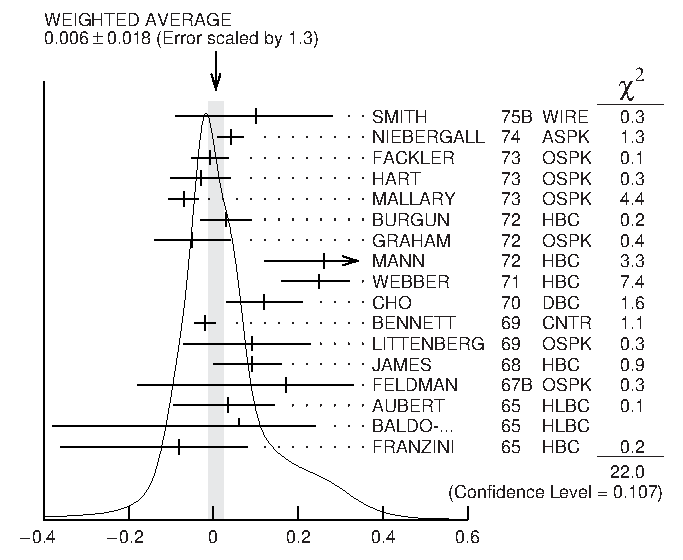
\includegraphics{filename} %multiple includegraphics may be used, 
	% with usual \hfill and \\ newline structures. 
\end{pdgxfigure}
\end{verbtex}

Figures placed in the \invt{figures} directory will be automaticallly found. 
Option keys may also be passed to individual \lstinline{\includegraphics} commands,  
as usual, if separate control is desired of multiple \lstinline{\includegraphics} in the same \invt{pdgxfigure} environment.
I.e. \lstinline!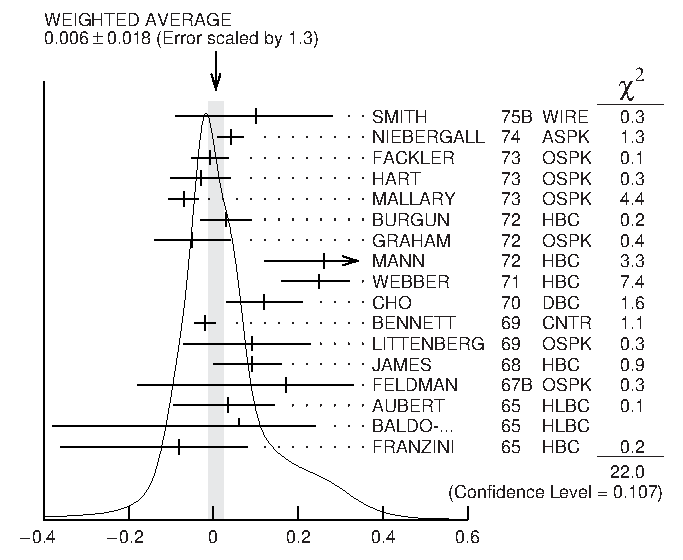
\includegraphics[<option keys>]{filename}!.

\Isubsection{Float scaling and width keys}
\label{sec:ginkeys}
As in the usual implementation of the \invt{graphicx} package, the \lstinline{\includegraphics} command takes optional standard keys \invt{width = ...}, \invt{scale = ...}.
which are used to control the width or scale of the bounding box. 
We use the same key structure to pass options to the \invt{pdgxfigure} environment, as well as to the \invt{pdgxtable} environment (see Sec.~\ref{sec:tables}).

The version specific keys \lstinline!<version>width! and \lstinline!<version>scale! have been added, 
that implement width or scaling choices only in the specific \invt{<version>}.
One may use these keys in concert with the usual \invt{width} and \invt{scale} keys, with the caveat that the order of keys matters: 
Keys are read left to right, and rightwards keys typically override leftwards ones. 
For example, passing the option keys (to either \invt{pdgxfigure} or \invt{pdgxtable}, or \lstinline{\includegraphics})
\begin{verbtex}
	[width=0.8\linewidth, bookwidth=0.9\linewidth]
\end{verbtex}
implements the \invt{width} key setting except in the book version. 
The option \lstinline!bookwidth=0.9\linewidth! followed by
\lstinline!width=0.8\linewidth! would instead implement only the version-general \lstinline!width=0.8\linewidth! setting.

\textbf{Note:} Because of specialization of the \invt{graphicx} key structure in the PDG class,
to use a \invt{scale} or \invt{<version>scale} key in an \lstinline{\includegraphics} command or \invt{pdgxfigure} environment
one must first pass an option key \invt{width=!}. This is not required for  \invt{pdgxtable}.

An additional key \lstinline!<version>bbscale! scales the float bounding box.
For some overwide floats that are larger than the nominal page width---in particular, overwide tables, see Sec.~\ref{sec:tables}---simply 
rescaling down the float does not allow it to be properly aligned on the page.
This key can be increased above $1$ (the default), to provide a sufficiently large bounding box for the float, that may then be scaled down to size with correct alignment.

\Isubsection{Available keys for \invt{pdgxfigure}}
Following is a list of available optional keys for \invt{pdgxfigure}, and default settings if not invoked.
As usual, keys are evaluated left to right. 
The version-general \invt{width} key can be used (and will override any preceeding version-specfic width key).
\begin{itemize}
	\item \invt{place}: Takes any combination of \invt{h}, \invt{t}, \invt{b}, \invt{p} (with optional \invt{\!}) that specifies float placement. Default is \invt{\!ht}.
	\item \invt{wide}: Takes \invt{true} or \invt{false} to specify the figure as full page width in either single or two column mode. Default is \invt{false}.
	\item \invt{width} or \invt{<version>width}: Sets the global or version specific width of the figure bounding box, respectively. Default is 0.75 of the line width (or text width, for wide figures).
	\item \invt{scale} or \invt{<version>scale}: Scales the figure according to float value passed to the key. 
	The option \lstinline{width=!} must be passed to turn off default width behavior and enable scaling keys.
\end{itemize}

\Isubsection{Examples}
The following produces a default-style, shown in Figure~\ref{examples:fig:example}. 
We recommend including the file extension in the \lstinline{\includegraphics} argument, to assist our editorial staff in addressing any figure quality problems.
\begin{verbtex}
\begin{pdgxfigure}[place=t] 
	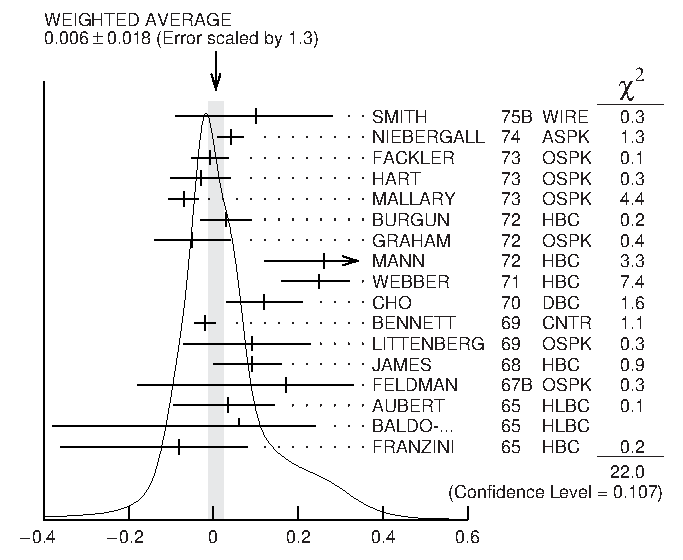
\includegraphics{filename.pdf}
	\caption{Example default figure}
	\label{examples:fig:example}
\end{pdgxfigure}
\end{verbtex}
\begin{pdgxfigure}[place=t]
	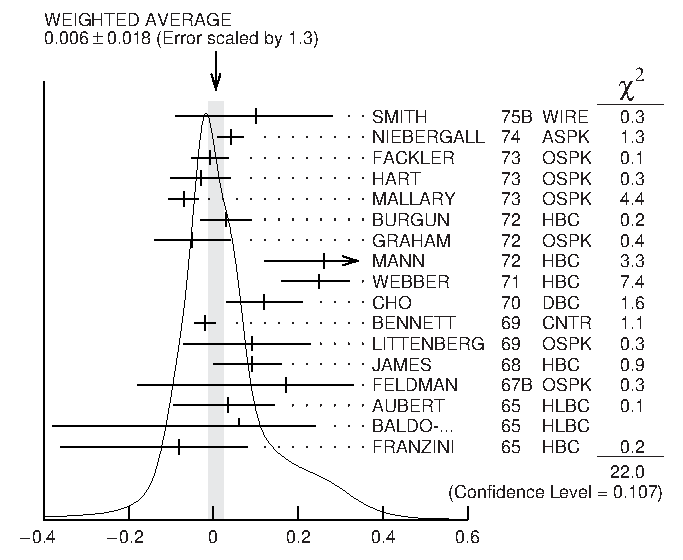
\includegraphics{filename.pdf}
	\caption{Example default figure}
	\label{examples:fig:example}
\end{pdgxfigure}

A double wide figure, shown in Fig.~\ref{examples:fig:example2}:
\begin{verbtex}
\begin{pdgxfigure}[wide=true,place=h, webwidth=0.45\linewidth, 
		bookwidth=0.9\linewidth] 
	%width key applies to all includegraphics instances
	%compiling in different versions will produce different widths
	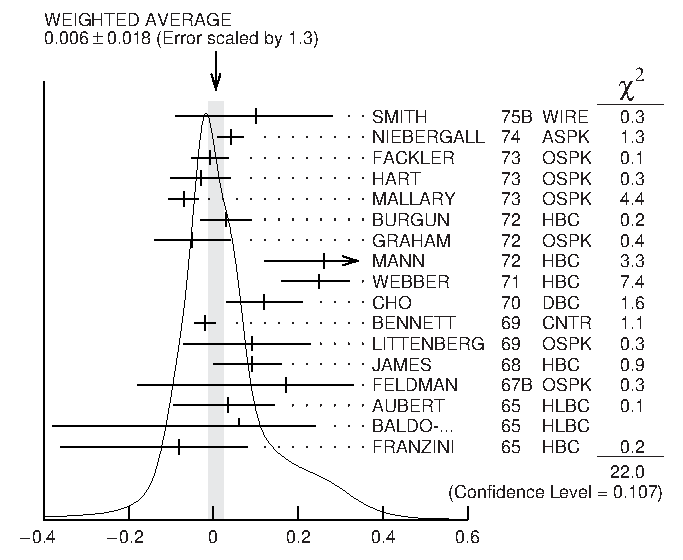
\includegraphics{filename.pdf}\hfill
	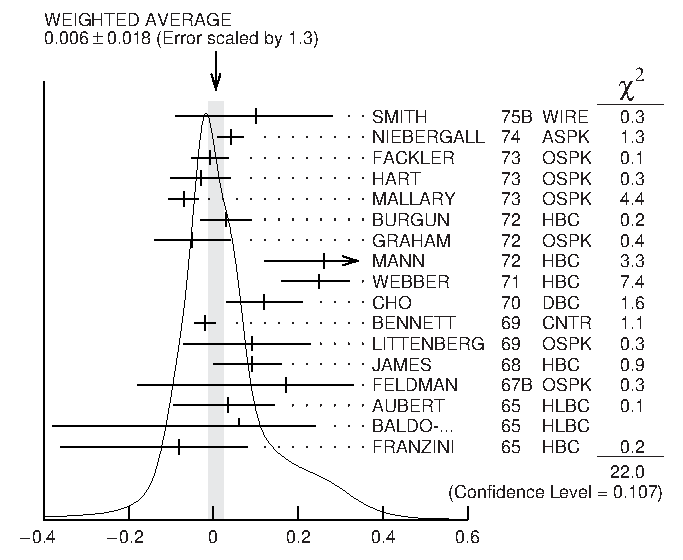
\includegraphics{filename.pdf}
	\caption{Example double wide figure, 
		with different book and web versions}
	\label{examples:fig:example2}
\end{pdgxfigure}
\end{verbtex}
\begin{pdgxfigure}[wide=true,place=h,width=0.45\textwidth] 
	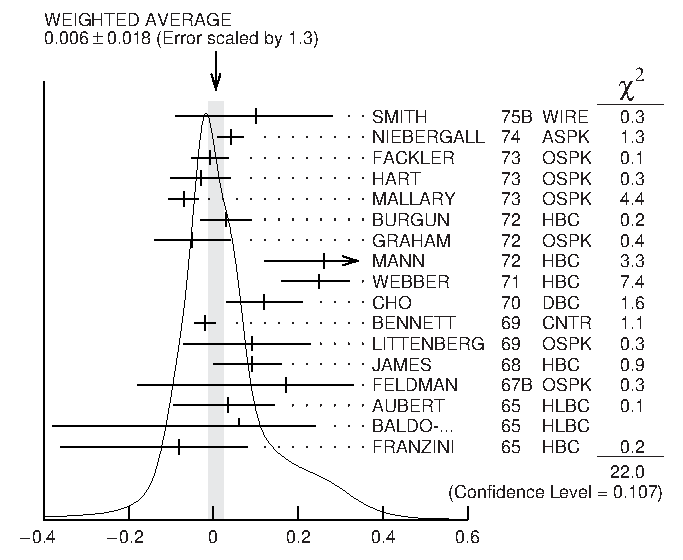
\includegraphics{filename.pdf}\hfill
	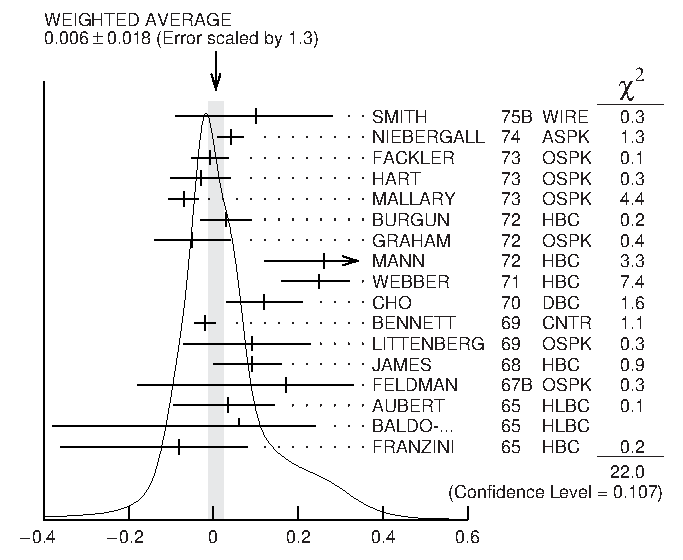
\includegraphics{filename.pdf}
	\caption{Example double wide figure, with different book and web versions}
	\label{examples:fig:example2}
\end{pdgxfigure}

A double wide figure with separate option and scaling keys, shown in Fig.~\ref{examples:fig:example3}:
\begin{verbtex}
\begin{pdgxfigure}[wide=true,place=h,width = 0.3\linewidth] 
	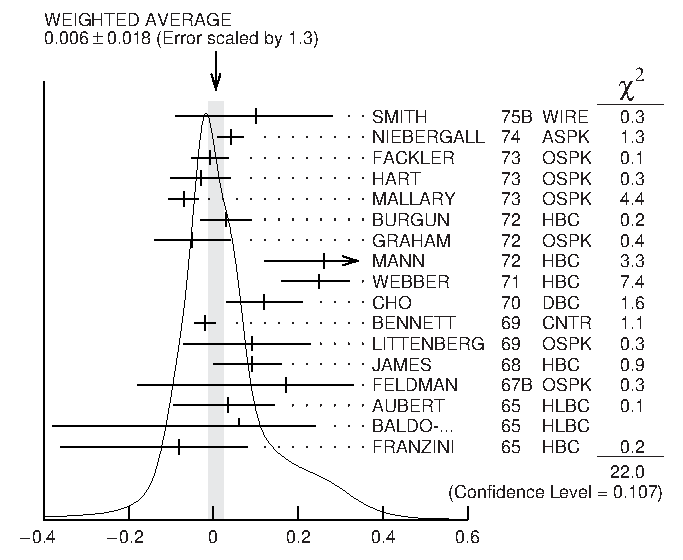
\includegraphics{filename.pdf}\hspace{1cm}
	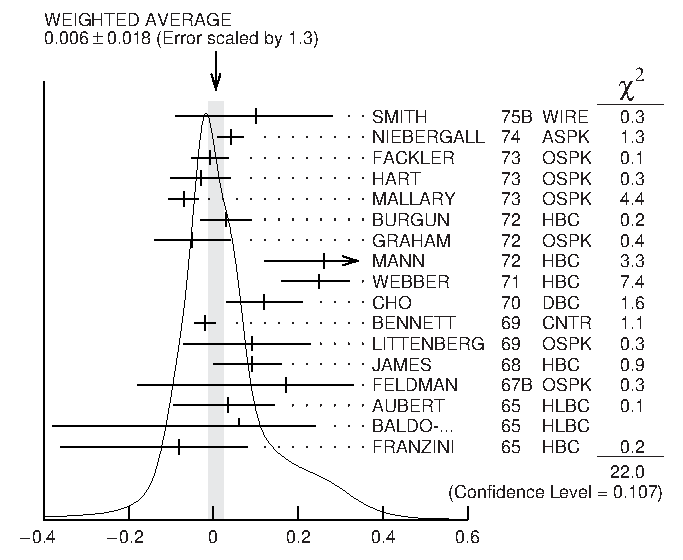
\includegraphics[width = !,scale =0.3,angle = 90]{filename}
	\caption{Example double figure, 
		with separate option and scaling keys, in both book and web versions}
	\label{examples:fig:example3}
\end{pdgxfigure}
\end{verbtex}
\begin{pdgxfigure}[wide=true,place=h,width = 0.3\linewidth] 
	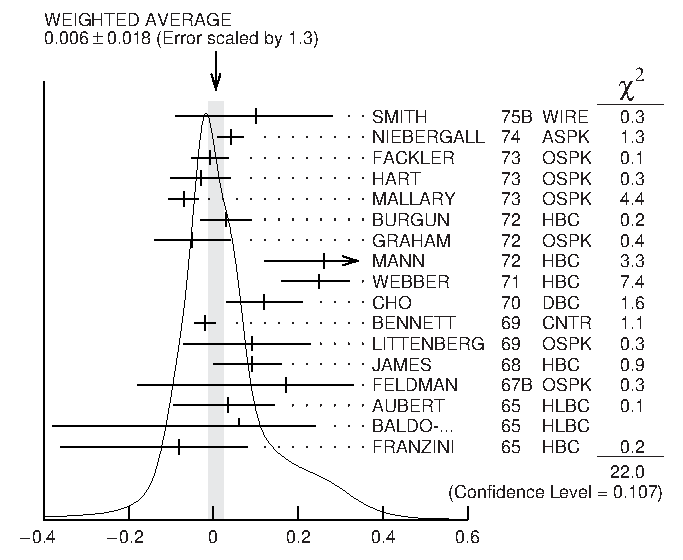
\includegraphics{filename.pdf}\hspace{1cm}
	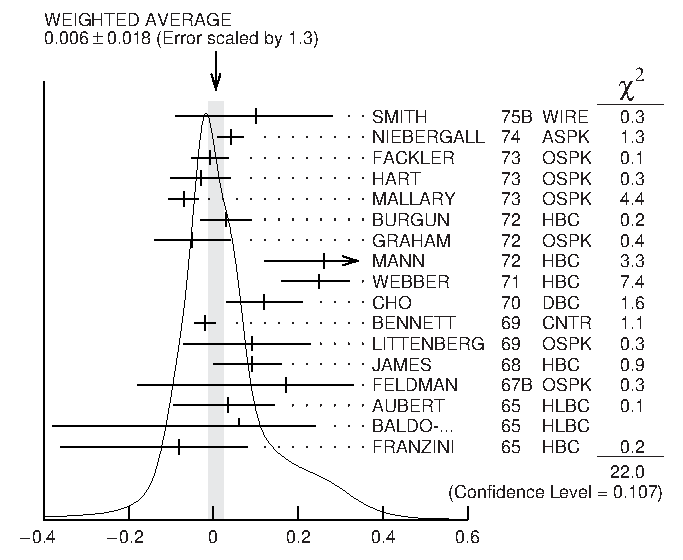
\includegraphics[width = !,scale =0.3,angle = 90]{filename}
	\caption{Example double wide figure, with separate option and scaling keys, in both book and web versions}
	\label{examples:fig:example3}
\end{pdgxfigure}

\Isubsection{\invt{pdgfigure} commands}
To add a figure, one may also use the \lstinline{\pdgfigure} or \lstinline{\pdgwidefigure} commands 
to typeset a single-column figure or double-column wide figure (for the book version), respectively. 
To include two images in one figure one may use \lstinline{\pdgdoublefigure}.
These commands are less powerful than \invt{pdgxfigure}, but automatically incorporate all PDG styles.

The macros \lstinline{\pdgfigure} and \lstinline{\pdgwidefigure} take the following arguments:
\begin{verbtex}
	\pdgfigure{<filename>}
	{<caption>}{<label>}{<placement options>}
	{<other option keys>}
\end{verbtex}
\vspace{-10pt}
while the macro \lstinline{\pdgdoublefigure} takes the following arguments:
\begin{verbtex}
	\pdgdoublefigure{<filename1>}{<filename2>}
	{<caption>}{<label>}{<placement options>}
	{<other option keys>}
\end{verbtex}
Some examples of the \invt{pdgfigure} commands are shown in Figs.~\ref{examples:fig:ideogram1}, \ref{examples:fig:ideogram2} and \ref{examples:fig:ideogram3}, respectively:
\begin{verbtex}
	\pdgfigure{filename.pdf}{Figure with caption and label}
	{examples:fig:ideogram1}{ht!}{}
	
	\pdgdoublefigure{filename.pdf}{filename.pdf}
	{Two figures, with caption and label, reduced in size}
	{examples:fig:ideogram2}{ht!}{width=0.3\textwidth}
	
	\pdgwidefigure{filename.pdf}{Wide figure}
	{examples:fig:ideogram3}{t}{}
\end{verbtex}
\FloatBarrier
\pdgfigure{filename.pdf}{Figure with caption and label}{examples:fig:ideogram1}{ht!}{}
\pdgdoublefigure{filename.pdf}{filename.pdf}{Two figures, with caption and label, reduced in size}{examples:fig:ideogram2}{ht!}{width=0.3\textwidth}
\pdgwidefigure{filename.pdf}{Wide figure}{examples:fig:ideogram3}{t}{}
\FloatBarrier

\Isection{Tables}
\label{sec:tables}
\Isubsection{ \invt{pdgxtable} and \invt{pdgxtabular}}
The PDG class provides multipurpose table and tabular environments, \invt{pdgxtable} and \invt{pdgxtabular}. 
These operate similarly to the standard \invt{table} and \invt{tabular} environments: \invt{(pdgx)table} creates a floating environment, 
while \invt{(pdgx)tabular} creates the actual tabulated display. 

The \lstinline!\caption! and \lstinline!\label! commands may be used as in the usual \invt{table} environment.
\textbf{Note: A table caption should be placed above the table.}
In addition, \invt{pdgxtable} takes a wide array of additional option keys that implement features and formatting of the prior PDG table commands/environments.  
These include keys that control placement, multicolumn spanning, version-specific widths and scaling (see Sec.~\ref{sec:ginkeys}), rotation, stretching, and caption widths.
The generic usage is
\begin{verbtex}
\begin{pdgxtable}[<option keys>]
	\caption{This is a PDG table}
	\label{tab:label}
	\begin{pdgxtabular}{<column settings>} % the usual c, l, r, | etc
		\pdgtableheader{...} %column header & separated entries go here
		%table & separated entries go here
	\end{pdgxtabular}
	%multiple pdgtabular environments are allowed
\end{pdgxtable}
\end{verbtex}

As for the usual \invt{table} environment, one may include multiple \invt{pdgxtabular}s in a single \invt{pdgxtable}.
While the \invt{pdgxtable} environment has default handling for caption widths in wide and regular tables, for both book and web versions, 
absolute control of the caption width can be implmented with a \lstinline{\captionsetup} command inside the \invt{pdgxtable} environment. 
For example \lstinline!\captionsetup{width=\linewidth}! gives a full width caption.

\Isubsection{Available keys for \invt{pdgxtable}}
Following is a list of available optional keys, and default settings if not invoked.
As usual, keys are evaluated left to right. 
While, the version-general \invt{width} key can be used (and will override any preceeding version-specfic width key), 
there is no version-general \invt{scale} key. 
Scaling of the tables is best done with the \invt{<version>scale} keys.

\begin{itemize}
	\item \invt{place}: Takes any combination of \invt{h}, \invt{t}, \invt{b}, \invt{p} (with optional \invt{\!}) that specifies float placement. Default is \invt{\!ht}.
	\item \invt{wide}: Takes \invt{true} or \invt{false} to specify the table as full page width in either single or two column mode. Default is \invt{false}.
	\item \invt{width} or \invt{<version>width}: Sets the version specific maximum width of the table bounding box. 
	Default is the maximum text width implied by the \invt{wide} key setting.
	Width settings exceeding this default are ineffective. Footnotes are scaled, but caption width is not affected.
	\item \invt{<version>scale}: Scales the table according to float value passed to the key. 
	For overwide tables, there is always a value $<1$ at which the table will be properly set to maximum page width.
	Footnotes are scaled, but caption width is not affected. Note the global \invt{scale} is disabled for \invt{pdgxtable}.
	\item \invt{<version>bbscale}: Scales the bounding box of the table. 
	For some overwide tables that are larger than the nominal page width, simply rescaling down the table does not allow the table to be properly aligned on the page.
	This key can be increased above $1$ (the default), to provide a sufficiently large bounding box for the table, that may then be scaled down to size with correct alignment.
	\item \invt{widecaptionscale}: For \invt{wide = true} tables, scales the caption width with respect to the maximum page width. Default is $0.75$.
	\item \invt{narrowcaptionscale}: For \invt{wide = false} or default tables, scales the caption width with respect to the maximum column width. Default is $0.9$.
	\item \invt{rotated}: Takes \invt{left} or \invt{right} to rotate the table, but not the caption, $90^\circ$ anticlockwise or clockwise, respectively. 
	The caption may be rotated independently, as needed with a \lstinline{\rotatebox}.
	\item \invt{sideways}: Takes \invt{true} or \invt{false} to rotate the table, including the caption, $90^\circ$ anticlockwise or clockwise, 
	according to whether the page number is even or odd.
	In a sideways table, other key width and scaling settings are still effective, but scale with respect to the page height. 
\end{itemize}


\Isubsection{Examples}
Some (simple) examples of \invt{pdgxtable} can be found in Table~\ref{examples:tab:styles} and Sec~\ref{sec:macros}.
For example, Tab.~\ref{examples:tab:styles} is typeset as
\begin{verbtex}
\begin{pdgxtable}[place=h,bookscale = 0.9,bookbbscale=2]
	\caption{Styles for the different typesetting versions}
	\label{examples:tab:styles}
	\begin{pdgxtabular}{ccccc}
		Version 		& Columns  & Font size 	& Helper Tags\footnote{
			Tags for each equation, table, figure, and bibliography entry 
			are displayed in margin or interspaced} & Line numbers\\
		\hline
		draft	& 1		   & 11pt		& Yes & Yes \\
		...
	\end{pdgxtabular}
\end{pdgxtable}
\end{verbtex}

Tables~\ref{examples:tab:commu} and~\ref{examples:tab:commp} are typeset as a two \invt{pdgxtabular}s in a single \invt{pdgxtable}, via
\begin{verbtex}
\begin{pdgxtable}[wide=true, place=!ht, webscale = 0.8]
	\caption{Common units}
	\label{examples:tab:commu}
	\begin{pdgxtabular}{lr | lr | lr}
		\showsymbol{\TeV} &  \showsymbol{\syin} & \showsymbol{\barn}   \\
		...
	\end{pdgxtabular}
	\caption{Common particles}
	\label{examples:tab:commp}
	\begin{pdgxtabular}{lr | lr | lr}
   		\showsymbol{\pp} &  \showsymbol{\ee} & \showsymbol{\pizero}   \\
  		...
	\end{pdgxtabular}
\end{pdgxtable}
\end{verbtex}

\Isubsection{Common problems and recommendations}
The \invt{pdgxtabular} environment is capable of handling the usual \lstinline{\multicolumn} and \lstinline{\multirow} objects, 
that allow for more complicated tables with cells spanning multiple rows and/or columns. 
We recommend avoiding use of \lstinline{\multispan}. 
For multiline cells, the \lstinline{\makecell} command from the \invt{makecell} package is recommended.

\Isection{Labels and referencing}
\label{sec:labels}

\Isubsection{Style guide}
As usual, the \lstinline{\label} and \lstinline{\ref} commands (and their derivatives) may be used to reference equations, tables, figures, and so on. 
To permit easy cross-referencing throughout the entire review, we request that you use the following labelling convention: \invt{BASENAME:type:name}
with \invt{type} corresponding to one of the following options
\begin{itemize}
\item {\tt fig} for figures
\item {\tt eq } for equation
\item {\tt tab} for tables
\item {\tt sec} for section, subsection etc..
\item {\tt foot} for footnotes.
\end{itemize}

\Isubsection{Missing references}

In default LaTeX, missing references are typically typeset as ``\textbf{??}''. 
To improve the typesetting experience, the \lstinline{\ref} command has been modified in the PDG class so that missing reference keys are printed out explicitly: 
For instance, a \lstinline!\ref{eqn:name}! that references a missing label called \invt{eqn:name}, will display as \ref{eqn:name}.
Similarly, the \lstinline{\cite} command will explicitly print out missing citation references. E.g. 
a \lstinline!\cite{name:2021ab}! that references a missing label called \invt{name:2021ab}, will display as \cite{name:2021ab}

\Isubsection{Cross-review referencing}
It is occasionally necessary or useful to reference (sub)sections, equations, figures, tables and so on belonging to other reviews or other reviews themselves. 
\textbf{Note:} Please use the \lstinline{\crossref} command for cross-review referencing.

Implementing a cross-reference to another review requires knowledge of its  \invt{BASENAME}:  
You must use the \invt{BASENAME} associated with the target review, not the \invt{BASENAME} of the review you're currently working on. 
To identify the  \invt{BASENAME} of another review, login into the \href{https://pdgworkspace.lbl.gov/Reviews.action}{PDG Workspace} (click to be redirected). 
Under \emph{Reviews} select from the drop-down menu \emph{All reviews}. 
Click on the title of the review you are interested in, and then select the \emph{Technical details} tab. 
The \invt{BASENAME} is the first entry.


If the full \invt{BASENAME:type:name} reference is known, you may include it with the usage \\
\lstinline!\crossref{BASENAME:type:name}!. 
This will typeset in your document as ``\crossref{BASENAME:type:name}'', because your local auxiliary files do not have the reference information of the other review.
PDG editorial staff will implement the cross-reference properly, when your review is prepared for production.

If the \invt{BASENAME:type:name} reference is not known, or the authors of the other review did not label the obect that you wish to reference, 
you may instead provide any descriptive argument to \lstinline{\crossref}. 
For example, \lstinline!\crossref{Equation 34.1.10}!.  
PDG editorial staff will implement the cross-reference properly, when your review and the other review are prepared for production.

\Isubsection{Booklet labeling and referencing}
If your review has a booklet version, it needs to be prepared at the same time as you prepare your full review.
The content to be displayed in the booklet needs to be included in \invt{BASENAME-booklet.tex}. 

The numerical tags for equations, tables, and figures in the booklet version of a review should match the tags in the full version. 
This can be achieved automatically in the booklet version by using a \lstinline!\tag{\ref{BASENAME:type:name}}! construction instead of \lstinline{\label}
to refer to the reference in the full version.
For example, if the full version has a labelled equation
\begin{verbtex}
\begin{equation}
	\label{BASENAME:eq:name}
	...
\end{equation}
\end{verbtex}
then including in \invt{BASENAME-booklet.tex}
\begin{verbtex}
\begin{equation}
	\tag{\ref{BASENAME:eq:name}}
	...
\end{equation}
\end{verbtex}
will automatically label the equation correctly. 
To achieve the same result for figures and tables, one may place in the booklet version
\begin{verbtex}
	\renewcommand{\thetable}{\ref{BASENAME:type:name}}
	\renewcommand{\thefigure}{\ref{BASENAME:type:name}}
\end{verbtex}
before each table or figure environment, respectively. 


\Isection{Index entries}
\label{sec:index}

Review authors should think about any keywords that should be included into the index of the Review of Particle Physics. PDG uses the standard \LaTeX\  \invt{makeidx} package. Thus an entry ``sample text'' can be added to the index by placing
\begin{verbtex}
\index{sample text}
\end{verbtex}
at the appropriate place in the source file. Formatting of entries with Greek letters or math symbols as well as subentries are also supported. For example
\begin{verbtex}
\index{sigma@$\$$\sigma$\$$} 
\end{verbtex}
creates an index entry $\sigma$ in the proper alphabetical order, while
\begin{verbtex}
\index{Searches!Axion searches} 
\end{verbtex}
produces a subentry ``Axion searches'' under the ``Searches'' index entry.

All index entries defined in a given review will be shown on the last page when the draft version is made. PDG staff will standardize all index entries during the final processing of all reviews. Therefore what matters is not the final formatting of index entries but that all relevant entries are added in the correct place.


\Isection{Bibliography}
\label{sec:cites}

Citations are handled using BibTeX. To add a citation to your review:
\begin{itemize}
\item Look up the reference in INSPIRE and download its BibTeX entry (see bottom of the \emph{Information} tab for the article, under \emph{Export}).
\item Add the BibTeX entry to the \invt{BASENAME.bib} file. Note the article tag assigned by INSPIRE: You can see it in the first line of the BibTeX entry, after \lstinline!@article{!.
\item Cite the reference with \lstinline{\cite}, using the article tag assigned by INSPIRE.
\end{itemize}

For example, to add a reference to the Review of Particle Physics (2018) 
add the following code to \invt{BASENAME.bib}:
\begin{verbtex}
@article{Tanabashi:2018oca,
      author         = "Tanabashi, M. and others",
      title          = "{Review of Particle Physics}",
      collaboration  = "Particle Data Group",
      journal        = "Phys. Rev.",
      volume         = "D98",
      year           = "2018",
      number         = "3",
      pages          = "030001",
      doi            = "10.1103/PhysRevD.98.030001",
      SLACcitation   = "%%CITATION = PHRVA,D98,030001;%%"
 }
\end{verbtex}
and then one may add a reference to it in \invt{BASENAME-main.tex} via \lstinline!\cite{Tanabashi:2018oca}!.

If a BibTeX entry downloaded from INSPIRE does not render correctly, 
you should first make sure you have the latest PDG style files, by running \invt{svn update} (after committing any edits you have made).
If this doesn't fix the issue please contact \invt{latexsupport@pdg.lbl.gov} for advice.  
If it appears, however, to be simply a mistake in INSPIRE's entry, 
rename the label to the form \invt{BASENAME:<INSPIRE label>} and then edit the entry as needed.
\textbf{Please do not edit entries downloaded from INSPIRE without changing the label.}
Changing the label will permit PDG editorial staff to easily identify and track edited citations, as well as notify INSPIRE of required corrections.
In case the reference does not appear in INSPIRE at all, please also use the convention for the label: \invt{BASENAME:name}.

Multiple references can be added to a single set of brackets with \lstinline!\cite{cite-key-1,cite-key-2,...}!.
One may group multiple references into the same numerical citation tag, using a \invt{*} prefix on subsequent citation keys: For example \lstinline!\cite{cite-key-1,*cite-key-2,*cite-key-3}!.
If a paper citation key is preceded by the asterisk, it can't be cited separately later, and doing so will result in a compilation error.
We recommend citing papers individually, without using the asterisk to group them.


\Isection{Footnotes}
Footnote styles are standardized throughout the review. In (rare) cases that the style needs to be changed, this is achieved via \lstinline!\setfootnotestyle{<style>}!,
where \invt{<style>} can be \lstinline{\fnsymbol} or \lstinline{\alph}, \lstinline{\Alph}, \lstinline{\arabic}, \lstinline{\roman}, \lstinline{\Roman} etc.

Sometimes the \LaTeX \ engine miscalculates the amount of space required for a footnote, resulting in overprinting of the footer.
One can help the engine obtain a better estimate by adjusting the effective page size. 
This can be done by placing \lstinline!\enlargethispage{-2\baselineskip}! somewhere just before the \lstinline{\footnote}; the \invt{-2} may be changed to any number. 

\Isection{Miscellaneous control commands}

\Isubsection{Unbalanced last page}
In the book version, the columns of the final page are automatically balanced. 
If this behavior is undesired, it may be altered by invoking \lstinline!\balancedlastpagefalse!.
The invocation may be added anywhere in the document.

\Isubsection{Blank last page}
In the book version, a blank final page may be added via \lstinline!\blankendpagetrue!.
The invocation may be added anywhere in the document.

\Isubsection{Book-only reviews}
Certain reviews are typeset for the web using the book version formatting. 
This is enforced automatically within the PDG system by \lstinline!\def\iswebbook{1}! before the \lstinline{\documentclass} invocation. 
The draft version, however, for such reviews are typeset in the usual draft/web format.

\clearpage
\Isection{PDG Macros}
\label{sec:macros}

\begin{pdgxtable}[wide=true, place=!ht, webscale = 0.8]
	\vspace{-10pt}
	\caption{Common units}
	\label{examples:tab:commu}
	\begin{pdgxtabular}{lr | lr | lr}
		\showsymbol{\TeV     } &  \showsymbol{\syin} & \showsymbol{\barn     }   \\
		\showsymbol{\MeV     } &  \showsymbol{\inch} & \showsymbol{\mbarn    }   \\
		\showsymbol{\keV     } &  \showsymbol{\ft  } & \showsymbol{\microbarn}   \\
		\showsymbol{\eV      } &  \showsymbol{\km  } & \showsymbol{\nb       }   \\
		\showsymbol{\GeVc    } &  \showsymbol{\m   } & \showsymbol{\pb       }   \\
		\showsymbol{\GeVcSq  } &  \showsymbol{\cm  } & \showsymbol{\fb       }   \\
		\showsymbol{\GeVcc   } &  \showsymbol{\mm  } & \showsymbol{\invnb    }   \\
		\showsymbol{\GeVccSq } &  \showsymbol{\mum } & \showsymbol{\invpb    }   \\
		\showsymbol{\MeVc    } &  \showsymbol{\nm  } & \showsymbol{\invfb    }   \\
		\showsymbol{\MeVcc   } &  \showsymbol{\fm  } & \showsymbol{\invab    }   \\
		\showsymbol{\invps   } &  \showsymbol{\nm  } & \showsymbol{\lum      }   \\
			&&  \showsymbol{\ma  } &&  \\
		\showsymbol{\degr    }  &  \showsymbol{\cma } && \\
			&&  \showsymbol{\mma } &&   \\
			&&  \showsymbol{\muma} &&   \\
	\end{pdgxtabular}
	\vspace{10pt}
	\caption{Common particles}
	\label{examples:tab:commp}
	\vspace{-10pt}
	\begin{pdgxtabular}{lr | lr | lr}
   \showsymbol{\pp         } &  \showsymbol{\ee           } & \showsymbol{\pizero   }   \\
   \showsymbol{\pbar       } &  \showsymbol{\epm          } & \showsymbol{\piplus   }   \\
   \showsymbol{\ppbar      } &  \showsymbol{\epem         } & \showsymbol{\piminus  }   \\
   \showsymbol{\tbar       } &  \showsymbol{\en           } & \showsymbol{\pipm     }   \\
   \showsymbol{\ttbar      } &  \showsymbol{\ep           } & \showsymbol{\pimp     }   \\
   \showsymbol{\bbar       } &  \showsymbol{\mumu         } & \showsymbol{\etaprime }   \\
   \showsymbol{\bbbar      } &  \showsymbol{\mun          } & \showsymbol{\Kzero    }   \\
   \showsymbol{\cbar       } &  \showsymbol{\mup          } & \showsymbol{\Kzerobar }   \\
   \showsymbol{\ccbar      } &  \showsymbol{\tautau       } & \showsymbol{\kaon     }   \\
   \showsymbol{\sbar       } &  \showsymbol{\taup         } & \showsymbol{\Kplus    }   \\
   \showsymbol{\ssbar      } &  \showsymbol{\taum         } & \showsymbol{\Kminus   }   \\
   \showsymbol{\ubar       } &  \showsymbol{\lepton       } & \showsymbol{\KzeroL   }   \\
   \showsymbol{\uubar      } &  \showsymbol{\leptonm      } & \showsymbol{\Kzerol   }   \\
   \showsymbol{\dbar       } &  \showsymbol{\ellm         } & \showsymbol{\Klong    }   \\
   \showsymbol{\ddbar      } &  \showsymbol{\leptonp      } & \showsymbol{\KzeroS   }   \\
   \showsymbol{\fbar       } &  \showsymbol{\ellp         } & \showsymbol{\Kzeros   }   \\
   \showsymbol{\ffbar      } &  \showsymbol{\leptonlepton } & \showsymbol{\Kshort   }   \\
   \showsymbol{\qbar       } &  \showsymbol{\ellell       } & \showsymbol{\Kstar    }   \\
   \showsymbol{\qqbar      } &  \showsymbol{\enu          } & \showsymbol{\jpsi     }   \\
   \showsymbol{\nbar       } &  \showsymbol{\munu         } & \showsymbol{\Jpsi     }   \\
   \showsymbol{\nnbar      } &  \showsymbol{\taunu        } & \showsymbol{\psip     }   \\
   \showsymbol{\neutron    } &  \showsymbol{\lnu          } & \showsymbol{\chic     }   \\
   \showsymbol{\antineutron} &  \showsymbol{\nub          } & \showsymbol{\UoneS    }   \\
   \showsymbol{\deuteron   } &  \showsymbol{\nunub        } & \showsymbol{\chib     }   \\
   \showsymbol{\Zzero      } &  \showsymbol{\nue          } & \showsymbol{\Dstar    }   \\
   \showsymbol{\Zboson     } &  \showsymbol{\nueb         } & \showsymbol{\Bd       }   \\
   \showsymbol{\Wplus      } &  \showsymbol{\nuenueb      } & \showsymbol{\Bs       }   \\
   \showsymbol{\Wminus	   } &  \showsymbol{\num          } & \showsymbol{\Bu       }   \\
   \showsymbol{\Wboson	   } &  \showsymbol{\numb         } & \showsymbol{\Bc       }   \\ 
   \showsymbol{\Wpm   	   } &  \showsymbol{\numnumb      } & \showsymbol{\Lb       }   \\
   \showsymbol{\Wmp        } &  \showsymbol{\nut          } & \showsymbol{\Bstar    }   \\
   \showsymbol{\Hzero } &  \showsymbol{\nutb         } & \showsymbol{\BoBo     }   \\
   \showsymbol{\Hboson}  &	\showsymbol{\nutnutb      } & \showsymbol{\BodBod   }    \\		    
   \showsymbol{            } &	\showsymbol{              } & \showsymbol{\BosBos   }    \\		    
   \showsymbol{            } &	\showsymbol{              } & \showsymbol{\LambdaStar}  \\
	\end{pdgxtabular}
\end{pdgxtable}

\begin{pdgxtable}[wide=true, place=h, webscale = 0.8]
	\caption{Hypothetical particles}
	\begin{pdgxtabular}{lr | lr | lr}
   \showsymbol{\Azero }      &  \showsymbol{\gravino   } & \showsymbol{\slepton   }   \\
   \showsymbol{\hzero }      &  \showsymbol{\Zprime    } & \showsymbol{\sleptonL  }   \\
   \showsymbol{\Hzero }      &  \showsymbol{\Zstar     } & \showsymbol{\sleptonR  }   \\
   \showsymbol{\Hplus }  	  &  \showsymbol{\squark    } & \showsymbol{\sel       }   \\
   \showsymbol{\Hminus}       &  \showsymbol{\squarkL   } & \showsymbol{\selL      }   \\
   \showsymbol{\Hpm   }   	&  \showsymbol{\squarkR   } & \showsymbol{\selR      }   \\
   \showsymbol{\Hmp   }       &  \showsymbol{\gluino    } & \showsymbol{\smu       }   \\
   \showsymbol{\ggino }     &  \showsymbol{\stop      } & \showsymbol{\smuL      }   \\
   \showsymbol{\chinop}      &  \showsymbol{\stopone   } & \showsymbol{\smuR      }   \\
   \showsymbol{\chinom}      &  \showsymbol{\stoptwo   } & \showsymbol{\stau      }   \\
   \showsymbol{\chinopm}      &  \showsymbol{\stopL     } & \showsymbol{\stauL     }   \\
   \showsymbol{\chinomp}     &  \showsymbol{\stopR     } & \showsymbol{\stauR     }   \\
   \showsymbol{\chinoonep}     &  \showsymbol{\sbottom   } & \showsymbol{\stauone   }   \\
   \showsymbol{\chinoonem}   &  \showsymbol{\sbottomone} & \showsymbol{\stautwo   }   \\
   \showsymbol{\chinoonepm}   &  \showsymbol{\sbottomtwo} & \showsymbol{\snu       }   \\
   \showsymbol{\chinotwop}  &  \showsymbol{\sbottomL  } & \showsymbol{           }   \\
   \showsymbol{\chinotwom}   &  \showsymbol{\sbottomR  } & \showsymbol{           }   \\
   \showsymbol{\chinotwopm}   &  \showsymbol{           } & \showsymbol{           }   \\
   \showsymbol{\nino}  &  \showsymbol{           } & \showsymbol{           }   \\
   \showsymbol{\ninoone}        &  \showsymbol{           } & \showsymbol{           }   \\
   \showsymbol{\ninotwo}     &  \showsymbol{           } & \showsymbol{           }   \\
   \showsymbol{\ninothree}     &  \showsymbol{           } & \showsymbol{           }   \\
   \showsymbol{\ninofour}   &  \showsymbol{           } & \showsymbol{           }   \\
	\end{pdgxtabular}
\vspace*{10pt}
	\caption{Useful symbols for proton-proton physics}
\vspace*{-10pt}	
	\begin{pdgxtabular}{lr | lr }
   \showsymbol{\pT  }      &  \showsymbol{\rts }   \\
   \showsymbol{\pt  }      &  \showsymbol{\sqs } \\
   \showsymbol{\ET  }      &  \showsymbol{\mh}  \\
   \showsymbol{\eT  }      &  \showsymbol{\mW}  \\
   \showsymbol{\et  }      & \showsymbol{\mZ}   \\
   \showsymbol{\HT  }      & \showsymbol{\mH}   \\
   \showsymbol{\pTsq}      &&   \\
   \showsymbol{\MET }      &&   \\
   \showsymbol{\met }      &&   \\
   \showsymbol{\Ecm }      &&   \\
	\end{pdgxtabular}
\vspace*{10pt}
	\caption{Monte Carlo Generators}
\vspace*{-10pt}		
	\begin{pdgxtabular}{lr | lr | lr}	
   \showsymbol{\ACERMC    }      &  \showsymbol{\MCatNLO   } & \showsymbol{\Comphep    }   \\
   \showsymbol{\ALPGEN    }      &  \showsymbol{\AMCatNLO  } & \showsymbol{\Prospino   }   \\
   \showsymbol{\GEANT     }      &  \showsymbol{\MCFM      } & \showsymbol{\LO         }   \\
   \showsymbol{\Herwigpp  }      &  \showsymbol{\METOP     } & \showsymbol{\NLO        }   \\
   \showsymbol{\HERWIGpp  }      &  \showsymbol{\POWHEG    } & \showsymbol{\NLL        }   \\
   \showsymbol{\Herwig    }      &  \showsymbol{\POWHEGBOX } & \showsymbol{\NNLO       }   \\
   \showsymbol{\HERWIG    }      &  \showsymbol{\POWPYTHIA } & \showsymbol{\muF        }   \\
   \showsymbol{\JIMMY     }      &  \showsymbol{\PROTOS    } & \showsymbol{\muR        }   \\
   \showsymbol{\MADSPIN   }      &  \showsymbol{\PYTHIA    } & \showsymbol{            }   \\
   \showsymbol{\MADGRAPH  }      &  \showsymbol{\SHERPA    } & \showsymbol{            }   \\
   \showsymbol{\MGMCatNLO }      &  \showsymbol{           } & \showsymbol{            }   \\
	\end{pdgxtabular}
\end{pdgxtable}

\Isection{Tables: Legacy commands}

Though no longer recommended, legacy \lstinline{\pdgtable} or \lstinline{\pdgwidetable} commands 
to typeset a single-column table or double-column wide table (for the book version), respectively.
The \lstinline{\pdgtableheader} macro may be used in the first line of the table to automatically typeset a header.

The macros \lstinline{\pdgtable} and \lstinline{\pdgwidetable} take the following arguments:
\begin{verbtex}
	\pdgtable{<column styles>}
	{<caption>}{<label>}{<option keys>}
\end{verbtex}
Some examples usages of these commands follow, in Tables~\ref{examples:tab:table1}, \ref{examples:tab:table2} and~\ref{examples:tab:table3} below.
\begin{verbtex}
\begin{pdgtable}{c c c} 
	{Table}{examples:tab:table1}{h!}
	\pdgtableheader{ Column 1 & Column 2 & Column 3}
	row1  & 1  & 2\\
	row2  & 1  & 2\\
	row3  & 1  & 2\\
\end{pdgtable}
\end{verbtex}   
\begin{verbtex}
\begin{pdgtable}{|c | c | c | c|} 
	{Multicolumn table}{examples:tab:table2}{h!}
	\pdgtableheader{ \multicolumn{2}{c}{Column 1} & 
	\multicolumn{2}{c}{Column 2}}
	\pdgtableheader{ A & B& C & D }
	row1  & 1 & 2 &3 \\
	row2  & 1 & 2 &3 \\
\end{pdgtable}
\end{verbtex}  
\begin{verbtex}
\begin{pdgtable}{c l}
	{Table with footnotes}{examples:tab:table3}{}
	One value & another\footnote{This is something to notice
	\label{kmmix:foot:one}}\\
	Two values\footref{kmmix:foot:one} & another \\
\end{pdgtable}
\end{verbtex} 
 
\FloatBarrier 
\begin{pdgtable}{c c c} 
{Table}{examples:tab:table1}{h!}
\pdgtableheader{ Column 1 & Column 2 & Column 3}
row1  & 1  & 2\\
row2  & 1  & 2\\
row3  & 1  & 2\\
\end{pdgtable}
\begin{pdgtable}{|c | c | c | c|} 
{Multicolumn table}{examples:tab:table2}{h!}
\pdgtableheader{ \multicolumn{2}{|c|}{Column 1} & 
\multicolumn{2}{|c|}{Column 2}}
\pdgtableheader{ A & B& C & D }
row1  & 1 & 2 &3 \\
row2  & 1 & 2 &3 \\
\end{pdgtable}
\begin{pdgtable}{c l}
{Table with footnotes}{examples:tab:table3}{}
One value & another\footnote{This is something to notice\label{kmmix:foot:one}}\\
Two values\footref{kmmix:foot:one} & another \\
\end{pdgtable}



% References
% ----------
% The following line includes your bibliography using BibTeX. In case you do not
% yet use BibTex, you can put your bibliography below (using a series of \bibitem entries).
% Please  note that using BibTeX will become mandatory in the future.
%\IfFileExists{ml.bib, review.bib, biblio.bib}{\putbib[ml,review,biblio]}{}
\IfFileExists{ml.bib}{\putbib[ml,review,biblio,sbi]}{}



